\documentclass[10pt,a4paper]{report}
\usepackage[T1]{fontenc}
\usepackage[utf8]{inputenc}
\usepackage[margin=2.2cm,headheight=14pt]{geometry}
\usepackage{helvet}\renewcommand{\familydefault}{\sfdefault}
\usepackage{booktabs,longtable,array,xcolor,colortbl,enumitem,titlesec,graphicx,caption,float}
\usepackage{fancyhdr,lastpage,tocloft}
\usepackage[hidelinks]{hyperref}
\definecolor{navy}{HTML}{1F3A68}\definecolor{band}{HTML}{EEF2F7}
\titleformat{\chapter}[hang]{\LARGE\bfseries\color{navy}}{\thechapter}{12pt}{}
\titlespacing*{\chapter}{0pt}{-20pt}{14pt}
\titleformat{\section}{\large\bfseries\color{navy}}{\thesection}{8pt}{}
\titleformat{\subsection}{\normalsize\bfseries\color{navy}}{\thesubsection}{8pt}{}
\setlist{nosep,leftmargin=1.3em,topsep=2pt}
\setlength{\parindent}{0pt}\setlength{\parskip}{5pt}
\captionsetup{font=small,labelfont={bf,color=navy},justification=raggedright,singlelinecheck=false}
\captionsetup[longtable]{position=top}
\graphicspath{{figures/}}
\pagestyle{fancy}\fancyhf{}
\renewcommand{\chaptermark}[1]{\markboth{\thechapter.\ #1}{}}
\fancyhead[L]{\footnotesize\color{gray} QMIA 2026}
\fancyhead[R]{\footnotesize\color{gray}\nouppercase{\leftmark}}
\fancyfoot[R]{\footnotesize Page \thepage\ of \pageref{LastPage}}
\renewcommand{\headrulewidth}{0.3pt}
\fancypagestyle{plain}{\fancyhf{}\fancyfoot[R]{\footnotesize Page \thepage\ of \pageref{LastPage}}\renewcommand{\headrulewidth}{0pt}}
\begin{document}
\begin{titlepage}\vspace*{2.5cm}
{\color{navy}\rule{\linewidth}{2pt}}\par\vspace{14pt}
{\raggedright\hyphenpenalty=10000\exhyphenpenalty=10000\Huge\bfseries\color{navy} Medicine Stock and Prescription Assessment 2026\par}\vspace{10pt}
{\raggedright\hyphenpenalty=10000\Large\color{navy} National report: medicine availability, stock management, prescription fulfilment and community-level supply, with inferential and predictive analysis\par}\vspace{14pt}
{\color{navy}\rule{\linewidth}{0.8pt}}\par\vspace{20pt}
{\normalsize Quality Management Improvement Approach (QMIA) 2026 \textperiodcentered{} Joint assessment by MoH, RMS, RSSB and CHAI \textperiodcentered{} Fieldwork 14-25 September 2026 \textperiodcentered{} Report version of 5 November 2026 (draft for validation)\par}
\vfill{\small\color{gray} Republic of Rwanda \textperiodcentered{} Ministry of Health \textperiodcentered{} Rwanda Medical Supply \textperiodcentered{} RSSB \textperiodcentered{} Clinton Health Access Initiative\par}
\end{titlepage}
\pagenumbering{roman}
\tableofcontents
\listoftables
\listoffigures
\clearpage\pagenumbering{arabic}

\chapter*{Executive summary}\addcontentsline{toc}{chapter}{Executive summary}\markboth{Executive summary}{}
The 2026 Quality Management Improvement Approach (QMIA) assessment was conducted jointly by the Ministry of Health (MoH), Rwanda Medical Supply (RMS), the Rwanda Social Security Board (RSSB) and the Clinton Health Access Initiative (CHAI). Between 14 and 25 September 2026, 27 teams visited \textbf{266 health facilities in all 30 districts}, assessed \textbf{55 tracer products} (80 strengths; 14,378 facility $\times$ product records), reviewed \textbf{6,006 prescriptions} (14,059 prescribed items) and visited \textbf{175 community health workers (CHWs)}. This report presents the descriptive findings shown on the indicator dashboard together with inferential statistics (design-based confidence intervals and regression models) and predictive models.

{\footnotesize\setlength{\tabcolsep}{3pt}\renewcommand{\arraystretch}{1.15}
\begin{longtable}{>{\raggedright\arraybackslash}p{0.171\linewidth}>{\raggedright\arraybackslash}p{0.500\linewidth}>{\raggedright\arraybackslash}p{0.289\linewidth}}
\caption{Headline indicators (95\% confidence intervals account for clustering by facility)}\\
\rowcolor{navy}\textbf{\color{white}Objective} & \textbf{\color{white}Indicator} & \textbf{\color{white}Result} \\
\endfirsthead
\rowcolor{navy}\textbf{\color{white}Objective} & \textbf{\color{white}Indicator} & \textbf{\color{white}Result} \\
\endhead
1. Availability & Managed products available on the visit day & 93.7\% (92.9-94.4) \\
\rowcolor{band}1. Availability & Expected (EML-authorised) medicines available & 87.8\% (87.0-88.6) \\
2. Records & Physical count equals the digital record (exact match) & 56.1\% (51.6-60.6) \\
\rowcolor{band}2. Stock adequacy & Adequately stocked (1-2 months; 1-3 at teaching and referral hospitals) & 24.6\% (23.4-25.7) \\
2. Stock adequacy & Overstocked / understocked / stocked out & 46.2\% / 22.3\% / 7.0\% \\
\rowcolor{band}3. Stock-outs & Managed pairs with a stock-out day, June-August & 9.7\% (8.6-10.8) \\
4. Prescriptions & Prescriptions fully served & 98.8\% (98.0-99.6) \\
\rowcolor{band}5. Attribution & Missing medicines in stock at RMS Central or Regional & 85.7\% (384 of 448) \\
6. Orders & Quantity fill rate (delivered / requested) & 93.1\% (91.0-95.2) \\
\rowcolor{band}7. Value & Value of unserved prescription items (observed) & 834,418 RWF \\
7. Value & Estimated sales lost to stock-outs, June-August & 45,756,324 RWF \\
\rowcolor{band}8. Community & CHW product availability (managed) & 80.1\% (76.8-83.4) \\
8. Community & CHWs able to treat malaria, diarrhoea and pneumonia & 39.4\% (32.1-46.7) \\
\end{longtable}}
\section*{Key findings}
\begin{itemize}\item \textbf{Availability is high but uneven.} 93.7\% of managed products and 87.8\% of EML-authorised medicines were on the shelf. Weighted to the national facility mix, expected availability is 77.7\%, because health posts (about 69\% of facilities) hold only 71\% of the medicines authorised for them. Insulin (27.6\%), gliclazide (44.7\%) and beclomethasone (54.1\%) are the least available medicines.
\item \textbf{Most gaps are distribution gaps.} 85.7\% of medicines missing at the facility were reported in stock at RMS Central or Regional. ARV gaps are the exception: about half were national stock-outs (notably HIV Determine test kits).
\item \textbf{Records do not match the shelf in almost half of cases.} Exact-match accuracy is 56.1\%, down from the 85\% QMIA reported for 2019. Accuracy is lowest at health posts and in facilities recording in eBuzima (adjusted OR 0.26 (0.15-0.46) against eLMIS).
\item \textbf{Stock is poorly balanced.} Only 24.6\% of items sat in the target band (1-2 months; 1-3 at teaching and referral hospitals); 46.2\% were overstocked (79\% of malaria items) and 22.3\% understocked, of which 928 items were at or below the 0.5-month emergency order point.
\item \textbf{One managed product in ten ran out in June-August} (9.7\%), and stock-outs were long: TB products were out 113 days on average. A requested order that received nothing raised the odds of a stock-out the following month 7.6-fold (36.9\% against 2.9\% after a full delivery); not ordering at all raised them 2.6-fold.
\item \textbf{Prescriptions are almost always fully served (98.8\%)}, but this understates unmet need because prescribers write what the pharmacy holds. One in three prescriptions at national referral hospitals (32.9\%) had a missing item. Antibiotics appear in 49.5\% of encounters, above the WHO reference of 30\%.
\item \textbf{Orders are mostly filled (93.1\% of quantity)}, but ARV (66.2\%) and family planning (76.6\%) lag, and national referral hospitals received 77.6\% of what they ordered.
\item \textbf{The financial cost is concentrated.} Observed unserved items were worth 834,418 RWF, 73\% of it at national referral hospitals; stock-outs cost an estimated 45,756,324 RWF in lost sales over three months.
\item \textbf{At community level, availability is 80.1\% but only 39.4\% of CHWs could treat all three iCCM conditions on the day.} Where a CHW was out of an antimalarial or RDT, the supervising health centre had it in every case: the gap is resupply from the health centre.
\item \textbf{Stock-outs can be anticipated.} A model using June-July data predicts August stock-outs with an AUC of 0.90; most of its power comes from the persistence of stock-outs, so a monthly list of products out last month plus the model's top-risk products is a practical early-warning tool.
\end{itemize}
\section*{Priority recommendations}
\begin{itemize}\item \textbf{RMS:} treat a requisition delivered at 0\% as an alert and expedite it within the month; report nil-filled orders by hub. Escalate national stock-outs of HIV test kits, insulin, thiamine and paediatric RHZ with programmes and central procurement.
\item \textbf{Facilities and districts:} never skip a requisition cycle; use the min-max rule and the emergency order point; redistribute excess programme stock.
\item \textbf{QMIA mentorship:} prioritise monthly physical-count reconciliation at health posts, health centres using eBuzima, and PPP facilities; target the facility profiles in Section 7.
\item \textbf{Health centres:} resupply CHWs at the monthly CHW meeting, with ORS and zinc as a pair.
\item \textbf{MoH and RSSB:} align the reimbursement list with the EML; finalise the official MFT zoning list; strengthen antimicrobial stewardship in primary care.
\end{itemize}
\chapter*{Abbreviations}\addcontentsline{toc}{chapter}{Abbreviations}\markboth{Abbreviations}{}
{\footnotesize\setlength{\tabcolsep}{3pt}\renewcommand{\arraystretch}{1.15}
\begin{longtable}{>{\raggedright\arraybackslash}p{0.210\linewidth}>{\raggedright\arraybackslash}p{0.750\linewidth}}
\caption{Abbreviations used in this report}\\
\rowcolor{navy}\textbf{\color{white}Abbreviation} & \textbf{\color{white}Meaning} \\
\endfirsthead
\rowcolor{navy}\textbf{\color{white}Abbreviation} & \textbf{\color{white}Meaning} \\
\endhead
ACT & Artemisinin-based combination therapy \\
\rowcolor{band}AL / ALu & Artemether-lumefantrine \\
AMC & Average monthly consumption \\
\rowcolor{band}ARV & Antiretroviral (programme) \\
AUC & Area under the ROC curve \\
\rowcolor{band}CHUB / CHUK & University Teaching Hospitals of Butare / Kigali \\
CHW & Community health worker \\
\rowcolor{band}CI & Confidence interval \\
DH & District hospital \\
\rowcolor{band}DHAP & Dihydroartemisinin-piperaquine \\
EML & National Essential Medicines List \\
\rowcolor{band}eLMIS & Electronic logistics management information system \\
FP & Family planning \\
\rowcolor{band}GEE & Generalised estimating equations \\
HC / HP & Health centre / health post \\
\rowcolor{band}iCCM & Integrated community case management \\
L2TH & Level 2 teaching hospital \\
\rowcolor{band}MCCH & Maternal, child and community health \\
MFT & Multiple first-line therapies (malaria) \\
\rowcolor{band}MoH & Ministry of Health \\
NRH & National referral hospital \\
\rowcolor{band}OR & Odds ratio \\
PPP & Public-private partnership facility \\
\rowcolor{band}QMIA & Quality Management Improvement Approach \\
RDT & Rapid diagnostic test \\
\rowcolor{band}RMS & Rwanda Medical Supply \\
RSSB & Rwanda Social Security Board \\
\rowcolor{band}Pyr/Art, ASPY & Pyronaridine-artesunate \\
\end{longtable}}
\chapter{Introduction}
\section{Background}
Rwanda's pharmaceutical supply chain runs from central level through RMS branches to health facilities and on to community health workers. The MoH and its partners use the QMIA to monitor supply chain performance, identify gaps and their root causes, and follow corrective action. In 2026, RMS and RSSB were also planning separate prescription assessments; to avoid duplication, these were merged with QMIA into a single coordinated assessment.

Availability is usually measured as the share of tracer medicines on the shelf on the day of a visit. That indicator does not show whether medicines prescribed to patients are actually dispensed. An unfilled prescription is a direct patient-access event: the patient may buy the medicine privately, return later, go elsewhere or go without treatment. Because routine reporting does not link prescriptions to stock and supply data, the size and value of unfilled prescriptions are not measured nationally. This assessment links them.

\section{Objectives}
The assessment aims to quantify medicine availability and the volume, causes and cost of unserved prescriptions across all levels of care, and to attribute each gap to the point in the supply chain where it arises. Specifically, it will:

\begin{itemize}\item 1. Measure availability of a defined tracer medicine list on the day of visit, by level of care, province and district.
\item 2. Determine stock accuracy by comparing physical stock with stock recorded in the digital tool used at each facility.
\item 3. Quantify stock-outs, their current duration and frequency over the preceding three months.
\item 4. Measure the proportion of prescriptions that go unserved and the quantity of medicine involved.
\item 5. Determine whether each unserved medicine was available at RMS regional and central warehouses, separating distribution challenges from nationwide stock-outs.
\item 6. Establish whether the facility requested the missing medicine and whether it was supplied fully, partially or not at all.
\item 7. Estimate the financial value of unserved prescriptions at official tariff prices.
\item 8. Describe availability at community level through the CHW attached to each selected facility.
\end{itemize}
Beyond these descriptive objectives, this report tests which differences are statistically robust, identifies factors associated with availability, stock-outs and record accuracy, and assesses whether stock-outs can be predicted from routine data.

\chapter{Methodology}
\section{Design and sampling}
The assessment used a multistage stratified cluster design. The sample size was derived with the Yamane formula (95\% confidence, 5\% margin of error) and allocated proportionally by level of care, province and district, with facilities drawn by computer-generated random sampling. One health post per district was added to ensure representation at the most peripheral tier. At each facility, 20 prescriptions were reviewed at health centres and 30 at hospitals: 10 from the visit day and the rest from the preceding 10 days. The CHW attached to each selected health centre was visited.

\section{Tools, team and fieldwork}
Three KoboToolbox forms were used: a medicine stock assessment (55 tracer products covering essential medicines and programme commodities, selected from the country's top diagnoses), a prescription assessment, and a CHW stock assessment. Tools were piloted at three Kigali facilities on 21 August 2026 and revised. 27 two-person teams pairing central-level staff (MoH, RMS, RBC, RSSB, CHAI) with RMS branch managers collected data over 10 working days. Data sources were facility physical counts, stock cards and digital records, dispensing logs, prescription registers and requisition records, with RMS and RSSB data where available.

\section{Achieved sample}
{\footnotesize\setlength{\tabcolsep}{3pt}\renewcommand{\arraystretch}{1.15}
\begin{longtable}{>{\raggedright\arraybackslash}p{0.287\linewidth}>{\raggedright\arraybackslash}p{0.112\linewidth}>{\raggedright\arraybackslash}p{0.125\linewidth}>{\raggedright\arraybackslash}p{0.112\linewidth}>{\raggedright\arraybackslash}p{0.112\linewidth}>{\raggedright\arraybackslash}p{0.112\linewidth}>{\raggedright\arraybackslash}p{0.100\linewidth}}
\caption{Facilities assessed by level of care and province}\\
\rowcolor{navy}\textbf{\color{white}Level of care} & \textbf{\color{white}East} & \textbf{\color{white}Kigali City} & \textbf{\color{white}North} & \textbf{\color{white}South} & \textbf{\color{white}West} & \textbf{\color{white}Total} \\
\endfirsthead
\rowcolor{navy}\textbf{\color{white}Level of care} & \textbf{\color{white}East} & \textbf{\color{white}Kigali City} & \textbf{\color{white}North} & \textbf{\color{white}South} & \textbf{\color{white}West} & \textbf{\color{white}Total} \\
\endhead
Health post & 6 & 3 & 4 & 7 & 5 & 25 \\
\rowcolor{band}Health centre & 51 & 20 & 40 & 54 & 40 & 205 \\
District hospital & 4 & 1 & 4 & 8 & 7 & 24 \\
\rowcolor{band}Level 2 teaching hospital & 4 & 1 & 2 & 1 & 2 & 10 \\
National referral hospital & 0 & 1 & 0 & 1 & 0 & 2 \\
\rowcolor{band}Total & 65 & 26 & 50 & 71 & 54 & 266 \\
\end{longtable}}
{\footnotesize\setlength{\tabcolsep}{3pt}\renewcommand{\arraystretch}{1.15}
\begin{longtable}{>{\raggedright\arraybackslash}p{0.549\linewidth}>{\raggedright\arraybackslash}p{0.206\linewidth}>{\raggedright\arraybackslash}p{0.206\linewidth}}
\caption{Facilities by management type}\\
\rowcolor{navy}\textbf{\color{white}Management} & \textbf{\color{white}Facilities} & \textbf{\color{white}Share} \\
\endfirsthead
\rowcolor{navy}\textbf{\color{white}Management} & \textbf{\color{white}Facilities} & \textbf{\color{white}Share} \\
\endhead
Government & 167 & 62.8\% \\
\rowcolor{band}Faith based facility based & 72 & 27.1\% \\
PPP & 26 & 9.8\% \\
\rowcolor{band}(not recorded) & 1 & 0.4\% \\
\end{longtable}}
{\footnotesize\setlength{\tabcolsep}{3pt}\renewcommand{\arraystretch}{1.15}
\begin{longtable}{>{\raggedright\arraybackslash}p{0.384\linewidth}>{\raggedright\arraybackslash}p{0.192\linewidth}>{\raggedright\arraybackslash}p{0.192\linewidth}>{\raggedright\arraybackslash}p{0.192\linewidth}}
\caption{Prescriptions and items reviewed by level of care}\\
\rowcolor{navy}\textbf{\color{white}Level of care} & \textbf{\color{white}Facilities} & \textbf{\color{white}Prescriptions} & \textbf{\color{white}Items} \\
\endfirsthead
\rowcolor{navy}\textbf{\color{white}Level of care} & \textbf{\color{white}Facilities} & \textbf{\color{white}Prescriptions} & \textbf{\color{white}Items} \\
\endhead
Health post & 23 & 495 & 1,090 \\
\rowcolor{band}Health centre & 207 & 4,384 & 10,064 \\
District hospital & 24 & 739 & 1,860 \\
\rowcolor{band}Level 2 teaching hospital & 10 & 318 & 782 \\
National referral hospital & 2 & 70 & 263 \\
\end{longtable}}
{\footnotesize\setlength{\tabcolsep}{3pt}\renewcommand{\arraystretch}{1.15}
\begin{longtable}{>{\raggedright\arraybackslash}p{0.698\linewidth}>{\raggedright\arraybackslash}p{0.262\linewidth}}
\caption{CHWs assessed by province}\\
\rowcolor{navy}\textbf{\color{white}Province} & \textbf{\color{white}CHWs} \\
\endfirsthead
\rowcolor{navy}\textbf{\color{white}Province} & \textbf{\color{white}CHWs} \\
\endhead
South & 49 \\
\rowcolor{band}East & 46 \\
North & 34 \\
\rowcolor{band}West & 31 \\
Kigali City & 15 \\
\rowcolor{band}Total & 175 \\
\end{longtable}}
\section{Data management and cleaning}
Data from two Kobo servers were merged, linked across forms and cleaned with a documented, reproducible pipeline. Each rule below is applied identically in the dashboard, the cleaned datasets and this report; the cleaning log lists every affected record.

{\footnotesize\setlength{\tabcolsep}{3pt}\renewcommand{\arraystretch}{1.15}
\begin{longtable}{>{\raggedright\arraybackslash}p{0.096\linewidth}>{\raggedright\arraybackslash}p{0.684\linewidth}>{\raggedright\arraybackslash}p{0.180\linewidth}}
\caption{Cleaning rules applied}\\
\rowcolor{navy}\textbf{\color{white}Rule} & \textbf{\color{white}Description} & \textbf{\color{white}Records} \\
\endfirsthead
\rowcolor{navy}\textbf{\color{white}Rule} & \textbf{\color{white}Description} & \textbf{\color{white}Records} \\
\endhead
S1 & Medicine rows linked to their parent submission & 14,378 \\
\rowcolor{band}S2 & Duplicate facility $\times$ medicine rows removed & 12 \\
S3 & Non-finite calculated fields treated as missing & - \\
\rowcolor{band}S4-S5 & Level of care grouped; two servers merged & 454 visits \\
S6 & EML applicability corrected against the official EML & 608 \\
\rowcolor{band}S7 & 'Available' with zero quantity on the shelf recoded to not available & 173 \\
S8 & Digital-system names normalised (e.g. 21 spellings of OpenMRS) & 6,866 \\
\rowcolor{band}S9 & Unavailable strength recoded to not managed where another strength was available; other answers blanked & 199 \\
S10 & Out-of-zone antimalarial (managed, not available) recoded to not managed; other answers blanked & 16 stock, 34 CHW \\
\rowcolor{band}S11 & FP products at two faith-based facilities (Mubuga, Birambo) recoded to not managed & 8 \\
P1 & Prescription facility names reattributed & 108 \\
\rowcolor{band}P2 & Prescription drug classes corrected (e.g. respiratory medicines) & 69 \\
\end{longtable}}
\section{Indicator definitions}
{\footnotesize\setlength{\tabcolsep}{3pt}\renewcommand{\arraystretch}{1.15}
\begin{longtable}{>{\raggedright\arraybackslash}p{0.252\linewidth}>{\raggedright\arraybackslash}p{0.708\linewidth}}
\caption{Main indicators}\\
\rowcolor{navy}\textbf{\color{white}Indicator} & \textbf{\color{white}Definition} \\
\endfirsthead
\rowcolor{navy}\textbf{\color{white}Indicator} & \textbf{\color{white}Definition} \\
\endhead
Expected availability (M1) & Available on the visit day / medicines expected: Essential Medicines authorised by the EML at the level (not managed counted unavailable); programme products managed by the facility. Strengths combined per molecule. \\
\rowcolor{band}Managed availability (M2) & Available on the visit day / products the facility manages (answered). \\
Record accuracy & Physical count equals the quantity in the digital system, among records naming a system. \\
\rowcolor{band}Stock adequacy & Months of stock = stock on hand / AMC: under 1 month understock; 1-2 months adequate (1-3 at level 2 teaching and national referral hospitals, over 3 overstock); over 2 overstock elsewhere; plus stocked out. \\
Stock-out incidence & Managed pairs with at least one stock-out day in June, July or August / managed pairs. \\
\rowcolor{band}Average stock-out days & Mean of the form's total stock-out days over pairs with at least one day out. \\
Prescription fully served & Every prescribed item recorded available at the facility. \\
\rowcolor{band}Distribution gap & Unavailable managed items reported in stock at RMS Central or Regional / unavailable items with both answers. \\
Quantity fill rate & Quantity delivered / quantity requested, June-August (months where delivered did not exceed requested). \\
\rowcolor{band}CHW availability & Available / products the CHW manages (not managed is mostly MFT zoning policy). \\
\end{longtable}}
\section{Statistical analysis}
Descriptive indicators are pooled proportions as shown on the dashboard. Inferential and predictive methods are summarised below and detailed with each result.

\subsection{Weights and variance estimation}
Facilities were sampled within districts with probability roughly proportional to level, and one health post per district was added purposively. National estimates are therefore weighted by level: weight = facilities nationally / facilities sampled, from the facility GIS register (District hospital 37/24 = 1.54; Health centre 516/205 = 2.52; Health post 1253/25 = 50.12; Level 2 teaching hospital 9/10 = 1.0; National referral hospital 5/2 = 2.5). Because the health-post sample is purposive and carries a weight of about 50, weighted results are also shown without health posts. Ratios are estimated with Taylor-linearised standard errors treating the facility as the primary sampling unit within level strata; the design effect compares this variance with simple random sampling of observations.

\subsection{Regression models}
Binary outcomes (available, any stock-out day, exact record match, unserved prescription, antibiotic prescribed) were modelled with logistic regression estimated by generalised estimating equations (GEE) with an independence working correlation and cluster-robust (sandwich) standard errors by facility. Results are adjusted odds ratios (OR) with 95\% confidence intervals. Facility-level covariates were level, management type, province, urban or rural setting (from the GIS register), main digital system, facility fill rate and facility record accuracy (each per 10 points). Programme and, for stock-outs, consumption volume and variability entered at row level. The share of variation at facility and district level was estimated with a Bayesian random-intercept logistic model (variational Bayes), on the latent scale where the residual variance is $\pi^2$/3.

\subsection{Lagged panel}
Each managed pair contributes two transitions: June to July and July to August. The outcome is any stock-out day in the following month; the exposure is the order outcome in the current month (no request; delivered in full; partly delivered; requested but nothing delivered), adjusted for being out in the current month, consumption, month, level and programme.

\subsection{Prescribing, community and spatial analyses}
WHO/INRUD indicators follow WHO (1993): antibiotics are EML classes 11.2 and 11.3 (anti-bacterials); injections are items whose name indicates an injectable. CHW readiness requires every product for a condition to be managed and available: malaria an RDT and an ACT, diarrhoea ORS and zinc, pneumonia amoxicillin. CHW and supervising health centre were paired on the same molecule and compared with McNemar's exact test. Spatial autocorrelation of district indicators used Moran's I with four-nearest-neighbour weights and 9,999 permutations. The facility typology used k-means on six standardised facility indicators; k = 4 had the highest silhouette (k=3: 0.198, k=4: 0.211, k=5: 0.203, k=6: 0.183).

\subsection{Predictive models}
Two classification tasks were set. \textbf{Prediction A}: a stock-out day in August, using only June and July data and facility characteristics. \textbf{Prediction B}: unavailability on the visit day in September, using June-August data. Three models were compared: penalised logistic regression, random forest and gradient boosting. Performance was estimated with five-fold cross-validation grouped by facility, so no facility appears in both training and test folds. Metrics are the area under the ROC curve (AUC, with 95\% CI from 300 facility bootstrap resamples), average precision, Brier score and calibration by risk decile; the operating model is the best-calibrated one. Feature importance is the loss of AUC when a feature is permuted. Analyses were run in Python (statsmodels 0.14, scikit-learn 1.6); the code is in run\_inferential\_analysis.py.

\chapter{Medicine availability (objective 1)}
\section{Descriptive findings}
Of 9,493 expected facility $\times$ molecule observations, 87.8\% were available on the visit day; on managed products only, availability was 93.7\%. The 5.9-point gap is medicines facilities are authorised for but do not stock. Health posts have the largest gap: 92.6\% of what they manage is available, but only 71.0\% of what the EML authorises.

\begin{figure}[H]\centering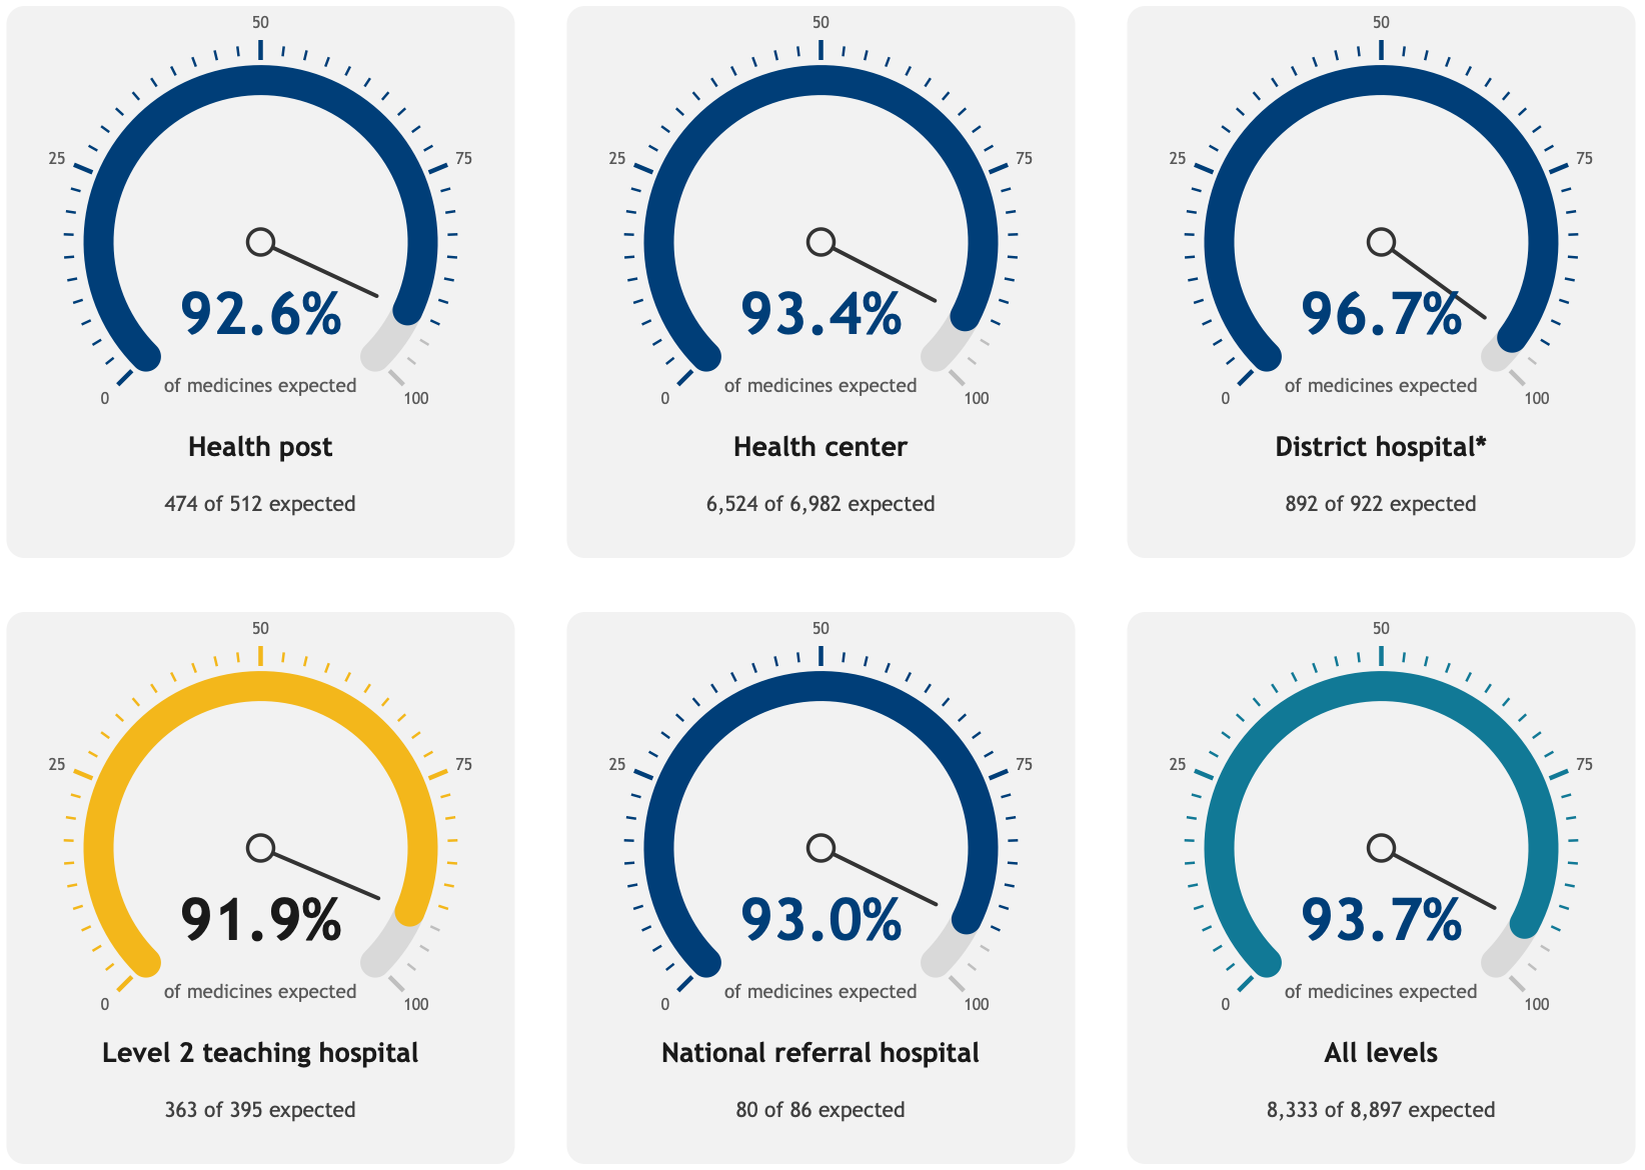
\includegraphics[width=0.84\linewidth]{gauges.png}\caption{Availability of managed products by level of care.}\end{figure}
\begin{figure}[H]\centering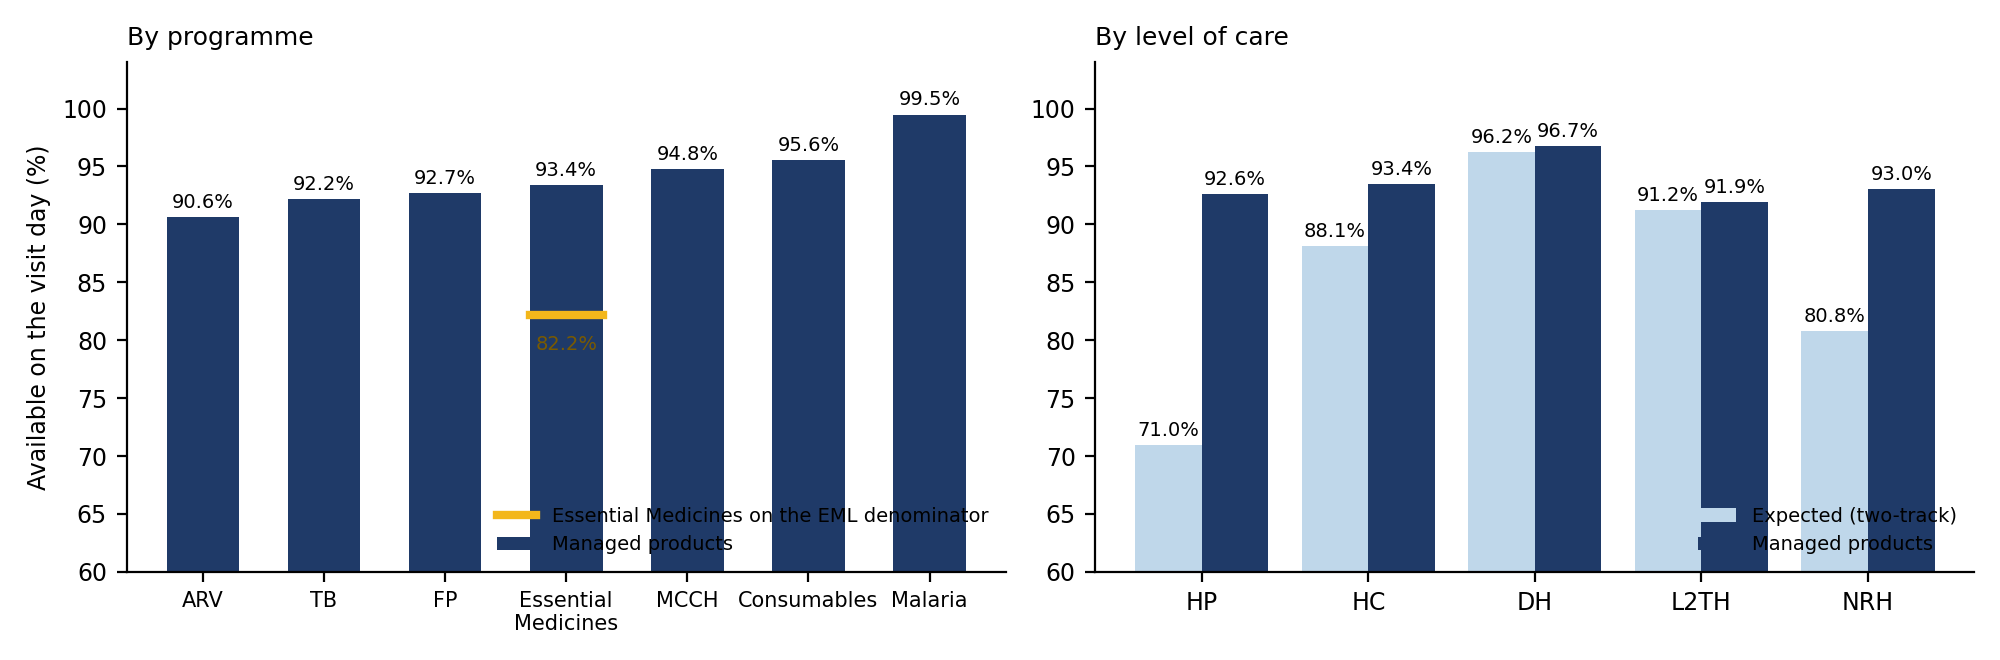
\includegraphics[width=0.96\linewidth]{d1_availability.png}\caption{Availability by programme and by level of care.}\end{figure}
{\footnotesize\setlength{\tabcolsep}{3pt}\renewcommand{\arraystretch}{1.15}
\begin{longtable}{>{\raggedright\arraybackslash}p{0.268\linewidth}>{\raggedright\arraybackslash}p{0.119\linewidth}>{\raggedright\arraybackslash}p{0.143\linewidth}>{\raggedright\arraybackslash}p{0.179\linewidth}>{\raggedright\arraybackslash}p{0.119\linewidth}>{\raggedright\arraybackslash}p{0.131\linewidth}}
\caption{Availability by level of care (expected medicines)}\\
\rowcolor{navy}\textbf{\color{white}Group} & \textbf{\color{white}Facilities} & \textbf{\color{white}Expected (denominator)} & \textbf{\color{white}EML item not managed (counted unavailable)} & \textbf{\color{white}Available} & \textbf{\color{white}AVAILABLE \%} \\
\endfirsthead
\rowcolor{navy}\textbf{\color{white}Group} & \textbf{\color{white}Facilities} & \textbf{\color{white}Expected (denominator)} & \textbf{\color{white}EML item not managed (counted unavailable)} & \textbf{\color{white}Available} & \textbf{\color{white}AVAILABLE \%} \\
\endhead
Health post & 25 & 668 & 156 & 474 & 71.0\% \\
\rowcolor{band}Health centre & 205 & 7,401 & 420 & 6,523 & 88.1\% \\
District hospital & 24 & 927 & 5 & 892 & 96.2\% \\
\rowcolor{band}Level 2 teaching hospital & 10 & 398 & 3 & 363 & 91.2\% \\
National referral hospital & 2 & 99 & 13 & 80 & 80.8\% \\
\end{longtable}}
{\footnotesize\setlength{\tabcolsep}{3pt}\renewcommand{\arraystretch}{1.15}
\begin{longtable}{>{\raggedright\arraybackslash}p{0.268\linewidth}>{\raggedright\arraybackslash}p{0.119\linewidth}>{\raggedright\arraybackslash}p{0.143\linewidth}>{\raggedright\arraybackslash}p{0.179\linewidth}>{\raggedright\arraybackslash}p{0.119\linewidth}>{\raggedright\arraybackslash}p{0.131\linewidth}}
\caption{Availability by programme (expected medicines)}\\
\rowcolor{navy}\textbf{\color{white}Group} & \textbf{\color{white}Facilities} & \textbf{\color{white}Expected (denominator)} & \textbf{\color{white}EML item not managed (counted unavailable)} & \textbf{\color{white}Available} & \textbf{\color{white}AVAILABLE \%} \\
\endfirsthead
\rowcolor{navy}\textbf{\color{white}Group} & \textbf{\color{white}Facilities} & \textbf{\color{white}Expected (denominator)} & \textbf{\color{white}EML item not managed (counted unavailable)} & \textbf{\color{white}Available} & \textbf{\color{white}AVAILABLE \%} \\
\endhead
ARV & 252 & 884 & 0.0\% & 801 & 90.6\% \\
\rowcolor{band}Consumables & 266 & 810 & 0.0\% & 774 & 95.6\% \\
Essential Medicines & 266 & 4,969 & 597 & 4,084 & 82.2\% \\
\rowcolor{band}FP & 221 & 833 & 0.0\% & 772 & 92.7\% \\
MCCH & 253 & 691 & 0.0\% & 655 & 94.8\% \\
\rowcolor{band}Malaria & 265 & 578 & 0.0\% & 575 & 99.5\% \\
TB & 240 & 727 & 0.0\% & 670 & 92.2\% \\
\end{longtable}}
{\footnotesize\setlength{\tabcolsep}{3pt}\renewcommand{\arraystretch}{1.15}
\begin{longtable}{>{\raggedright\arraybackslash}p{0.311\linewidth}>{\raggedright\arraybackslash}p{0.138\linewidth}>{\raggedright\arraybackslash}p{0.180\linewidth}>{\raggedright\arraybackslash}p{0.166\linewidth}>{\raggedright\arraybackslash}p{0.166\linewidth}}
\caption{Availability by province (expected medicines)}\\
\rowcolor{navy}\textbf{\color{white}Group} & \textbf{\color{white}Facilities} & \textbf{\color{white}Expected (denominator)} & \textbf{\color{white}Available} & \textbf{\color{white}AVAILABLE \%} \\
\endfirsthead
\rowcolor{navy}\textbf{\color{white}Group} & \textbf{\color{white}Facilities} & \textbf{\color{white}Expected (denominator)} & \textbf{\color{white}Available} & \textbf{\color{white}AVAILABLE \%} \\
\endhead
East & 65 & 2,365 & 2,087 & 88.2\% \\
\rowcolor{band}Kigali City & 26 & 938 & 813 & 86.7\% \\
North & 50 & 1,768 & 1,557 & 88.1\% \\
\rowcolor{band}South & 71 & 2,477 & 2,164 & 87.4\% \\
West & 54 & 1,945 & 1,711 & 88.0\% \\
\end{longtable}}
\begin{figure}[H]\centering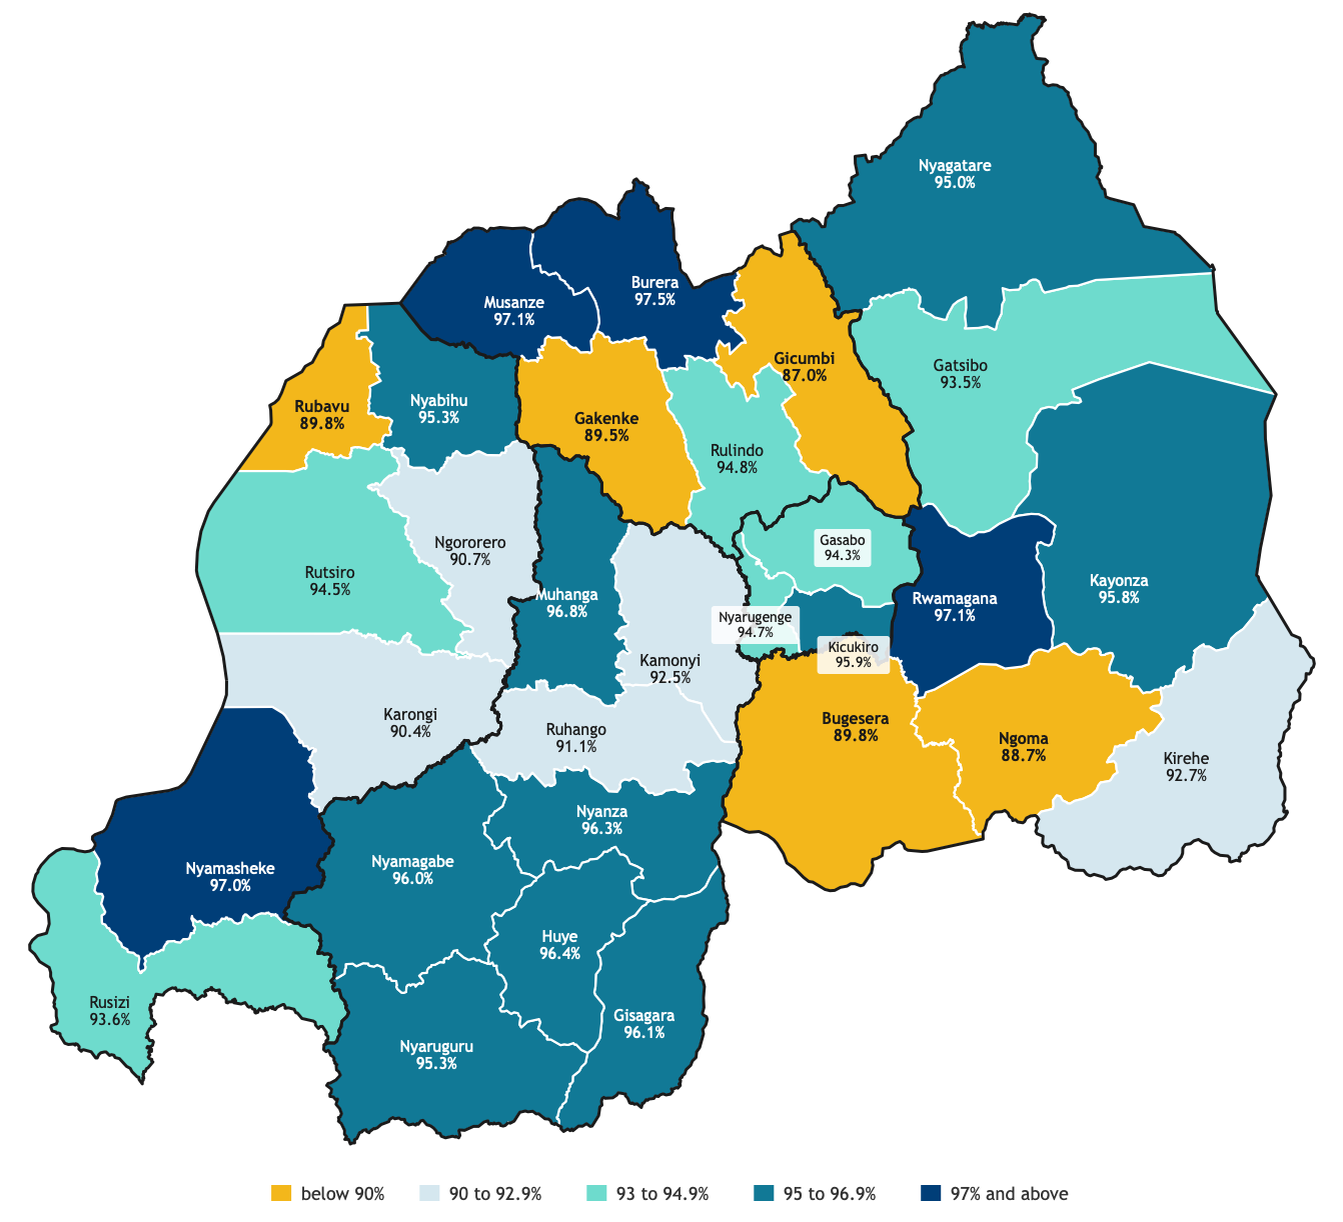
\includegraphics[width=0.66\linewidth]{map_tracer.png}\caption{Managed-product availability by district.}\end{figure}
\begin{figure}[H]\centering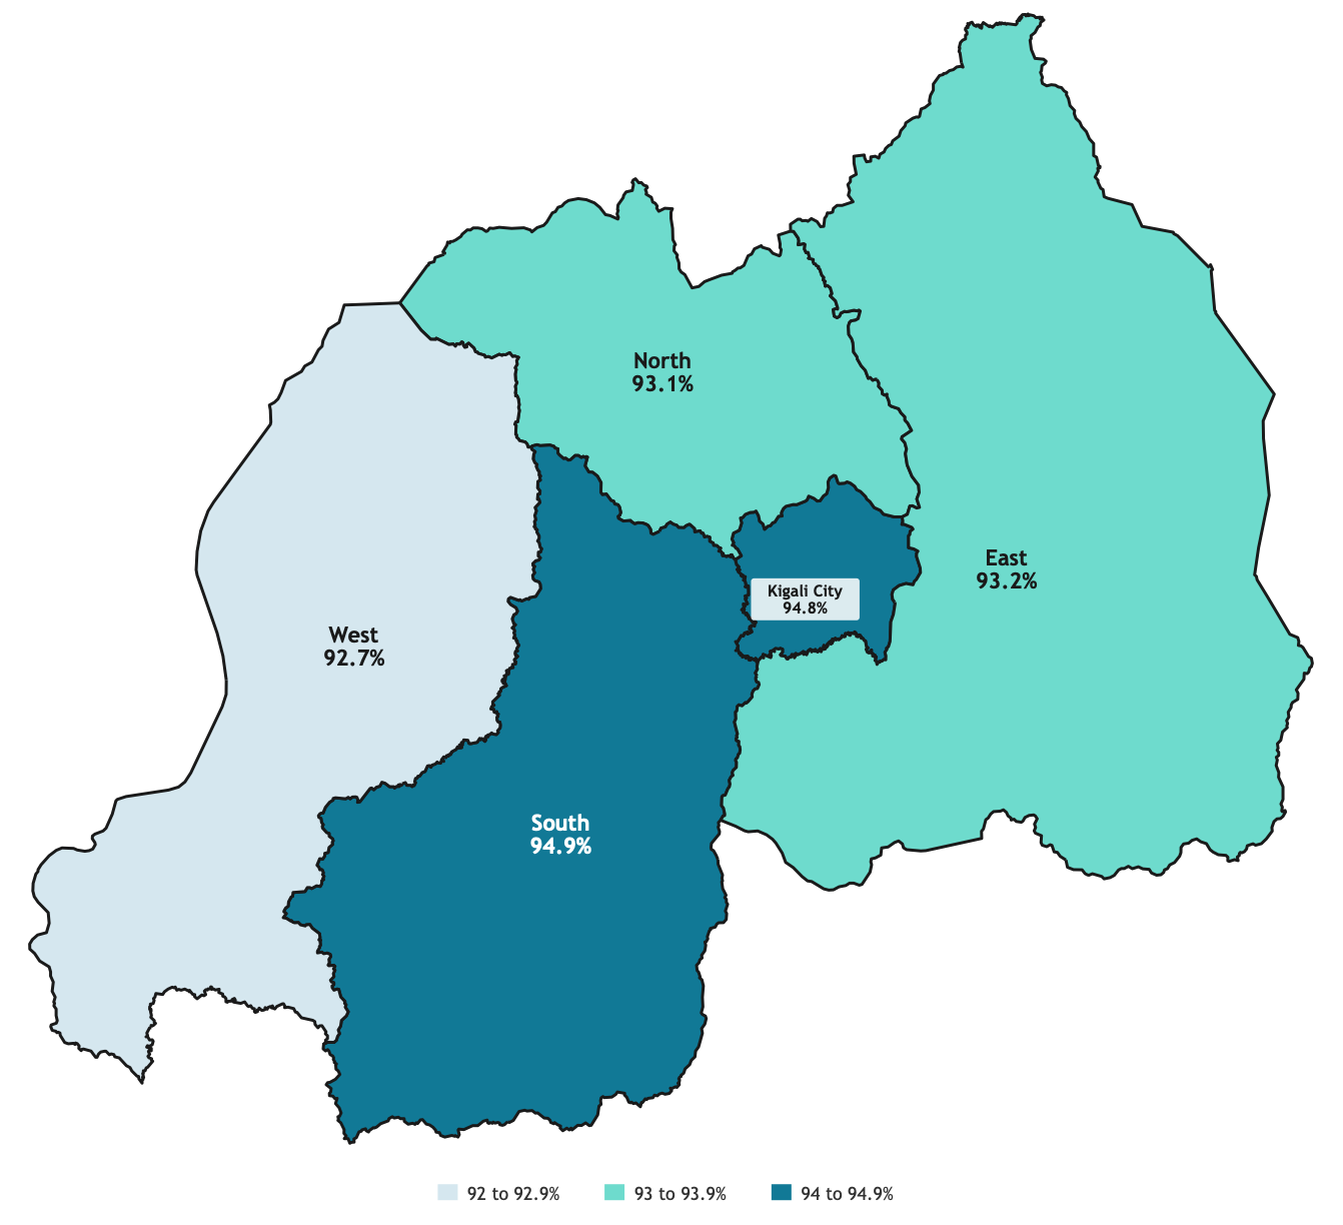
\includegraphics[width=0.54\linewidth]{map_prov.png}\caption{Managed-product availability by province.}\end{figure}
By district, Gicumbi, Ngoma, Gakenke, Rubavu and Bugesera are below 90\% on managed products; Burera, Musanze, Rwamagana and Nyamasheke are at or above 97\%.

{\footnotesize\setlength{\tabcolsep}{3pt}\renewcommand{\arraystretch}{1.15}
\begin{longtable}{>{\raggedright\arraybackslash}p{0.415\linewidth}>{\raggedright\arraybackslash}p{0.178\linewidth}>{\raggedright\arraybackslash}p{0.119\linewidth}>{\raggedright\arraybackslash}p{0.119\linewidth}>{\raggedright\arraybackslash}p{0.130\linewidth}}
\caption{The ten least available medicines (expected basis)}\\
\rowcolor{navy}\textbf{\color{white}Medicine} & \textbf{\color{white}Programme} & \textbf{\color{white}Facilities} & \textbf{\color{white}Available} & \textbf{\color{white}AVAILABLE \%} \\
\endfirsthead
\rowcolor{navy}\textbf{\color{white}Medicine} & \textbf{\color{white}Programme} & \textbf{\color{white}Facilities} & \textbf{\color{white}Available} & \textbf{\color{white}AVAILABLE \%} \\
\endhead
INSULIN HUM 100UI/ML 10MLS FAST SC INJ & Essential Medicines & 203 & 56 & 27.6\% \\
\rowcolor{band}GLICLAZIDE 60MG TAB & Essential Medicines & 262 & 117 & 44.7\% \\
BECLOMETHASONE INHALATION SOLUTION 250MCG/DOSE & Essential Medicines & 242 & 131 & 54.1\% \\
\rowcolor{band}Diclofenac Suppository & Essential Medicines & 257 & 177 & 68.9\% \\
Thiamine (all 2 strengths) & Essential Medicines & 265 & 200 & 75.5\% \\
\rowcolor{band}RIFAMP 75+ISONIAZID 50+ PYRAZINAMID150/84 & TB & 124 & 96 & 77.4\% \\
HIV-1/2  Determine HIV Early Detect  100 Tests & ARV & 250 & 195 & 78.0\% \\
\rowcolor{band}Amlodipine (all 2 strengths) & Essential Medicines & 265 & 219 & 82.6\% \\
Carbamezepine (all 2 strengths) & Essential Medicines & 265 & 222 & 83.8\% \\
\rowcolor{band}Polyglactin 910 1 coated 1/2 circle round body 37mm L:75cm & Consumables & 63 & 53 & 84.1\% \\
\end{longtable}}
{\footnotesize\setlength{\tabcolsep}{3pt}\renewcommand{\arraystretch}{1.15}
\begin{longtable}{>{\raggedright\arraybackslash}p{0.266\linewidth}>{\raggedright\arraybackslash}p{0.150\linewidth}>{\raggedright\arraybackslash}p{0.173\linewidth}>{\raggedright\arraybackslash}p{0.116\linewidth}>{\raggedright\arraybackslash}p{0.116\linewidth}>{\raggedright\arraybackslash}p{0.139\linewidth}}
\caption{The twenty facilities with the lowest expected availability}\\
\rowcolor{navy}\textbf{\color{white}Facility} & \textbf{\color{white}District} & \textbf{\color{white}Level of care} & \textbf{\color{white}Expected assessed} & \textbf{\color{white}Available} & \textbf{\color{white}FACILITY AVAILABILITY \%} \\
\endfirsthead
\rowcolor{navy}\textbf{\color{white}Facility} & \textbf{\color{white}District} & \textbf{\color{white}Level of care} & \textbf{\color{white}Expected assessed} & \textbf{\color{white}Available} & \textbf{\color{white}FACILITY AVAILABILITY \%} \\
\endhead
MBABE HP & Kicukiro & Health post & 24 & 14 & 58.3\% \\
\rowcolor{band}KIBERINKA - GAHONDO HP & Nyanza & Health post & 22 & 13 & 59.1\% \\
KIBURARA HP & Gatsibo & Health post & 27 & 16 & 59.3\% \\
\rowcolor{band}BASUMBA HP & Nyabihu & Health post & 26 & 16 & 61.5\% \\
BURUNGA HP & Karongi & Health post & 28 & 18 & 64.3\% \\
\rowcolor{band}Gatuna HP & Gicumbi & Health post & 31 & 20 & 64.5\% \\
Mahaza HP & Rulindo & Health post & 23 & 15 & 65.2\% \\
\rowcolor{band}AKAGARAMA HP & Ngoma & Health post & 29 & 19 & 65.5\% \\
Muhororo CS & Ngororero & Health centre & 38 & 25 & 65.8\% \\
\rowcolor{band}MUNAZI-SAVE HP & Gisagara & Health post & 27 & 18 & 66.7\% \\
Murara CS & Rubavu & Health centre & 27 & 18 & 66.7\% \\
\rowcolor{band}CYIBUMBA HP & Rusizi & Health post & 28 & 19 & 67.9\% \\
Buhuga HP & Gakenke & Health post & 25 & 17 & 68.0\% \\
\rowcolor{band}Kinazi CS & Ruhango & Health centre & 38 & 26 & 68.4\% \\
Busengo CS & Gakenke & Health centre & 35 & 24 & 68.6\% \\
\rowcolor{band}GAKERI HP & Rutsiro & Health post & 23 & 16 & 69.6\% \\
Kamanyana HP & Burera & Health post & 33 & 23 & 69.7\% \\
\rowcolor{band}Rubaya (gicumbi) CS & Gicumbi & Health centre & 38 & 27 & 71.1\% \\
IKIZERE-MUREHE HP & Rwamagana & Health post & 28 & 20 & 71.4\% \\
\rowcolor{band}BWIZA HP & Kayonza & Health post & 29 & 21 & 72.4\% \\
\end{longtable}}
{\footnotesize\setlength{\tabcolsep}{3pt}\renewcommand{\arraystretch}{1.15}
\begin{longtable}{>{\raggedright\arraybackslash}p{0.686\linewidth}>{\raggedright\arraybackslash}p{0.274\linewidth}}
\caption{Complete basket availability}\\
\rowcolor{navy}\textbf{\color{white}Measure} & \textbf{\color{white}Value} \\
\endfirsthead
\rowcolor{navy}\textbf{\color{white}Measure} & \textbf{\color{white}Value} \\
\endhead
Facilities with a complete assessment & 266 \\
\rowcolor{band}Facilities where EVERY assessed medicine was available & 13 \\
COMPLETE BASKET AVAILABILITY & 4.9\% \\
\rowcolor{band}Facilities missing exactly one medicine & 25 \\
Facilities missing five or more & 110 \\
\end{longtable}}
Only 13 of 266 facilities (4.9\%) had every assessed medicine available; 110 were missing five or more.

{\footnotesize\setlength{\tabcolsep}{3pt}\renewcommand{\arraystretch}{1.15}
\begin{longtable}{>{\raggedright\arraybackslash}p{0.243\linewidth}>{\raggedright\arraybackslash}p{0.127\linewidth}>{\raggedright\arraybackslash}p{0.127\linewidth}>{\raggedright\arraybackslash}p{0.093\linewidth}>{\raggedright\arraybackslash}p{0.370\linewidth}}
\caption{Why medicines are not managed (coded from free text)}\\
\rowcolor{navy}\textbf{\color{white}Reason (coded from the free-text answer)} & \textbf{\color{white}Essential Medicines - authorised, not managed} & \textbf{\color{white}Programme products - not managed} & \textbf{\color{white}Total} & \textbf{\color{white}Medicines citing it most} \\
\endfirsthead
\rowcolor{navy}\textbf{\color{white}Reason (coded from the free-text answer)} & \textbf{\color{white}Essential Medicines - authorised, not managed} & \textbf{\color{white}Programme products - not managed} & \textbf{\color{white}Total} & \textbf{\color{white}Medicines citing it most} \\
\endhead
No demand / no cases / referred & 92 & 243 & 335 & RIFAMP 75+ISONIAZID 50+ PYRAZI (72), ETHAMBUTOL 100 MG TABLET (61), INSULIN HUM 100UI/ML 10MLS FAS (56) \\
\rowcolor{band}MFT zoning - another antimalarial allocated to this zone & 4 & 303 & 307 & Pyronaridine/Artesunate (all 2 (103), Dihydroartemisinin/Piperaquine (95), Arte (all 2 strengths) (84) \\
Rejected by RSSB / cost & 145 & 5 & 150 & BECLOMETHASONE INHALATION SOLU (51), Diclofenac Suppository (48), GLICLAZIDE 60MG TAB (28) \\
\rowcolor{band}Uses an alternative product & 45 & 102 & 147 & Polyglactin 910 1 coated 1/2 c (50), Chromic Catgut Dec 3.5 (2/0) P (15), Heat Stable Carbetocin Injecti (11) \\
Believed not allowed at this level & 31 & 99 & 130 & Caffeine Citrate Injection (31), Heat Stable Carbetocin Injecti (21), Tranexamic Acid Injection (12) \\
\rowcolor{band}Faith-based: no modern FP by policy & 0 & 122 & 122 & Medroxyprogesterone Acetate 15 (31), Copper-bearing intrauterine de (31), Levonorgestrel 75mg/rod, 2rod  (30) \\
New product: not yet introduced, ordered or trained & 31 & 70 & 101 & Tranexamic Acid Injection (21), Heat Stable Carbetocin Injecti (18), GLICLAZIDE 60MG TAB (11) \\
\rowcolor{band}Not used / not managed (no reason) & 19 & 72 & 91 & Tranexamic Acid Injection (11), Polyglactin 910 1 coated 1/2 c (11), Heat Stable Carbetocin Injecti (9) \\
Reported not available / not supplied & 15 & 59 & 74 & Heat Stable Carbetocin Injecti (10), Tranexamic Acid Injection (8), Polyglactin 910 1 coated 1/2 c (7) \\
\rowcolor{band}Holds another strength of the same medicine & 35 & 4 & 39 & GLICLAZIDE 60MG TAB (14), CIRPOFLOXACIN 500MG TAB (6), Amlodipine (all 2 strengths) (5) \\
Not on the facility's selection list / formulary & 11 & 27 & 38 & Heat Stable Carbetocin Injecti (4), Polyglactin 910 1 coated 1/2 c (2), Tranexamic Acid Injection (2) \\
\rowcolor{band}Service not offered here (no FP / maternity / deliveries) & 17 & 18 & 35 & GLICLAZIDE 60MG TAB (5), BECLOMETHASONE INHALATION SOLU (4), Amlodipine (all 2 strengths) (3) \\
Other & 46 & 40 & 86 & Polyglactin 910 1 coated 1/2 c (13), INSULIN HUM 100UI/ML 10MLS FAS (12), RIFAMP 75+ISONIAZID 50+ PYRAZI (9) \\
\rowcolor{band}(no reason recorded) & 106 & 850 & 956 & Caffeine Citrate Injection (160), Heat Stable Carbetocin Injecti (133), Polyglactin 910 1 coated 1/2 c (74) \\
TOTAL not managed & 597 & 2,014 & 2,611 &  \\
\end{longtable}}
The main reasons are no demand or referral, MFT zoning (policy), rejection by RSSB or cost, and use of an alternative product. Faith-based facilities do not provide modern family planning by policy (122 pairs).

\section{Inferential findings}
\subsection{Factors associated with availability}
{\footnotesize\setlength{\tabcolsep}{3pt}\renewcommand{\arraystretch}{1.15}
\begin{longtable}{>{\raggedright\arraybackslash}p{0.565\linewidth}>{\raggedright\arraybackslash}p{0.248\linewidth}>{\raggedright\arraybackslash}p{0.147\linewidth}}
\caption{Model 1: adjusted odds ratios for availability of a managed medicine}\\
\rowcolor{navy}\textbf{\color{white}Factor} & \textbf{\color{white}Adjusted OR (95\% CI)} & \textbf{\color{white}p} \\
\endfirsthead
\rowcolor{navy}\textbf{\color{white}Factor} & \textbf{\color{white}Adjusted OR (95\% CI)} & \textbf{\color{white}p} \\
\endhead
Level: District hospital (ref. Health centre) & 3.29 (1.78-6.08) & $<$0.001 \\
\rowcolor{band}Level: Health post (ref. Health centre) & 1.70 (0.70-4.15) & 0.241 \\
Level: Referral / teaching (ref. Health centre) & 1.18 (0.66-2.11) & 0.569 \\
\rowcolor{band}Management: Faith-based (ref. Government) & 1.41 (1.03-1.92) & 0.030 \\
Management: PPP (ref. Government) & 0.49 (0.24-1.01) & 0.052 \\
\rowcolor{band}Province: East (ref. Kigali City) & 0.78 (0.55-1.11) & 0.172 \\
Province: North (ref. Kigali City) & 0.71 (0.48-1.07) & 0.103 \\
\rowcolor{band}Province: South (ref. Kigali City) & 0.92 (0.60-1.40) & 0.694 \\
Province: West (ref. Kigali City) & 0.60 (0.39-0.93) & 0.021 \\
\rowcolor{band}Programme: ARV (ref. Essential Medicines) & 0.67 (0.51-0.87) & 0.003 \\
Programme: Consumables (ref. Essential Medicines) & 1.53 (1.09-2.14) & 0.013 \\
\rowcolor{band}Programme: FP (ref. Essential Medicines) & 0.98 (0.74-1.30) & 0.882 \\
Programme: MCCH (ref. Essential Medicines) & 1.24 (0.85-1.82) & 0.264 \\
\rowcolor{band}Programme: Malaria (ref. Essential Medicines) & 13.89 (4.42-43.62) & $<$0.001 \\
Programme: TB (ref. Essential Medicines) & 0.81 (0.59-1.13) & 0.212 \\
\rowcolor{band}Setting: urban (ref. rural) & 1.02 (0.73-1.41) & 0.929 \\
Main digital system: Medisoft (ref. eLMIS) & 0.88 (0.56-1.38) & 0.576 \\
\rowcolor{band}Main digital system: OpenMRS (ref. eLMIS) & 0.60 (0.35-1.02) & 0.059 \\
Main digital system: Other / none (ref. eLMIS) & 0.91 (0.54-1.53) & 0.718 \\
\rowcolor{band}Main digital system: eBuzima (ref. eLMIS) & 1.00 (0.69-1.45) & 0.986 \\
Facility fill rate (per +10 points) & 0.99 (0.88-1.12) & 0.904 \\
\rowcolor{band}Facility record accuracy (per +10 points) & 0.97 (0.94-1.01) & 0.128 \\
\multicolumn{3}{p{0.96\linewidth}}{\scriptsize\itshape\color{gray} Outcome: managed medicine available on the visit day. n = 8,861 pairs, 265 facilities.}\\
\end{longtable}}
\begin{figure}[H]\centering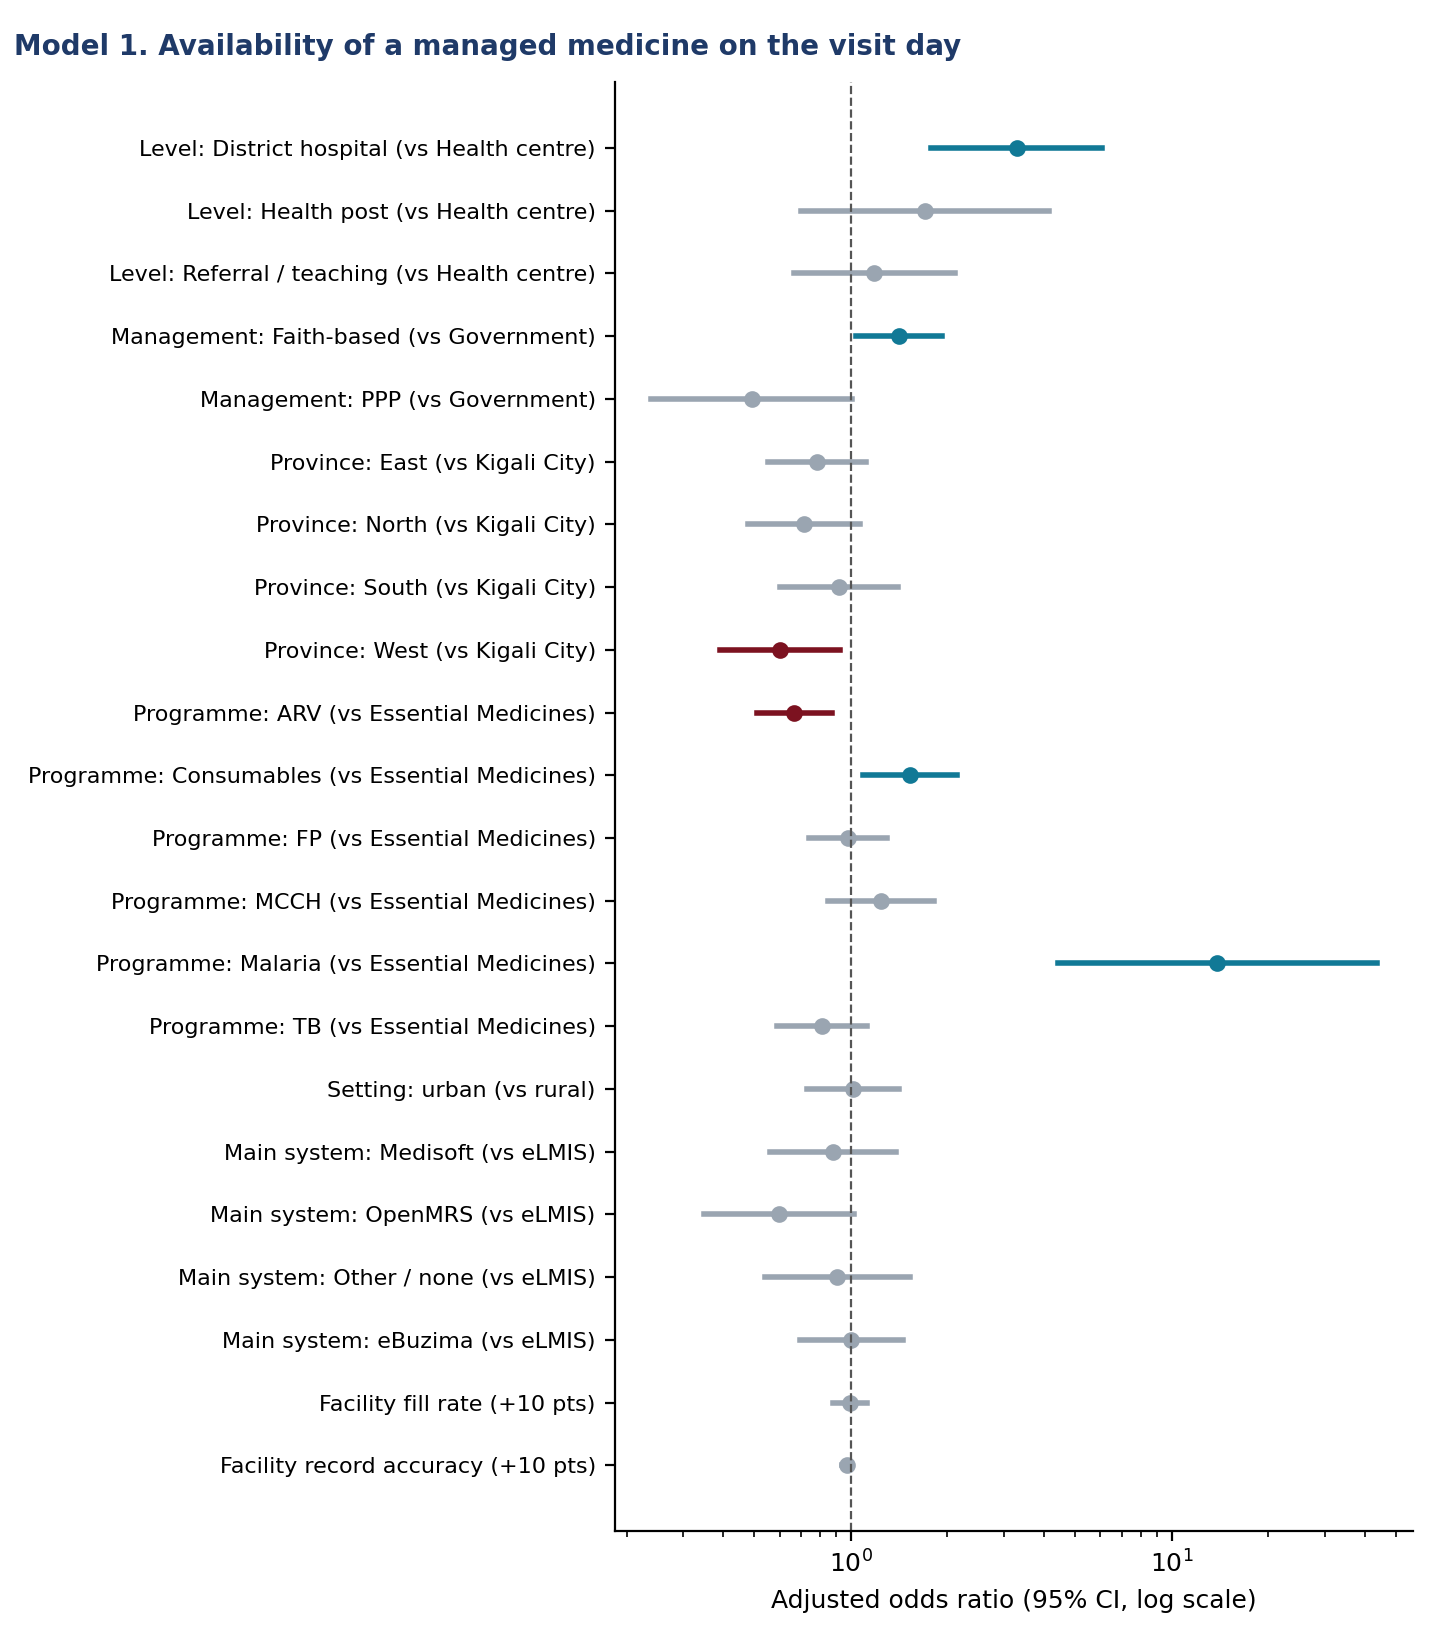
\includegraphics[width=0.78\linewidth]{fig_forest_availability.png}\caption{Adjusted odds ratios for availability.}\end{figure}
\textbf{Interpretation.} With level, ownership, location, programme and system held constant, district hospitals are about three times as likely as health centres to have a managed medicine on the shelf (OR 3.29 (1.78-6.08)). Faith-based facilities do better than government ones (OR 1.41 (1.03-1.92)), as in Malawi [Mohan 2024]. The West is the only province significantly below Kigali City (OR 0.60 (0.39-0.93)). Among programmes, malaria commodities are almost always present (OR 13.89 (4.42-43.62)) and ARV products least (OR 0.67 (0.51-0.87)), consistent with the nationwide ARV stock-outs on the dashboard. Neither the facility's fill rate, its record accuracy, its digital system nor urban setting predicts availability once these are accounted for: availability is driven more by what is in the national pipeline for a given medicine than by facility traits.

\chapter{Inventory record accuracy and stock adequacy (objective 2)}
\section{Descriptive findings: record accuracy}
Among 8,856 records naming a digital system, the physical count equalled the system count in 56.1\%. Accuracy rises with level of care, from 38.1\% at health posts to 85.1\% at district hospitals.

\begin{figure}[H]\centering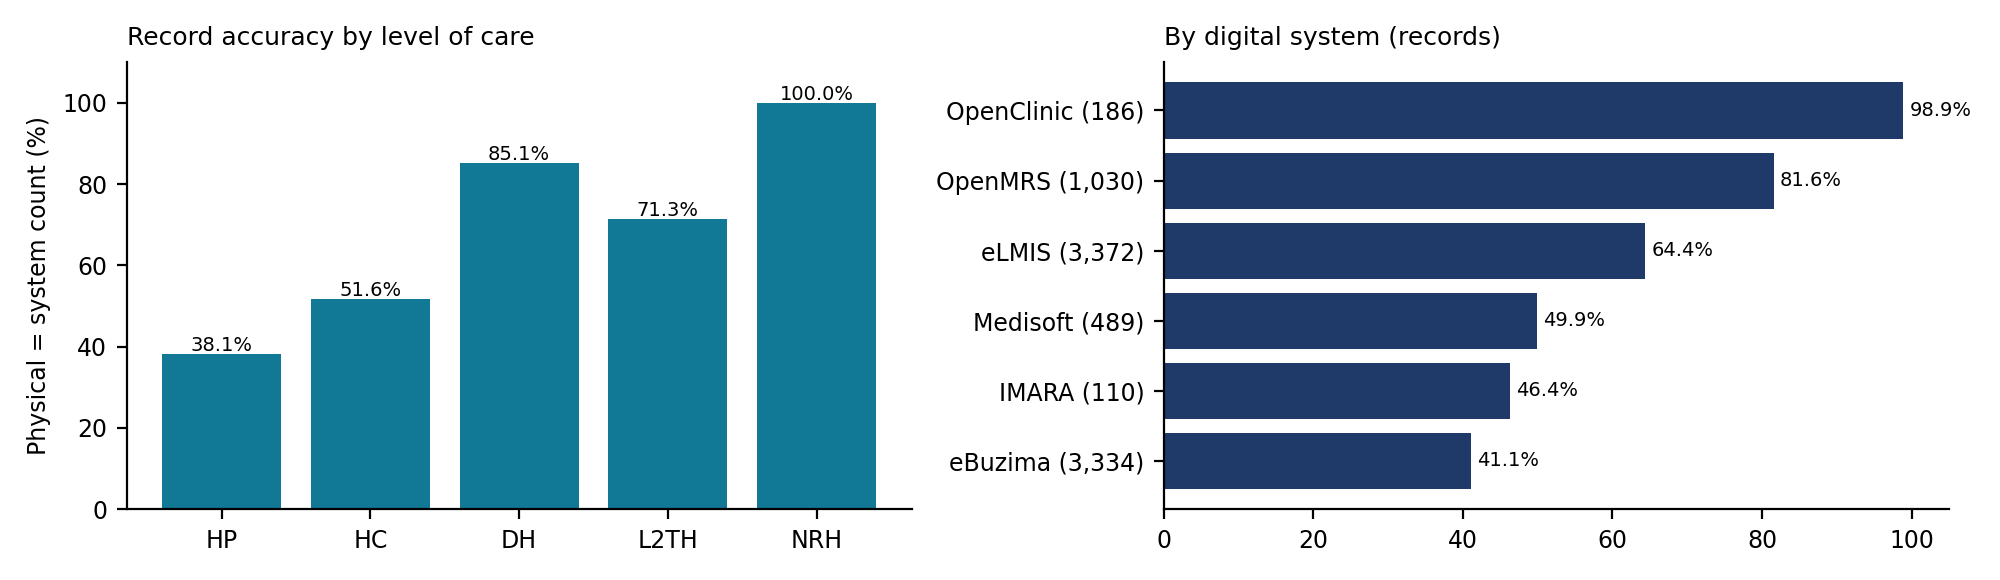
\includegraphics[width=0.96\linewidth]{d3_accuracy.png}\caption{Inventory record accuracy by level of care and by digital system.}\end{figure}
{\footnotesize\setlength{\tabcolsep}{3pt}\renewcommand{\arraystretch}{1.15}
\begin{longtable}{>{\raggedright\arraybackslash}p{0.343\linewidth}>{\raggedright\arraybackslash}p{0.206\linewidth}>{\raggedright\arraybackslash}p{0.206\linewidth}>{\raggedright\arraybackslash}p{0.206\linewidth}}
\caption{Inventory record accuracy by level of care}\\
\rowcolor{navy}\textbf{\color{white}Level of care} & \textbf{\color{white}Rows counted} & \textbf{\color{white}Exact match} & \textbf{\color{white}EXACT ACCURACY \%} \\
\endfirsthead
\rowcolor{navy}\textbf{\color{white}Level of care} & \textbf{\color{white}Rows counted} & \textbf{\color{white}Exact match} & \textbf{\color{white}EXACT ACCURACY \%} \\
\endhead
Health post & 404 & 154 & 38.1\% \\
\rowcolor{band}Health centre & 6,973 & 3,599 & 51.6\% \\
District hospital & 989 & 842 & 85.1\% \\
\rowcolor{band}Level 2 teaching hospital & 411 & 293 & 71.3\% \\
National referral hospital & 79 & 79 & 100.0\% \\
\end{longtable}}
{\footnotesize\setlength{\tabcolsep}{3pt}\renewcommand{\arraystretch}{1.15}
\begin{longtable}{>{\raggedright\arraybackslash}p{0.343\linewidth}>{\raggedright\arraybackslash}p{0.206\linewidth}>{\raggedright\arraybackslash}p{0.206\linewidth}>{\raggedright\arraybackslash}p{0.206\linewidth}}
\caption{Inventory record accuracy by province}\\
\rowcolor{navy}\textbf{\color{white}Group} & \textbf{\color{white}Facilities} & \textbf{\color{white}Observations} & \textbf{\color{white}Numerator} \\
\endfirsthead
\rowcolor{navy}\textbf{\color{white}Group} & \textbf{\color{white}Facilities} & \textbf{\color{white}Observations} & \textbf{\color{white}Numerator} \\
\endhead
Kigali City & 25 & 847 & 356 \\
\rowcolor{band}South & 70 & 2,310 & 1,182 \\
North & 48 & 1,659 & 902 \\
\rowcolor{band}East & 63 & 2,208 & 1,303 \\
West & 54 & 1,832 & 1,224 \\
\end{longtable}}
{\footnotesize\setlength{\tabcolsep}{3pt}\renewcommand{\arraystretch}{1.15}
\begin{longtable}{>{\raggedright\arraybackslash}p{0.343\linewidth}>{\raggedright\arraybackslash}p{0.206\linewidth}>{\raggedright\arraybackslash}p{0.206\linewidth}>{\raggedright\arraybackslash}p{0.206\linewidth}}
\caption{Inventory record accuracy by management type}\\
\rowcolor{navy}\textbf{\color{white}Group} & \textbf{\color{white}Facilities} & \textbf{\color{white}Observations} & \textbf{\color{white}Numerator} \\
\endfirsthead
\rowcolor{navy}\textbf{\color{white}Group} & \textbf{\color{white}Facilities} & \textbf{\color{white}Observations} & \textbf{\color{white}Numerator} \\
\endhead
PPP & 21 & 431 & 147 \\
\rowcolor{band}Government & 167 & 5,936 & 3,286 \\
Faith based facility based & 71 & 2,456 & 1,505 \\
\rowcolor{band}(not recorded) & 1 & 33 & 29 \\
\end{longtable}}
\section{Descriptive findings: stock adequacy}
{\footnotesize\setlength{\tabcolsep}{3pt}\renewcommand{\arraystretch}{1.15}
\begin{longtable}{>{\raggedright\arraybackslash}p{0.209\linewidth}>{\raggedright\arraybackslash}p{0.424\linewidth}>{\raggedright\arraybackslash}p{0.170\linewidth}>{\raggedright\arraybackslash}p{0.157\linewidth}}
\caption{Stock status of managed products (months of stock)}\\
\rowcolor{navy}\textbf{\color{white}Stock category} & \textbf{\color{white}Definition} & \textbf{\color{white}Observations} & \textbf{\color{white}\% of base} \\
\endfirsthead
\rowcolor{navy}\textbf{\color{white}Stock category} & \textbf{\color{white}Definition} & \textbf{\color{white}Observations} & \textbf{\color{white}\% of base} \\
\endhead
Stocked out & not available on the visit day & 591 & 7.0\% \\
\rowcolor{band}Understock & on the shelf, under 1 month of stock & 1,889 & 22.3\% \\
Adequate stock & 1 to 2 months (1 to 3 at teaching and referral hospitals) & 2,081 & 24.6\% \\
\rowcolor{band}Overstock & more than 2 months (3 at teaching and referral hospitals) & 3,913 & 46.2\% \\
\end{longtable}}
\begin{figure}[H]\centering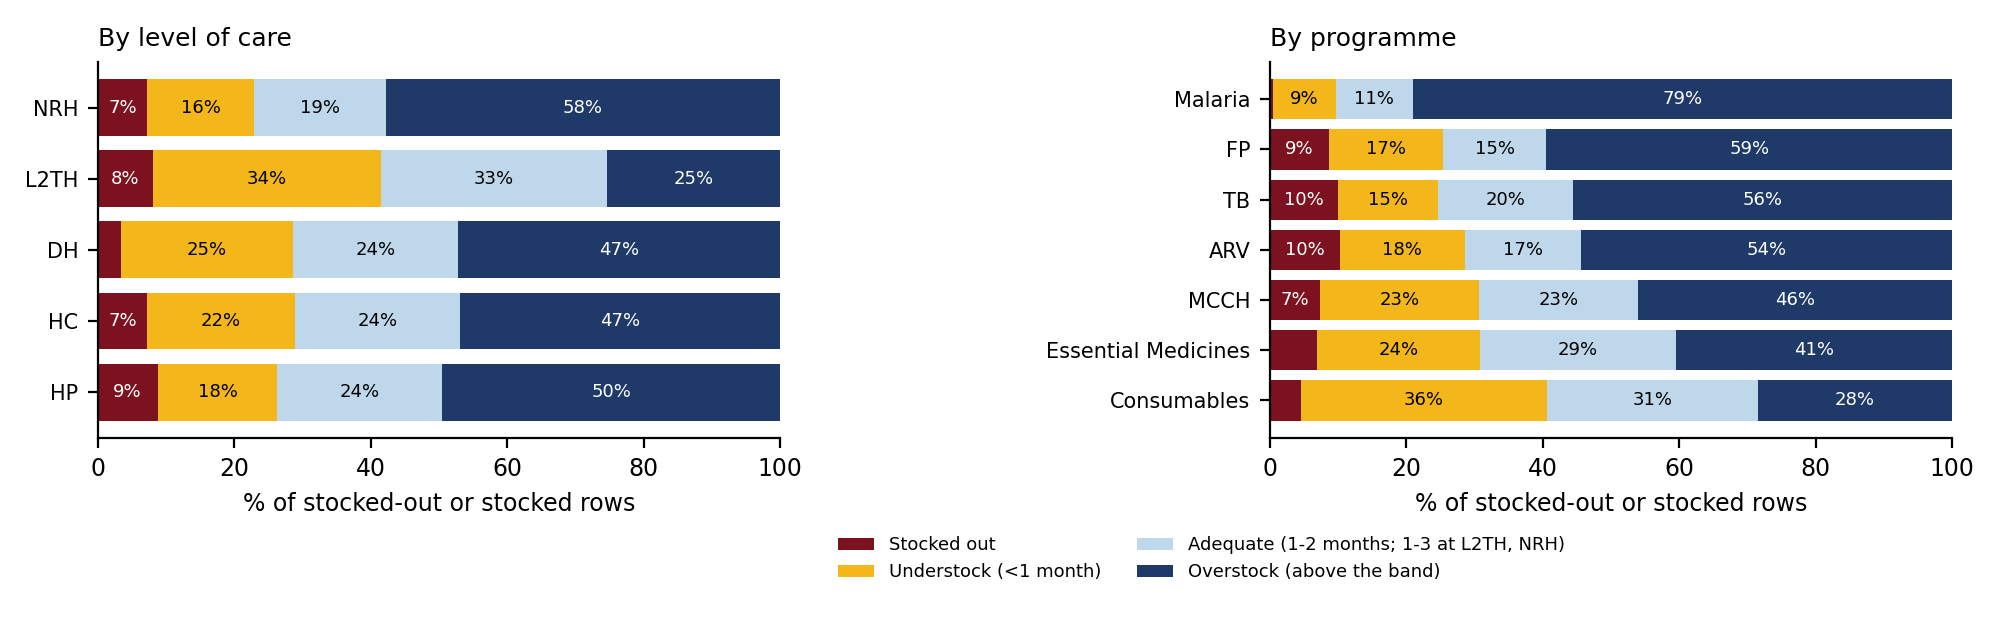
\includegraphics[width=0.96\linewidth]{d2_adequacy.png}\caption{Stock adequacy by level of care and by programme.}\end{figure}
Overstock dominates: 46.2\% of items held more than the maximum (two months; three at level 2 teaching and national referral hospitals), rising to 79\% for malaria products. With the wider band, 33.0\% of items at level 2 teaching hospitals are adequately stocked. Understock affects 22.3\%, and 928 items (49\% of the understocked) were at or below 0.5 months, the emergency order point.

\section{Inferential findings}
\subsection{Factors associated with record accuracy}
{\footnotesize\setlength{\tabcolsep}{3pt}\renewcommand{\arraystretch}{1.15}
\begin{longtable}{>{\raggedright\arraybackslash}p{0.565\linewidth}>{\raggedright\arraybackslash}p{0.248\linewidth}>{\raggedright\arraybackslash}p{0.147\linewidth}}
\caption{Model 3: adjusted odds ratios for an exact record match}\\
\rowcolor{navy}\textbf{\color{white}Factor} & \textbf{\color{white}Adjusted OR (95\% CI)} & \textbf{\color{white}p} \\
\endfirsthead
\rowcolor{navy}\textbf{\color{white}Factor} & \textbf{\color{white}Adjusted OR (95\% CI)} & \textbf{\color{white}p} \\
\endhead
Digital system: Medisoft (ref. eLMIS) & 0.36 (0.15-0.83) & 0.017 \\
\rowcolor{band}Digital system: OpenMRS (ref. eLMIS) & 0.48 (0.15-1.54) & 0.218 \\
Digital system: Other (ref. eLMIS) & 0.50 (0.19-1.34) & 0.168 \\
\rowcolor{band}Digital system: eBuzima (ref. eLMIS) & 0.26 (0.15-0.46) & $<$0.001 \\
Level: District hospital (ref. Health centre) & 5.91 (2.21-15.84) & $<$0.001 \\
\rowcolor{band}Level: Health post (ref. Health centre) & 2.36 (0.50-11.18) & 0.279 \\
Level: Referral / teaching (ref. Health centre) & 2.64 (0.59-11.86) & 0.207 \\
\rowcolor{band}Management: Faith-based (ref. Government) & 1.00 (0.61-1.63) & 0.994 \\
Management: PPP (ref. Government) & 0.16 (0.04-0.73) & 0.018 \\
\rowcolor{band}Province: East (ref. Kigali City) & 2.00 (1.08-3.71) & 0.027 \\
Province: North (ref. Kigali City) & 1.63 (0.82-3.26) & 0.163 \\
\rowcolor{band}Province: South (ref. Kigali City) & 0.74 (0.36-1.53) & 0.412 \\
Province: West (ref. Kigali City) & 1.02 (0.45-2.32) & 0.956 \\
\rowcolor{band}Programme: ARV (ref. Essential Medicines) & 1.17 (0.96-1.41) & 0.115 \\
Programme: Consumables (ref. Essential Medicines) & 0.82 (0.72-0.94) & 0.004 \\
\rowcolor{band}Programme: FP (ref. Essential Medicines) & 0.87 (0.72-1.05) & 0.155 \\
Programme: MCCH (ref. Essential Medicines) & 1.13 (0.93-1.38) & 0.212 \\
\rowcolor{band}Programme: Malaria (ref. Essential Medicines) & 1.01 (0.85-1.21) & 0.900 \\
Programme: TB (ref. Essential Medicines) & 0.98 (0.80-1.20) & 0.827 \\
\multicolumn{3}{p{0.96\linewidth}}{\scriptsize\itshape\color{gray} Outcome: physical count equals system count. n = 8,822 records.}\\
\end{longtable}}
\begin{figure}[H]\centering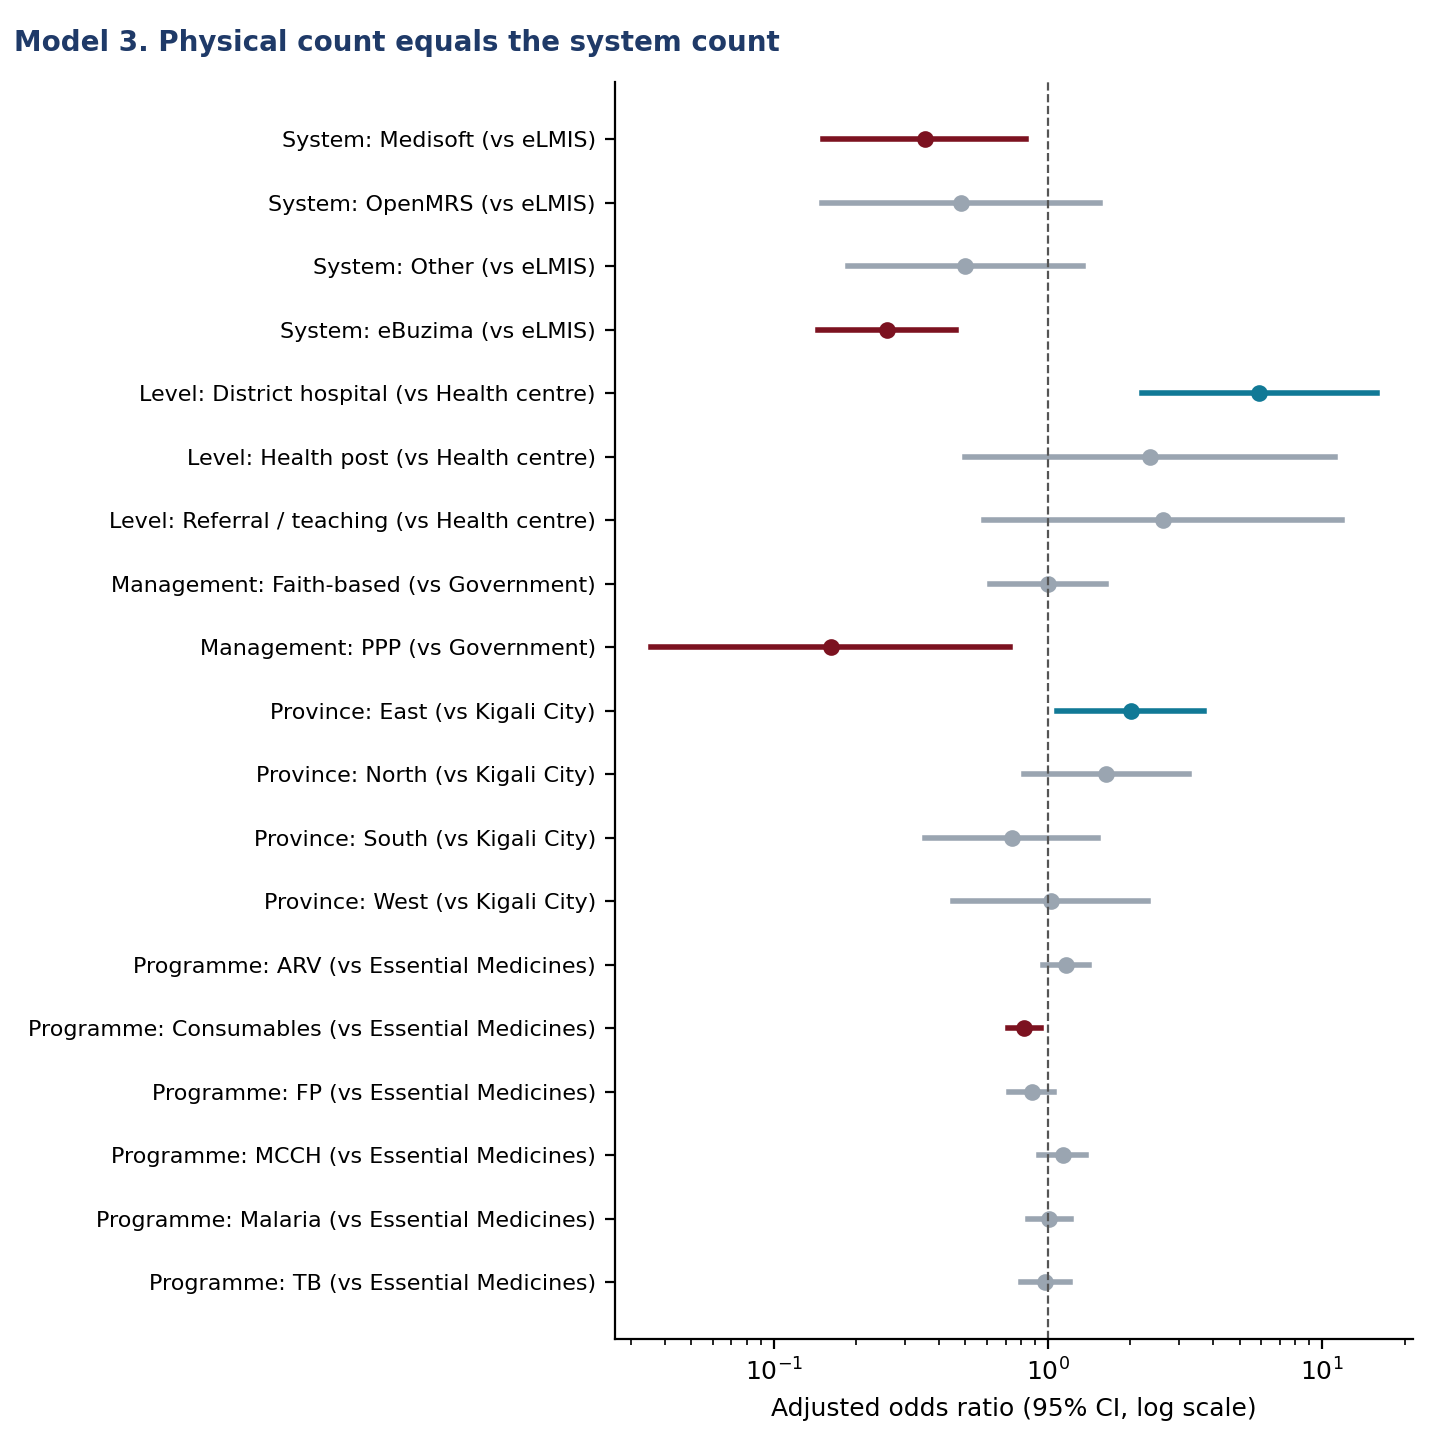
\includegraphics[width=0.78\linewidth]{fig_forest_accuracy.png}\caption{Adjusted odds ratios for exact record match.}\end{figure}
\textbf{Interpretation.} Records kept in eBuzima matched the shelf far less often than eLMIS records (OR 0.26 (0.15-0.46)), as did Medisoft (OR 0.36 (0.15-0.83)), after level and location are held constant. eBuzima is a point-of-care system whose stock module depends on dispensing being recorded for every patient, which the data-collector feedback says is often not done. District hospitals are much more accurate than health centres (OR 5.91 (2.21-15.84)) and PPP facilities much less (OR 0.16 (0.04-0.73)). The Rwandan QMIA reached 85\% accuracy by 2019 [Kigenza 2023]. Definitions may differ, but today's 56\% suggests that some of that gain has been lost; the eBuzima result points to the transition of health centres to point-of-care systems as one likely reason.

\chapter{Medicine consumption}
Consumption (June-August) underpins quantification and the stock adequacy and lost-sales estimates. Average monthly consumption (AMC) is the mean of the months with a value.

\begin{figure}[H]\centering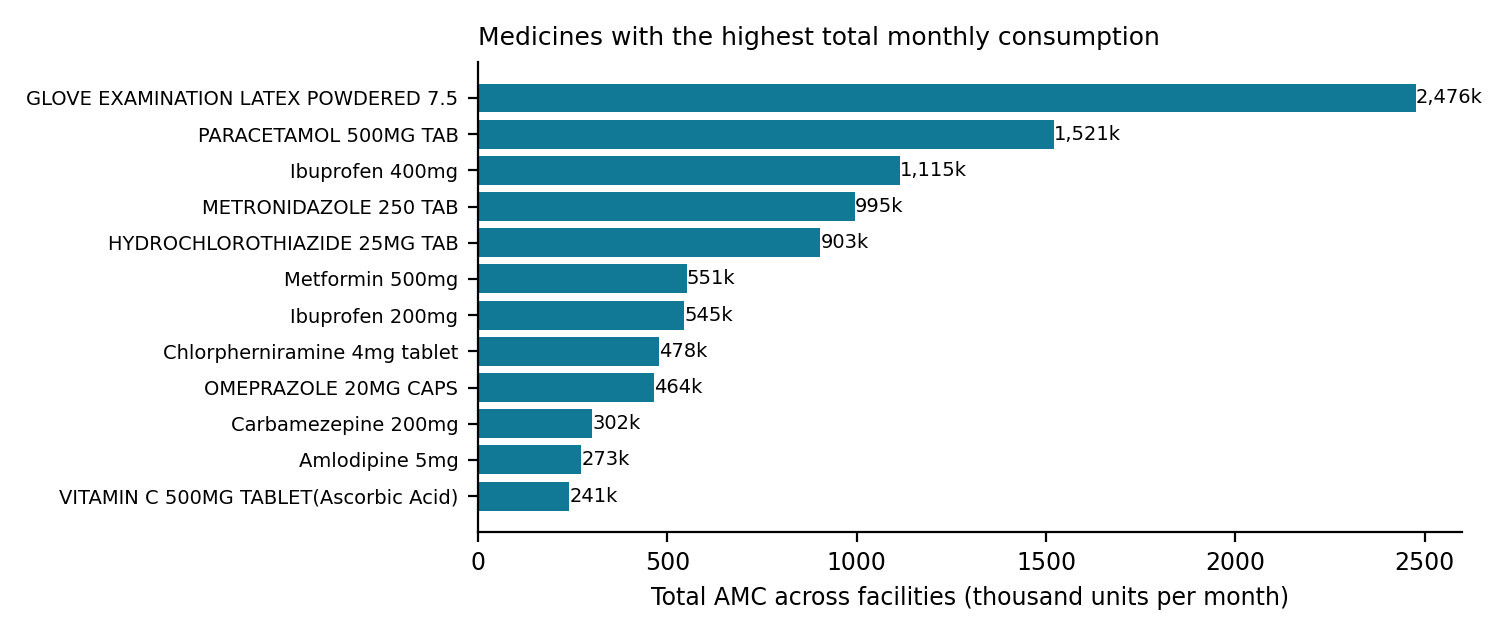
\includegraphics[width=0.78\linewidth]{d7_consumption.png}\caption{Medicines with the highest total AMC across facilities.}\end{figure}
{\footnotesize\setlength{\tabcolsep}{3pt}\renewcommand{\arraystretch}{1.15}
\begin{longtable}{>{\raggedright\arraybackslash}p{0.327\linewidth}>{\raggedright\arraybackslash}p{0.164\linewidth}>{\raggedright\arraybackslash}p{0.098\linewidth}>{\raggedright\arraybackslash}p{0.131\linewidth}>{\raggedright\arraybackslash}p{0.120\linewidth}>{\raggedright\arraybackslash}p{0.120\linewidth}}
\caption{Average monthly consumption: the twelve highest}\\
\rowcolor{navy}\textbf{\color{white}Medicine} & \textbf{\color{white}Programme} & \textbf{\color{white}Facilities} & \textbf{\color{white}Total AMC} & \textbf{\color{white}Mean AMC} & \textbf{\color{white}Median AMC} \\
\endfirsthead
\rowcolor{navy}\textbf{\color{white}Medicine} & \textbf{\color{white}Programme} & \textbf{\color{white}Facilities} & \textbf{\color{white}Total AMC} & \textbf{\color{white}Mean AMC} & \textbf{\color{white}Median AMC} \\
\endhead
GLOVE EXAMINATION LATEX POWDERED 7.5 & Consumables & 264 & 2,475,847.7 & 9,378.2 & 2,450 \\
\rowcolor{band}PARACETAMOL 500MG TAB & Essential Medicines & 262 & 1,520,935.3 & 5,805.1 & 4,170 \\
Ibuprofen 400mg & Essential Medicines & 221 & 1,114,501.7 & 5,043 & 4,166.7 \\
\rowcolor{band}METRONIDAZOLE 250 TAB & Essential Medicines & 262 & 994,510.7 & 3,795.8 & 3,333.3 \\
HYDROCHLOROTHIAZIDE 25MG TAB & Essential Medicines & 234 & 903,044.7 & 3,859.2 & 3,333.3 \\
\rowcolor{band}Metformin 500mg & Essential Medicines & 232 & 550,715.3 & 2,373.8 & 1,083.3 \\
Ibuprofen 200mg & Essential Medicines & 220 & 545,211 & 2,478.2 & 1,666.7 \\
\rowcolor{band}Chlorpherniramine 4mg tablet & Essential Medicines & 264 & 477,894.3 & 1,810.2 & 1,666.7 \\
OMEPRAZOLE 20MG CAPS & Essential Medicines & 250 & 464,249.7 & 1,857 & 600 \\
\rowcolor{band}Carbamezepine 200mg & Essential Medicines & 233 & 301,621.3 & 1,294.5 & 1,000 \\
Amlodipine 5mg & Essential Medicines & 191 & 272,851 & 1,428.5 & 866.7 \\
\rowcolor{band}VITAMIN C 500MG TABLET(Ascorbic Acid) & Essential Medicines & 259 & 240,863.7 & 930 & 766.7 \\
\end{longtable}}
{\footnotesize\setlength{\tabcolsep}{3pt}\renewcommand{\arraystretch}{1.15}
\begin{longtable}{>{\raggedright\arraybackslash}p{0.316\linewidth}>{\raggedright\arraybackslash}p{0.189\linewidth}>{\raggedright\arraybackslash}p{0.152\linewidth}>{\raggedright\arraybackslash}p{0.152\linewidth}>{\raggedright\arraybackslash}p{0.152\linewidth}}
\caption{Consumption trend, August against June}\\
\rowcolor{navy}\textbf{\color{white}Group} & \textbf{\color{white}Pairs with June consumption} & \textbf{\color{white}TREND RATIO} & \textbf{\color{white}Pairs rising} & \textbf{\color{white}Pairs falling} \\
\endfirsthead
\rowcolor{navy}\textbf{\color{white}Group} & \textbf{\color{white}Pairs with June consumption} & \textbf{\color{white}TREND RATIO} & \textbf{\color{white}Pairs rising} & \textbf{\color{white}Pairs falling} \\
\endhead
Health post & 424 & 0.75 & 107 & 246 \\
\rowcolor{band}Health centre & 5,383 & 0.85 & 1,624 & 2,966 \\
District hospital & 782 & 0.82 & 241 & 464 \\
\rowcolor{band}Level 2 teaching hospital & 335 & 0.80 & 88 & 211 \\
National referral hospital & 72 & 0.82 & 21 & 41 \\
\end{longtable}}
{\footnotesize\setlength{\tabcolsep}{3pt}\renewcommand{\arraystretch}{1.15}
\begin{longtable}{>{\raggedright\arraybackslash}p{0.272\linewidth}>{\raggedright\arraybackslash}p{0.181\linewidth}>{\raggedright\arraybackslash}p{0.181\linewidth}>{\raggedright\arraybackslash}p{0.157\linewidth}>{\raggedright\arraybackslash}p{0.169\linewidth}}
\caption{Non-moving medicines (zero consumption in all three months)}\\
\rowcolor{navy}\textbf{\color{white}Level of care} & \textbf{\color{white}Pairs with complete data} & \textbf{\color{white}Zero in all three months} & \textbf{\color{white}NON-MOVING RATE} & \textbf{\color{white}Of those, held in stock} \\
\endfirsthead
\rowcolor{navy}\textbf{\color{white}Level of care} & \textbf{\color{white}Pairs with complete data} & \textbf{\color{white}Zero in all three months} & \textbf{\color{white}NON-MOVING RATE} & \textbf{\color{white}Of those, held in stock} \\
\endhead
Health post & 555 & 94 & 16.9\% & 65 \\
\rowcolor{band}Health centre & 7,517 & 1,128 & 15.0\% & 931 \\
District hospital & 1,025 & 118 & 11.5\% & 107 \\
\rowcolor{band}Level 2 teaching hospital & 445 & 53 & 11.9\% & 48 \\
National referral hospital & 86 & 4 & 4.7\% & 3 \\
\rowcolor{band}ALL LEVELS & 9,628 & 1,397 & 14.5\% & 1,154 \\
\end{longtable}}
{\footnotesize\setlength{\tabcolsep}{3pt}\renewcommand{\arraystretch}{1.15}
\begin{longtable}{>{\raggedright\arraybackslash}p{0.070\linewidth}>{\raggedright\arraybackslash}p{0.445\linewidth}>{\raggedright\arraybackslash}p{0.199\linewidth}>{\raggedright\arraybackslash}p{0.117\linewidth}>{\raggedright\arraybackslash}p{0.129\linewidth}}
\caption{Consumption value concentration (ABC analysis): the ten largest}\\
\rowcolor{navy}\textbf{\color{white}Rank} & \textbf{\color{white}Medicine} & \textbf{\color{white}Consumption value (RWF)} & \textbf{\color{white}Share} & \textbf{\color{white}CUMULATIVE} \\
\endfirsthead
\rowcolor{navy}\textbf{\color{white}Rank} & \textbf{\color{white}Medicine} & \textbf{\color{white}Consumption value (RWF)} & \textbf{\color{white}Share} & \textbf{\color{white}CUMULATIVE} \\
\endhead
1 & GLOVE EXAMINATION LATEX POWDERED 7.5 & 343,330,748 & 24.0\% & 24.0\% \\
\rowcolor{band}2 & SODIUM CHLORIDE 0.9\% SOLUTION INJ/INFUSION & 204,754,243 & 14.3\% & 38.4\% \\
3 & BECLOMETHASONE INHALATION SOLUTION 250MCG/DOSE & 115,848,008 & 8.1\% & 46.5\% \\
\rowcolor{band}4 & Caffeine Citrate Injection & 76,003,115 & 5.3\% & 51.8\% \\
5 & PARACETAMOL 500MG TAB & 63,952,289 & 4.5\% & 56.3\% \\
\rowcolor{band}6 & Ibuprofen 400mg & 58,016,499 & 4.1\% & 60.4\% \\
7 & CEFTRIAXONE 1G POWDER FOR INJ & 48,446,658 & 3.4\% & 63.8\% \\
\rowcolor{band}8 & GLICLAZIDE 60MG TAB & 46,889,117 & 3.3\% & 67.1\% \\
9 & Polyglactin 910 1 coated 1/2 circle round body 37mm L:75cm & 46,867,518 & 3.3\% & 70.3\% \\
\rowcolor{band}10 & Diclofenac Suppository & 40,532,071 & 2.8\% & 73.2\% \\
\end{longtable}}
Consumption is heavily concentrated and skewed. Ten medicines account for most of the consumption value, led by examination gloves and sodium chloride infusion; means sit well above medians, so a few large facilities drive totals. 14.5\% of managed pairs recorded no consumption in three months, most of them still holding stock, which is dead stock and an expiry risk.

\chapter{Stock-outs: frequency and duration (objective 3)}
\section{Descriptive findings}
{\footnotesize\setlength{\tabcolsep}{3pt}\renewcommand{\arraystretch}{1.15}
\begin{longtable}{>{\raggedright\arraybackslash}p{0.686\linewidth}>{\raggedright\arraybackslash}p{0.274\linewidth}}
\caption{Three-month stock-out incidence}\\
\rowcolor{navy}\textbf{\color{white}Measure} & \textbf{\color{white}Value} \\
\endfirsthead
\rowcolor{navy}\textbf{\color{white}Measure} & \textbf{\color{white}Value} \\
\endhead
Facility $\times$ medicine pairs with complete history & 9,628 \\
\rowcolor{band}Pairs with at least one stock-out day, June-August & 933 \\
STOCK-OUT INCIDENCE & 9.7\% \\
\rowcolor{band}Pairs stocked out on the visit day & 591 \\
Facilities with at least one stock-out in the period & 219 \\
\end{longtable}}
{\footnotesize\setlength{\tabcolsep}{3pt}\renewcommand{\arraystretch}{1.15}
\begin{longtable}{>{\raggedright\arraybackslash}p{0.369\linewidth}>{\raggedright\arraybackslash}p{0.295\linewidth}>{\raggedright\arraybackslash}p{0.295\linewidth}}
\caption{Months affected by a stock-out (frequency proxy)}\\
\rowcolor{navy}\textbf{\color{white}Months with any stock-out} & \textbf{\color{white}Observations} & \textbf{\color{white}\% of managed} \\
\endfirsthead
\rowcolor{navy}\textbf{\color{white}Months with any stock-out} & \textbf{\color{white}Observations} & \textbf{\color{white}\% of managed} \\
\endhead
0 & 8,695 & 90.3\% \\
\rowcolor{band}1 & 367 & 3.8\% \\
2 & 223 & 2.3\% \\
\rowcolor{band}3 & 343 & 3.6\% \\
\end{longtable}}
\begin{figure}[H]\centering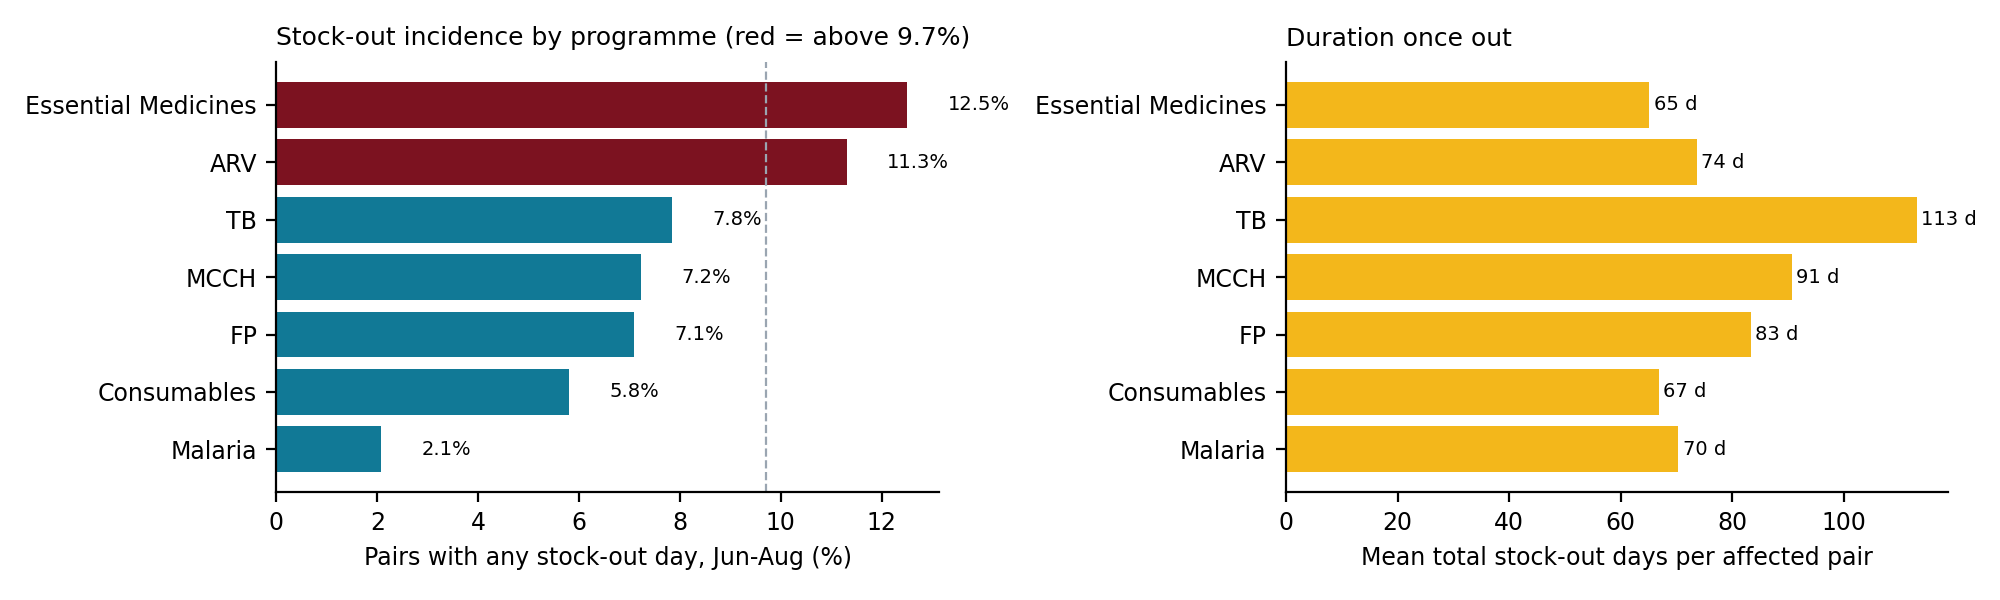
\includegraphics[width=0.96\linewidth]{d4_stockouts.png}\caption{Stock-out incidence and mean duration by programme.}\end{figure}
{\footnotesize\setlength{\tabcolsep}{3pt}\renewcommand{\arraystretch}{1.15}
\begin{longtable}{>{\raggedright\arraybackslash}p{0.316\linewidth}>{\raggedright\arraybackslash}p{0.152\linewidth}>{\raggedright\arraybackslash}p{0.177\linewidth}>{\raggedright\arraybackslash}p{0.164\linewidth}>{\raggedright\arraybackslash}p{0.152\linewidth}}
\caption{Stock-out incidence by level of care and management type}\\
\rowcolor{navy}\textbf{\color{white}Group} & \textbf{\color{white}Facilities} & \textbf{\color{white}Observations} & \textbf{\color{white}Numerator} & \textbf{\color{white}RATE} \\
\endfirsthead
\rowcolor{navy}\textbf{\color{white}Group} & \textbf{\color{white}Facilities} & \textbf{\color{white}Observations} & \textbf{\color{white}Numerator} & \textbf{\color{white}RATE} \\
\endhead
Health post & 25 & 555 & 45 & 8.1\% \\
\rowcolor{band}Health centre & 205 & 7,517 & 772 & 10.3\% \\
District hospital & 24 & 1,025 & 57 & 5.6\% \\
\rowcolor{band}Level 2 teaching hospital & 10 & 445 & 47 & 10.6\% \\
National referral hospital & 2 & 86 & 12 & 14.0\% \\
\end{longtable}}
\begin{figure}[H]\centering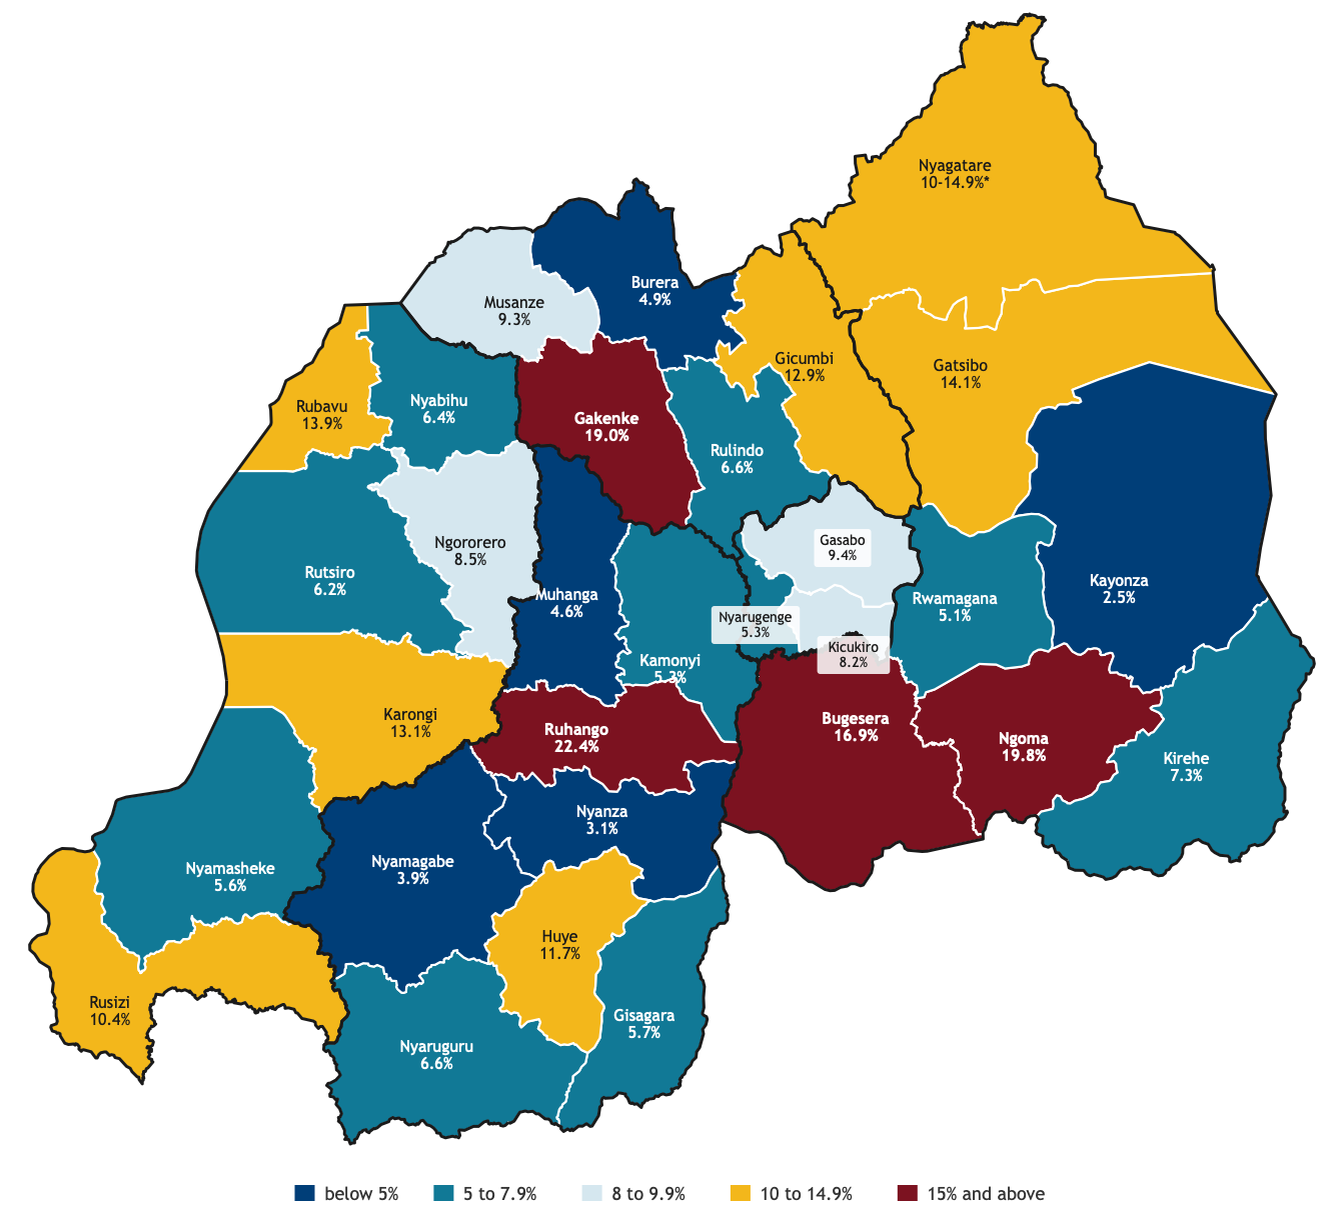
\includegraphics[width=0.66\linewidth]{map_so.png}\caption{Stock-out incidence by district.}\end{figure}
{\footnotesize\setlength{\tabcolsep}{3pt}\renewcommand{\arraystretch}{1.15}
\begin{longtable}{>{\raggedright\arraybackslash}p{0.349\linewidth}>{\raggedright\arraybackslash}p{0.164\linewidth}>{\raggedright\arraybackslash}p{0.109\linewidth}>{\raggedright\arraybackslash}p{0.109\linewidth}>{\raggedright\arraybackslash}p{0.109\linewidth}>{\raggedright\arraybackslash}p{0.120\linewidth}}
\caption{Medicines with the heaviest stock-out burden (30 or more managed pairs)}\\
\rowcolor{navy}\textbf{\color{white}Medicine} & \textbf{\color{white}Programme} & \textbf{\color{white}Managed pairs} & \textbf{\color{white}Pairs ever out} & \textbf{\color{white}INCIDENCE} & \textbf{\color{white}Average days out} \\
\endfirsthead
\rowcolor{navy}\textbf{\color{white}Medicine} & \textbf{\color{white}Programme} & \textbf{\color{white}Managed pairs} & \textbf{\color{white}Pairs ever out} & \textbf{\color{white}INCIDENCE} & \textbf{\color{white}Average days out} \\
\endhead
AMLODIPIN/LOSART/HTZ 5MG/50MG/12.5MG TAB & Essential Medicines & 2 & 1 & 50.0\% & 178 \\
\rowcolor{band}Vitamin B1 tablet(Thiamine) 50mg & Essential Medicines & 147 & 68 & 46.3\% & 112 \\
THIAMINE 100MG (VIT B1)TABLET & Essential Medicines & 155 & 60 & 38.7\% & 93.7 \\
\rowcolor{band}INSULIN HUM 100UI/ML 10MLS FAST SC INJ & Essential Medicines & 98 & 34 & 34.7\% & 50.1 \\
HYDROCHLOROTHIAZIDE 50MG TAB & Essential Medicines & 8 & 2 & 25.0\% & 117 \\
\rowcolor{band}HIV-1/2  Determine HIV Early Detect  100 Tests & ARV & 250 & 57 & 22.8\% & 59.4 \\
BECLOMETHASONE INHALATION SOLUTION 250MCG/DOSE & Essential Medicines & 153 & 34 & 22.2\% & 96.1 \\
\rowcolor{band}RIFAMP 75+ISONIAZID 50+ PYRAZINAMID150/84 & TB & 124 & 26 & 21.0\% & 128.6 \\
Diclofenac Suppository & Essential Medicines & 195 & 38 & 19.5\% & 83.9 \\
\rowcolor{band}Polyglactin 910 1 coated 1/2 circle round body 37mm L:75cm & Consumables & 63 & 12 & 19.0\% & 107.1 \\
Amlodipine 5mg & Essential Medicines & 191 & 34 & 17.8\% & 48.3 \\
\rowcolor{band}Abacavir/Lamivudine/Dolutegravir 60/30/5mg 180 Tabs & ARV & 188 & 32 & 17.0\% & 95.7 \\
Amlodipine 10mg & Essential Medicines & 114 & 19 & 16.7\% & 71.7 \\
\rowcolor{band}CIRPOFLOXACIN 500MG TAB & Essential Medicines & 247 & 37 & 15.0\% & 58 \\
\end{longtable}}
Stock-outs are uncommon for programme products but long once they occur (65-113 days on average). Thiamine (both strengths), insulin, HIV test kits, beclomethasone and paediatric RHZ carry the heaviest burden. 219 of 266 facilities had at least one stock-out in the period.

\section{Inferential findings}
\subsection{Factors associated with stock-outs}
{\footnotesize\setlength{\tabcolsep}{3pt}\renewcommand{\arraystretch}{1.15}
\begin{longtable}{>{\raggedright\arraybackslash}p{0.565\linewidth}>{\raggedright\arraybackslash}p{0.248\linewidth}>{\raggedright\arraybackslash}p{0.147\linewidth}}
\caption{Model 2: adjusted odds ratios for any stock-out day, June-August}\\
\rowcolor{navy}\textbf{\color{white}Factor} & \textbf{\color{white}Adjusted OR (95\% CI)} & \textbf{\color{white}p} \\
\endfirsthead
\rowcolor{navy}\textbf{\color{white}Factor} & \textbf{\color{white}Adjusted OR (95\% CI)} & \textbf{\color{white}p} \\
\endhead
Level: District hospital (ref. Health centre) & 0.64 (0.39-1.05) & 0.080 \\
\rowcolor{band}Level: Health post (ref. Health centre) & 0.53 (0.28-1.02) & 0.059 \\
Level: Referral / teaching (ref. Health centre) & 1.43 (0.78-2.61) & 0.251 \\
\rowcolor{band}Management: Faith-based (ref. Government) & 0.76 (0.55-1.04) & 0.090 \\
Management: PPP (ref. Government) & 1.28 (0.80-2.06) & 0.304 \\
\rowcolor{band}Province: East (ref. Kigali City) & 1.69 (1.06-2.68) & 0.027 \\
Province: North (ref. Kigali City) & 1.54 (0.99-2.39) & 0.056 \\
\rowcolor{band}Province: South (ref. Kigali City) & 1.20 (0.71-2.02) & 0.492 \\
Province: West (ref. Kigali City) & 1.52 (0.97-2.38) & 0.069 \\
\rowcolor{band}Programme: ARV (ref. Essential Medicines) & 0.49 (0.38-0.62) & $<$0.001 \\
Programme: Consumables (ref. Essential Medicines) & 0.38 (0.29-0.50) & $<$0.001 \\
\rowcolor{band}Programme: FP (ref. Essential Medicines) & 0.26 (0.19-0.35) & $<$0.001 \\
Programme: MCCH (ref. Essential Medicines) & 0.25 (0.19-0.34) & $<$0.001 \\
\rowcolor{band}Programme: Malaria (ref. Essential Medicines) & 0.06 (0.04-0.11) & $<$0.001 \\
Programme: TB (ref. Essential Medicines) & 0.36 (0.26-0.50) & $<$0.001 \\
\rowcolor{band}Setting: urban (ref. rural) & 1.05 (0.74-1.50) & 0.766 \\
log(AMC + 1) & 0.79 (0.75-0.82) & $<$0.001 \\
\rowcolor{band}Erratic consumption (CV $\geq$ 50\%) & 1.33 (1.13-1.55) & $<$0.001 \\
Facility fill rate (per +10 points) & 0.98 (0.86-1.11) & 0.713 \\
\rowcolor{band}Facility record accuracy (per +10 points) & 1.01 (0.97-1.04) & 0.730 \\
\multicolumn{3}{p{0.96\linewidth}}{\scriptsize\itshape\color{gray} Outcome: any stock-out day June-August. n = 9,590 pairs.}\\
\end{longtable}}
\begin{figure}[H]\centering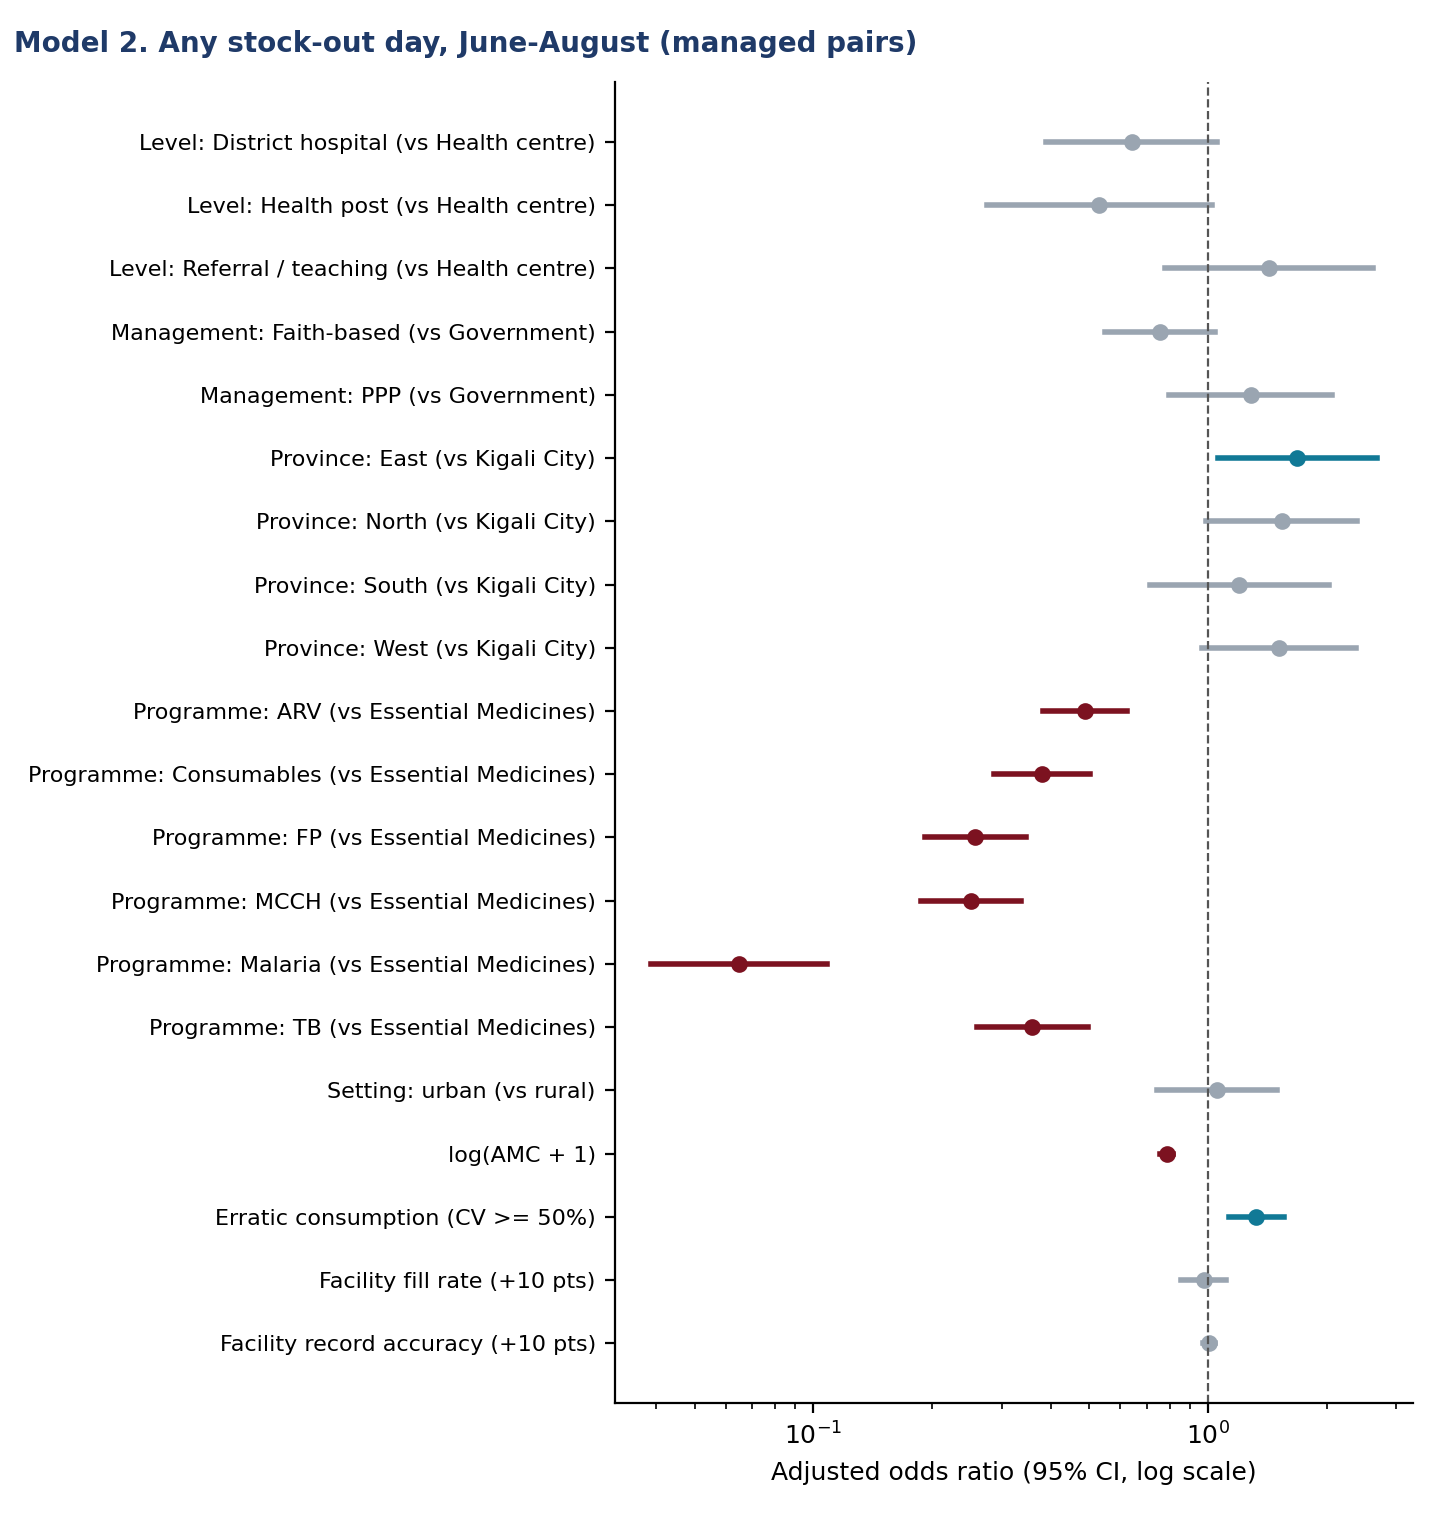
\includegraphics[width=0.78\linewidth]{fig_forest_stockout.png}\caption{Adjusted odds ratios for stock-out incidence.}\end{figure}
\textbf{Interpretation.} Every vertical programme has far lower odds of a stock-out than essential medicines (OR 0.06 for malaria to 0.49 for ARV). This reflects separate, programme-managed pipelines with push distribution and larger buffer stocks, which is also why these programmes are the most overstocked. Higher-volume medicines are less often out (OR 0.79 (0.75-0.82) per unit log AMC), and medicines with erratic month-to-month consumption more often (OR 1.33 (1.13-1.55)): an average-based order quantity fails exactly where demand is irregular. Eastern facilities have higher odds than Kigali City (OR 1.69 (1.06-2.68)).

\subsection{Does order fulfilment drive stock-outs?}
{\footnotesize\setlength{\tabcolsep}{3pt}\renewcommand{\arraystretch}{1.15}
\begin{longtable}{>{\raggedright\arraybackslash}p{0.395\linewidth}>{\raggedright\arraybackslash}p{0.226\linewidth}>{\raggedright\arraybackslash}p{0.339\linewidth}}
\caption{Stock-out next month by this month's order outcome}\\
\rowcolor{navy}\textbf{\color{white}Order outcome this month} & \textbf{\color{white}Pair-months} & \textbf{\color{white}Stocked out next month} \\
\endfirsthead
\rowcolor{navy}\textbf{\color{white}Order outcome this month} & \textbf{\color{white}Pair-months} & \textbf{\color{white}Stocked out next month} \\
\endhead
Delivered in full & 6,848 & 2.9\% \\
\rowcolor{band}No request & 11,669 & 7.9\% \\
Partly delivered & 300 & 4.3\% \\
\rowcolor{band}Requested, nothing delivered & 363 & 36.9\% \\
\end{longtable}}
{\footnotesize\setlength{\tabcolsep}{3pt}\renewcommand{\arraystretch}{1.15}
\begin{longtable}{>{\raggedright\arraybackslash}p{0.565\linewidth}>{\raggedright\arraybackslash}p{0.248\linewidth}>{\raggedright\arraybackslash}p{0.147\linewidth}}
\caption{Model 4: adjusted odds ratios for a stock-out next month}\\
\rowcolor{navy}\textbf{\color{white}Factor} & \textbf{\color{white}Adjusted OR (95\% CI)} & \textbf{\color{white}p} \\
\endfirsthead
\rowcolor{navy}\textbf{\color{white}Factor} & \textbf{\color{white}Adjusted OR (95\% CI)} & \textbf{\color{white}p} \\
\endhead
Order outcome this month: No request (ref. Delivered in full) & 2.64 (1.94-3.61) & $<$0.001 \\
\rowcolor{band}Order outcome this month: Partly delivered (ref. Delivered in full) & 0.54 (0.23-1.28) & 0.165 \\
Order outcome this month: Requested, nothing delivered (ref. Delivered in full) & 7.62 (4.57-12.70) & $<$0.001 \\
\rowcolor{band}Month: August & 0.93 (0.77-1.14) & 0.491 \\
Level: District hospital (ref. Health centre) & 0.69 (0.47-1.00) & 0.049 \\
\rowcolor{band}Level: Health post (ref. Health centre) & 0.73 (0.47-1.12) & 0.151 \\
Level: Referral / teaching (ref. Health centre) & 1.67 (1.06-2.63) & 0.027 \\
\rowcolor{band}Programme: ARV (ref. Essential Medicines) & 0.68 (0.50-0.92) & 0.013 \\
Programme: Consumables (ref. Essential Medicines) & 0.59 (0.44-0.79) & $<$0.001 \\
\rowcolor{band}Programme: FP (ref. Essential Medicines) & 0.50 (0.38-0.64) & $<$0.001 \\
Programme: MCCH (ref. Essential Medicines) & 0.46 (0.34-0.61) & $<$0.001 \\
\rowcolor{band}Programme: Malaria (ref. Essential Medicines) & 0.12 (0.08-0.17) & $<$0.001 \\
Programme: TB (ref. Essential Medicines) & 0.46 (0.34-0.62) & $<$0.001 \\
\rowcolor{band}Stocked out this month & 117.39 (91.96-149.85) & $<$0.001 \\
log(AMC + 1) & 0.89 (0.86-0.93) & $<$0.001 \\
\multicolumn{3}{p{0.96\linewidth}}{\scriptsize\itshape\color{gray} Outcome: any stock-out day in month t+1. n = 19,180 pair-months.}\\
\end{longtable}}
\begin{figure}[H]\centering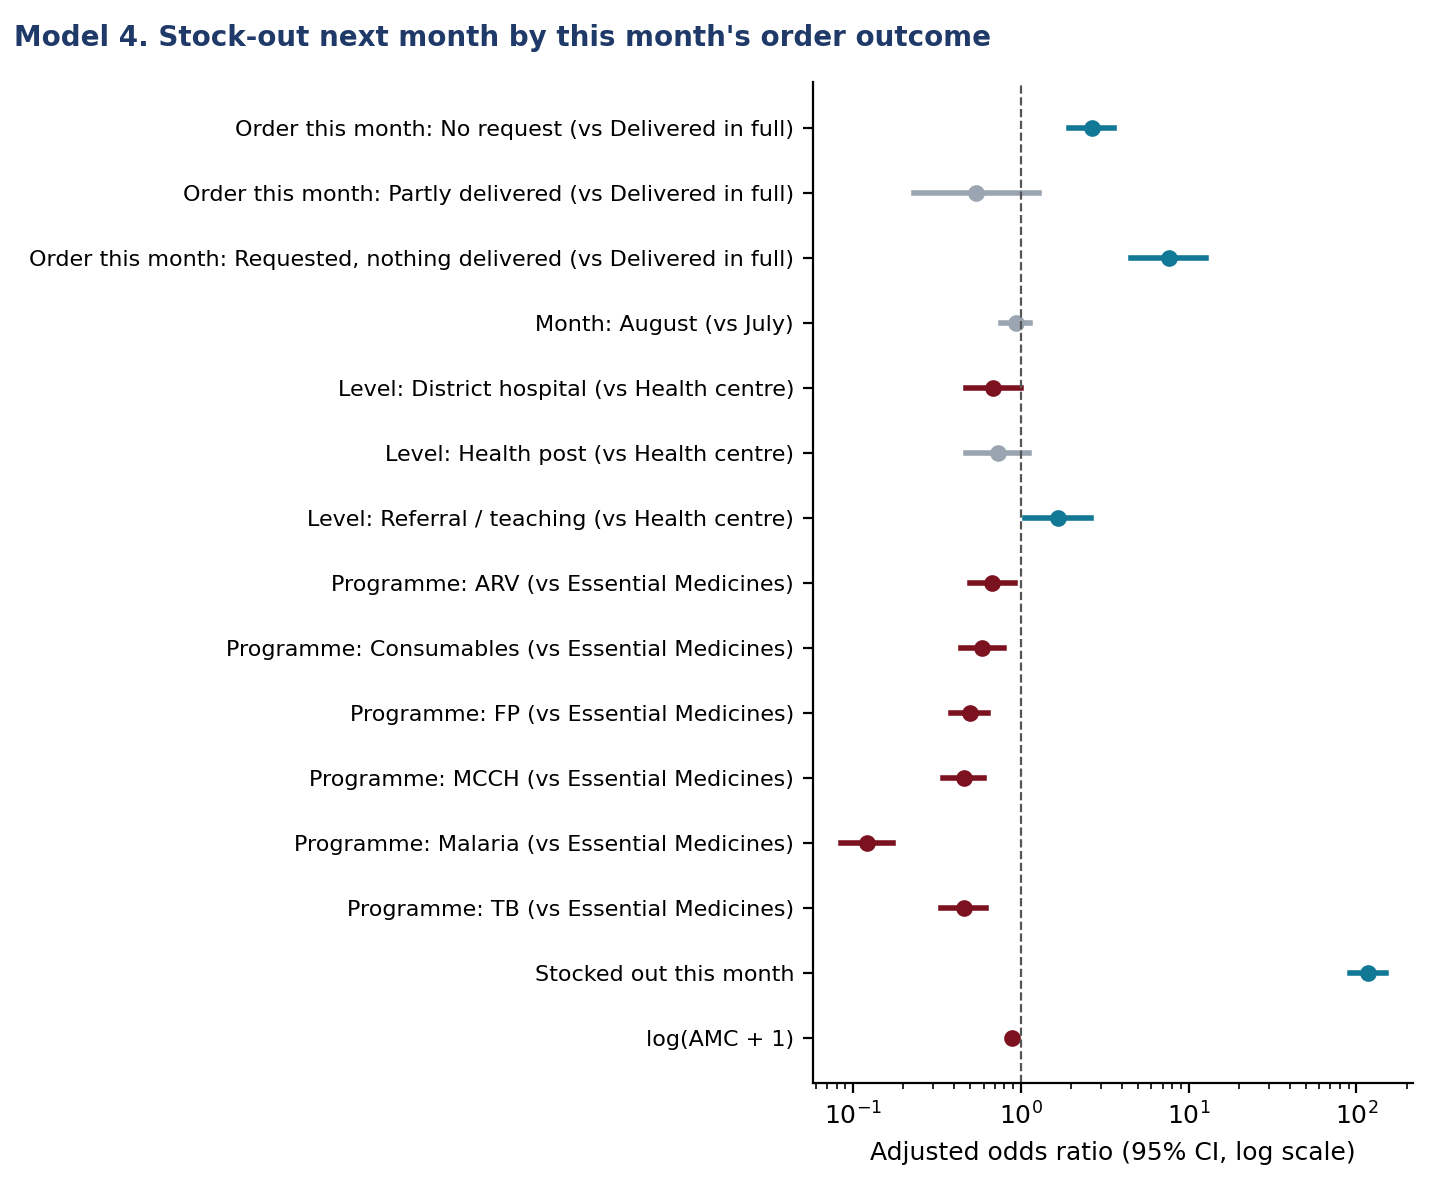
\includegraphics[width=0.78\linewidth]{fig_forest_lag.png}\caption{Next-month stock-out by this month's order outcome.}\end{figure}
\textbf{Interpretation.} This is the clearest causal signal in the data, because the exposure precedes the outcome. When a facility requested a medicine and received nothing, 36.9\% of those pairs were out the next month, and the adjusted odds were 7.6 times those after a full delivery, even after accounting for whether the medicine was already out. Partial deliveries carried no excess risk, so the problem is orders that go entirely unfilled, not quantities trimmed. Not requesting at all also raised the odds (OR 2.64 (1.94-3.61)), pointing to missed or late orders at the facility. Being out this month was by far the strongest predictor (OR 117): once a stock-out starts it tends to last. Together these support two actions: RMS should flag and expedite nil-filled orders, and facilities should not skip a requisition cycle.

\chapter{Prescription fulfilment (objective 4)}
\section{Descriptive findings}
5,934 of 6,006 prescriptions (98.8\%) were fully served; 58 were partly served (1.0\%) and 14 had nothing available (0.2\%). 107 of 14,059 prescribed items (0.8\%) were unserved. National referral hospitals stand out: 23 of 70 prescriptions (32.9\%) and 15.6\% of items were unserved.

{\footnotesize\setlength{\tabcolsep}{3pt}\renewcommand{\arraystretch}{1.15}
\begin{longtable}{>{\raggedright\arraybackslash}p{0.227\linewidth}>{\raggedright\arraybackslash}p{0.097\linewidth}>{\raggedright\arraybackslash}p{0.119\linewidth}>{\raggedright\arraybackslash}p{0.129\linewidth}>{\raggedright\arraybackslash}p{0.086\linewidth}>{\raggedright\arraybackslash}p{0.097\linewidth}>{\raggedright\arraybackslash}p{0.108\linewidth}>{\raggedright\arraybackslash}p{0.097\linewidth}}
\caption{Prescription fulfilment by level of care}\\
\rowcolor{navy}\textbf{\color{white}Level of care} & \textbf{\color{white}Facilities} & \textbf{\color{white}Prescriptions} & \textbf{\color{white}Prescriptions not fully served} & \textbf{\color{white}\%} & \textbf{\color{white}Items} & \textbf{\color{white}Unserved items} & \textbf{\color{white}Unserved \%} \\
\endfirsthead
\rowcolor{navy}\textbf{\color{white}Level of care} & \textbf{\color{white}Facilities} & \textbf{\color{white}Prescriptions} & \textbf{\color{white}Prescriptions not fully served} & \textbf{\color{white}\%} & \textbf{\color{white}Items} & \textbf{\color{white}Unserved items} & \textbf{\color{white}Unserved \%} \\
\endhead
Health post & 23 & 495 & 0 & 0.0\% & 1,090 & 0 & 0.0\% \\
\rowcolor{band}Health centre & 207 & 4,384 & 37 & 0.8\% & 10,064 & 46 & 0.5\% \\
District hospital & 24 & 739 & 10 & 1.4\% & 1,860 & 18 & 1.0\% \\
\rowcolor{band}Level 2 teaching hospital & 10 & 318 & 2 & 0.6\% & 782 & 2 & 0.3\% \\
National referral hospital & 2 & 70 & 23 & 32.9\% & 263 & 41 & 15.6\% \\
\end{longtable}}
{\footnotesize\setlength{\tabcolsep}{3pt}\renewcommand{\arraystretch}{1.15}
\begin{longtable}{>{\raggedright\arraybackslash}p{0.492\linewidth}>{\raggedright\arraybackslash}p{0.160\linewidth}>{\raggedright\arraybackslash}p{0.160\linewidth}>{\raggedright\arraybackslash}p{0.148\linewidth}}
\caption{Unserved items by drug class: the most affected}\\
\rowcolor{navy}\textbf{\color{white}Group} & \textbf{\color{white}Observations} & \textbf{\color{white}Numerator} & \textbf{\color{white}RATE} \\
\endfirsthead
\rowcolor{navy}\textbf{\color{white}Group} & \textbf{\color{white}Observations} & \textbf{\color{white}Numerator} & \textbf{\color{white}RATE} \\
\endhead
23.5 Insulins and other medicines used for diabetes & 170 & 19 & 11.2\% \\
\rowcolor{band}26. MEDICINES ACTING ON THE RESPIRATORY TRACT & 69 & 5 & 7.2\% \\
21.1 Anti-anaemia medicines & 75 & 3 & 4.0\% \\
\rowcolor{band}15.2 Antiemetic medicines & 34 & 1 & 2.9\% \\
12.1.2 Antibacterials and Antiparasitics & 40 & 1 & 2.5\% \\
\rowcolor{band}8.2.1 Medicines used in depressive disorders & 46 & 1 & 2.2\% \\
12.1.3 Antifungal medicines & 132 & 2 & 1.5\% \\
\rowcolor{band}5.2 Specific & 146 & 2 & 1.4\% \\
\end{longtable}}
{\footnotesize\setlength{\tabcolsep}{3pt}\renewcommand{\arraystretch}{1.15}
\begin{longtable}{>{\raggedright\arraybackslash}p{0.468\linewidth}>{\raggedright\arraybackslash}p{0.117\linewidth}>{\raggedright\arraybackslash}p{0.140\linewidth}>{\raggedright\arraybackslash}p{0.117\linewidth}>{\raggedright\arraybackslash}p{0.117\linewidth}}
\caption{Most frequently unserved medicines}\\
\rowcolor{navy}\textbf{\color{white}Medicine} & \textbf{\color{white}Unserved} & \textbf{\color{white}Times prescribed} & \textbf{\color{white}Unserved \%} & \textbf{\color{white}Facilities} \\
\endfirsthead
\rowcolor{navy}\textbf{\color{white}Medicine} & \textbf{\color{white}Unserved} & \textbf{\color{white}Times prescribed} & \textbf{\color{white}Unserved \%} & \textbf{\color{white}Facilities} \\
\endhead
Long-acting insulins - Inj.100 IU/ml & 7 & 14 & 50.0\% & 3 \\
\rowcolor{band}Ciprofloxacin - Tab. 500mg & 6 & 258 & 2.3\% & 2 \\
Amlodipine / Losartan/ Hydrochlorothiazide - Tab. 5mg/50mg/12.5mg & 4 & 7 & 57.1\% & 1 \\
\rowcolor{band}Chlorpheniramine +Ammonium Chloride +Sodium citrate +Menthol - Syrup: 2.2mg /110mg/40mg/1.1mg & 3 & 3 & 100.0\% & 1 \\
Intermediate- acting insulins - Inj. 100 IU/ml & 3 & 3 & 100.0\% & 1 \\
\rowcolor{band}Nebilong 5mg & 3 & 3 & 100.0\% & 1 \\
Rapid acting insulins inj 100 iu ml & 3 & 13 & 23.1\% & 2 \\
\rowcolor{band}Metformin - Tab. 500 mg & 3 & 60 & 5.0\% & 2 \\
Thiamine - Tab. 50 mg/ 100mg & 3 & 289 & 1.0\% & 3 \\
\rowcolor{band}Ibuprofen - Tab. 400 mg & 3 & 1,034 & 0.3\% & 2 \\
\end{longtable}}
Unserved prescribing clusters in insulins and diabetes medicines and in respiratory medicines. Because prescribers tend to write what the pharmacy holds, these rates understate true unmet need; the stock-based indicators are the better guide to availability.

\section{Inferential findings}
\subsection{Prescribing quality and unserved prescriptions}
{\footnotesize\setlength{\tabcolsep}{3pt}\renewcommand{\arraystretch}{1.15}
\begin{longtable}{>{\raggedright\arraybackslash}p{0.294\linewidth}>{\raggedright\arraybackslash}p{0.237\linewidth}>{\raggedright\arraybackslash}p{0.169\linewidth}>{\raggedright\arraybackslash}p{0.260\linewidth}}
\caption{WHO/INRUD prescribing indicators}\\
\rowcolor{navy}\textbf{\color{white}WHO indicator} & \textbf{\color{white}Estimate (95\% CI)} & \textbf{\color{white}WHO reference} & \textbf{\color{white}Africa median [Ofori-Asenso 2016]} \\
\endfirsthead
\rowcolor{navy}\textbf{\color{white}WHO indicator} & \textbf{\color{white}Estimate (95\% CI)} & \textbf{\color{white}WHO reference} & \textbf{\color{white}Africa median [Ofori-Asenso 2016]} \\
\endhead
Medicines per encounter & 2.25 (2.14-2.36) & $<$ 2 (1.6-1.8) & 3.1 \\
\rowcolor{band}Generic (INN) prescribing & 97.2\% (95.3-99.1) & 100\% & 68.0\% \\
Encounters with an antibiotic & 49.5\% (44.9-54.2) & $<$ 30\% & 46.8\% \\
\rowcolor{band}Encounters with an injection & 8.8\% (6.2-11.5) & $<$ 20\% & 25.0\% \\
Medicines from the EML & 95.4\% (90.3-100.0) & 100\% & 88.0\% \\
\multicolumn{4}{p{0.96\linewidth}}{\scriptsize\itshape\color{gray} Weighted by level; facility-clustered 95\% CI.}\\
\end{longtable}}
{\footnotesize\setlength{\tabcolsep}{3pt}\renewcommand{\arraystretch}{1.15}
\begin{longtable}{>{\raggedright\arraybackslash}p{0.294\linewidth}>{\raggedright\arraybackslash}p{0.158\linewidth}>{\raggedright\arraybackslash}p{0.181\linewidth}>{\raggedright\arraybackslash}p{0.164\linewidth}>{\raggedright\arraybackslash}p{0.164\linewidth}}
\caption{Prescribing indicators by level of care}\\
\rowcolor{navy}\textbf{\color{white}Level} & \textbf{\color{white}Prescriptions} & \textbf{\color{white}Medicines / encounter} & \textbf{\color{white}\% antibiotic} & \textbf{\color{white}\% injection} \\
\endfirsthead
\rowcolor{navy}\textbf{\color{white}Level} & \textbf{\color{white}Prescriptions} & \textbf{\color{white}Medicines / encounter} & \textbf{\color{white}\% antibiotic} & \textbf{\color{white}\% injection} \\
\endhead
District hospital & 739 & 2.52 & 36.9 & 30.0 \\
\rowcolor{band}Health centre & 4384 & 2.30 & 50.5 & 9.2 \\
Health post & 495 & 2.20 & 50.1 & 7.3 \\
\rowcolor{band}Level 2 teaching hospital & 318 & 2.46 & 34.3 & 31.4 \\
National referral hospital & 70 & 3.76 & 15.7 & 25.7 \\
\end{longtable}}
\begin{figure}[H]\centering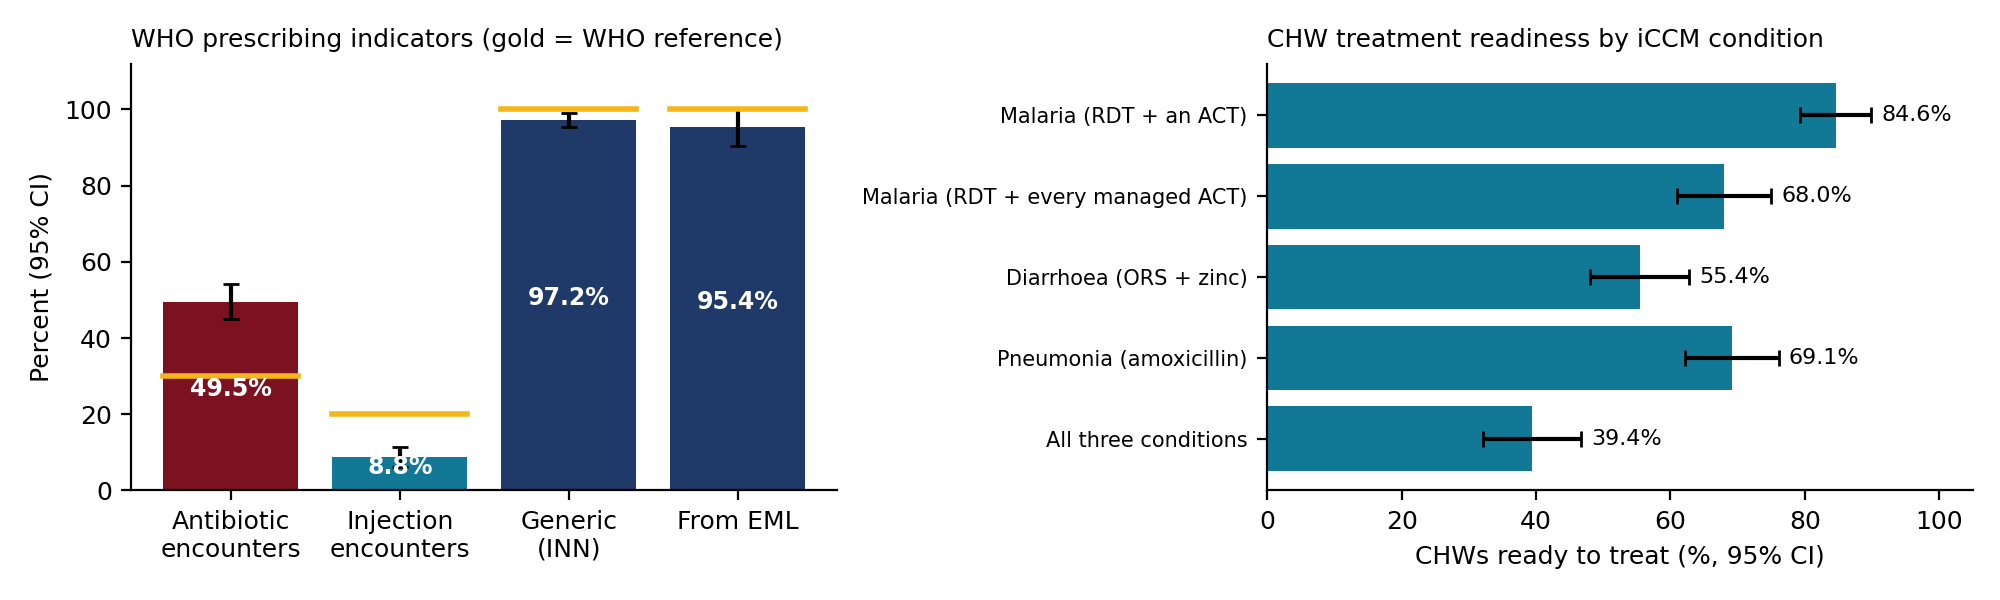
\includegraphics[width=0.96\linewidth]{fig_who_iccm.png}\caption{WHO prescribing indicators (left) and CHW readiness by iCCM condition (right).}\end{figure}
{\footnotesize\setlength{\tabcolsep}{3pt}\renewcommand{\arraystretch}{1.15}
\begin{longtable}{>{\raggedright\arraybackslash}p{0.452\linewidth}>{\raggedright\arraybackslash}p{0.254\linewidth}>{\raggedright\arraybackslash}p{0.254\linewidth}}
\caption{Models 5 and 6: unserved prescriptions and antibiotic prescribing}\\
\rowcolor{navy}\textbf{\color{white}Factor} & \textbf{\color{white}Unserved: OR (95\% CI)} & \textbf{\color{white}Antibiotic: OR (95\% CI)} \\
\endfirsthead
\rowcolor{navy}\textbf{\color{white}Factor} & \textbf{\color{white}Unserved: OR (95\% CI)} & \textbf{\color{white}Antibiotic: OR (95\% CI)} \\
\endhead
Prescriber: General practitioner (ref. Nurse) & 0.98 (0.20-4.88) & 2.18 (1.27-3.73) \\
\rowcolor{band}Prescriber: Other (ref. Nurse) & 3.23 (0.97-10.74) & 1.63 (0.99-2.67) \\
Prescriber: Specialist (ref. Nurse) & 10.16 (1.33-77.34) & 0.80 (0.28-2.31) \\
\rowcolor{band}Level: District hospital (ref. Primary care (HC/HP)) & 1.10 (0.26-4.67) & 0.25 (0.15-0.41) \\
Level: Referral / teaching (ref. Primary care (HC/HP)) & 2.14 (0.38-11.92) & 0.18 (0.10-0.34) \\
\rowcolor{band}Medicines on the prescription (per +1) & 1.34 (1.15-1.55) & 2.08 (1.88-2.31) \\
\multicolumn{3}{p{0.96\linewidth}}{\scriptsize\itshape\color{gray} Models 5 and 6. Outcomes: any unserved item; any antibiotic. Reference: nurse, primary care.}\\
\end{longtable}}
\textbf{Interpretation.} Prescribing in Rwanda compares well with the African median on generic names, EML adherence, polypharmacy and injections. Antibiotic use is the exception: 49.5\% of encounters, about the African median and well above the 30\% reference. It is concentrated in primary care (about half of health-centre and health-post encounters, against about a third in hospitals), and general practitioners prescribe antibiotics more often than nurses once the number of medicines is held constant (OR 2.18 (1.27-3.73)). This is a priority for antimicrobial stewardship. Unserved prescriptions are rare, but a specialist's prescription is far more likely to include an unavailable item (OR 10.16 (1.33-77.34)), as is a longer prescription (OR 1.34 (1.15-1.55) per medicine). This matches the referral-hospital gaps on the dashboard: specialist prescribing reaches beyond what the pharmacy stocks.

\chapter{Supply chain attribution (objective 5)}
For medicines unavailable at the facility, teams recorded whether the product was in stock at RMS Regional and RMS Central. Of 448 unavailable items with both answers, 384 (85.7\%) were in stock at one or both RMS levels: a distribution gap between RMS and the facility rather than a national shortage. Missing items were more often in stock at RMS Central than at RMS Regional, by 4 to 16 points depending on level.

{\footnotesize\setlength{\tabcolsep}{3pt}\renewcommand{\arraystretch}{1.15}
\begin{longtable}{>{\raggedright\arraybackslash}p{0.300\linewidth}>{\raggedright\arraybackslash}p{0.120\linewidth}>{\raggedright\arraybackslash}p{0.180\linewidth}>{\raggedright\arraybackslash}p{0.180\linewidth}>{\raggedright\arraybackslash}p{0.180\linewidth}}
\caption{Unavailable items in stock upstream, by level of care}\\
\rowcolor{navy}\textbf{\color{white}Level of care} & \textbf{\color{white}Items} & \textbf{\color{white}At RMS Central} & \textbf{\color{white}At RMS Regional} & \textbf{\color{white}Distribution gap} \\
\endfirsthead
\rowcolor{navy}\textbf{\color{white}Level of care} & \textbf{\color{white}Items} & \textbf{\color{white}At RMS Central} & \textbf{\color{white}At RMS Regional} & \textbf{\color{white}Distribution gap} \\
\endhead
Health post & 36 & 91.7\% & 80.6\% & 91.7\% \\
\rowcolor{band}Health centre & 367 & 84.2\% & 79.8\% & 85.8\% \\
District hospital & 19 & 94.7\% & 78.9\% & 94.7\% \\
\rowcolor{band}Level 2 teaching hospital & 22 & 72.7\% & 63.6\% & 72.7\% \\
National referral hospital & 4 & 50.0\% & 50.0\% & 50.0\% \\
\end{longtable}}
{\footnotesize\setlength{\tabcolsep}{3pt}\renewcommand{\arraystretch}{1.15}
\begin{longtable}{>{\raggedright\arraybackslash}p{0.338\linewidth}>{\raggedright\arraybackslash}p{0.162\linewidth}>{\raggedright\arraybackslash}p{0.230\linewidth}>{\raggedright\arraybackslash}p{0.230\linewidth}}
\caption{Distribution gap against nationwide stock-out, by programme (10 or more items)}\\
\rowcolor{navy}\textbf{\color{white}Programme} & \textbf{\color{white}Items} & \textbf{\color{white}Distribution gap} & \textbf{\color{white}Nationwide stock-out} \\
\endfirsthead
\rowcolor{navy}\textbf{\color{white}Programme} & \textbf{\color{white}Items} & \textbf{\color{white}Distribution gap} & \textbf{\color{white}Nationwide stock-out} \\
\endhead
ARV & 65 & 47.7\% & 52.3\% \\
\rowcolor{band}Consumables & 25 & 96.0\% & 4.0\% \\
Essential Medicines & 231 & 91.8\% & 8.2\% \\
\rowcolor{band}FP & 50 & 86.0\% & 14.0\% \\
MCCH & 26 & 96.2\% & 3.8\% \\
\rowcolor{band}TB & 48 & 95.8\% & 4.2\% \\
\end{longtable}}
{\footnotesize\setlength{\tabcolsep}{3pt}\renewcommand{\arraystretch}{1.15}
\begin{longtable}{>{\raggedright\arraybackslash}p{0.379\linewidth}>{\raggedright\arraybackslash}p{0.142\linewidth}>{\raggedright\arraybackslash}p{0.107\linewidth}>{\raggedright\arraybackslash}p{0.095\linewidth}>{\raggedright\arraybackslash}p{0.119\linewidth}>{\raggedright\arraybackslash}p{0.119\linewidth}}
\caption{Medicines with a nationwide stock-out (not at the facility and not at RMS Central)}\\
\rowcolor{navy}\textbf{\color{white}Medicine} & \textbf{\color{white}Programme} & \textbf{\color{white}Facilities reporting it} & \textbf{\color{white}Districts} & \textbf{\color{white}Facilities managing it} & \textbf{\color{white}SHARE OF MANAGING FACILITIES} \\
\endfirsthead
\rowcolor{navy}\textbf{\color{white}Medicine} & \textbf{\color{white}Programme} & \textbf{\color{white}Facilities reporting it} & \textbf{\color{white}Districts} & \textbf{\color{white}Facilities managing it} & \textbf{\color{white}SHARE OF MANAGING FACILITIES} \\
\endhead
HIV-1/2  Determine HIV Early Detect  100 Tests & ARV & 32 & 13 & 250 & 12.8\% \\
\rowcolor{band}INSULIN HUM 100UI/ML 10MLS FAST SC INJ & Essential Medicines & 9 & 7 & 98 & 9.2\% \\
Levonorgestrel 75mg/rod, 2rod Implant+Inserter/Jadelle & FP & 4 & 4 & 217 & 1.8\% \\
\rowcolor{band}Levonorgestrel/Ethinyl Estradiol 150/30 mcg + Fe 75 mg, 28 Tablets/Cycle/Microgynon & FP & 3 & 3 & 219 & 1.4\% \\
RIFAMP 75+ISONIAZID 50+ PYRAZINAMID150/84 & TB & 3 & 2 & 124 & 2.4\% \\
\rowcolor{band}THIAMINE 100MG (VIT B1)TABLET & Essential Medicines & 3 & 3 & 155 & 1.9\% \\
Atazanavir/Ritonavir 300/100mg 30 Tabs & ARV & 2 & 2 & 214 & 0.9\% \\
\rowcolor{band}VITAMIN C 500MG TABLET(Ascorbic Acid) & Essential Medicines & 2 & 2 & 259 & 0.8\% \\
Vitamin B1 tablet(Thiamine) 50mg & Essential Medicines & 2 & 2 & 147 & 1.4\% \\
\rowcolor{band}AMLODIPIN/LOSART/HTZ 5MG/50MG/12.5MG TAB & Essential Medicines & 1 & 1 & 2 & 50.0\% \\
AMOXICILLIN/CLAVUL.ACID(1000/200)MG INJ. & Essential Medicines & 1 & 1 & 2 & 50.0\% \\
\rowcolor{band}BECLOMETHASONE INHALATION SOLUTION 250MCG/DOSE & Essential Medicines & 1 & 1 & 153 & 0.7\% \\
CIRPOFLOXACIN 500MG TAB & Essential Medicines & 1 & 1 & 247 & 0.4\% \\
\rowcolor{band}Chromic Catgut Dec 3.5 (2/0) PR 1/2 C & Consumables & 1 & 1 & 219 & 0.5\% \\
Copper-bearing intrauterine devices (IUD) & FP & 1 & 1 & 188 & 0.5\% \\
\rowcolor{band}METRONIDAZOLE 250 TAB & Essential Medicines & 1 & 1 & 262 & 0.4\% \\
MgSO4 (50\% injectable) & MCCH & 1 & 1 & 240 & 0.4\% \\
\end{longtable}}
ARV products are the exception to the distribution pattern: about half of ARV gaps were also out at RMS, a national supply problem driven by HIV Determine test kits (32 facilities in 13 districts). For prescriptions, RMS status was often unknown: 41 of 107 unserved lines had ''don't know'' for both stores, a gap in the attribution evidence.

\chapter{Requisition and order fulfilment (objective 6)}
Across June-August, facilities requested 38.1 million units and received 35.4 million: a quantity fill rate of 93.1\%, steady across months (92.6\% in June, 92.0\% in July, 94.7\% in August).

\begin{figure}[H]\centering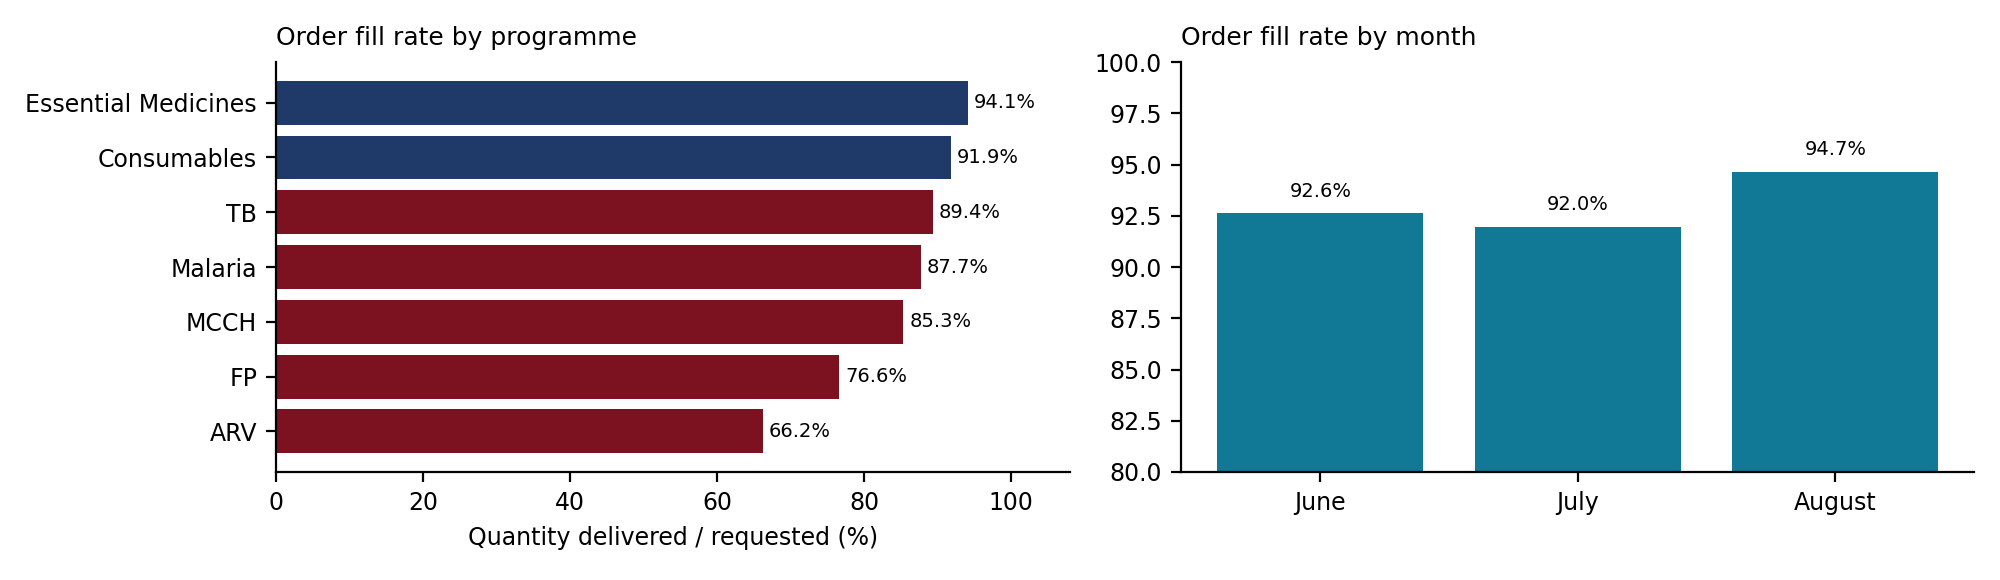
\includegraphics[width=0.96\linewidth]{d5_fill.png}\caption{Quantity fill rate by programme and by month.}\end{figure}
{\footnotesize\setlength{\tabcolsep}{3pt}\renewcommand{\arraystretch}{1.15}
\begin{longtable}{>{\raggedright\arraybackslash}p{0.312\linewidth}>{\raggedright\arraybackslash}p{0.125\linewidth}>{\raggedright\arraybackslash}p{0.187\linewidth}>{\raggedright\arraybackslash}p{0.187\linewidth}>{\raggedright\arraybackslash}p{0.150\linewidth}}
\caption{Quantity fill rate by level of care}\\
\rowcolor{navy}\textbf{\color{white}Level of care} & \textbf{\color{white}Facilities} & \textbf{\color{white}Requested} & \textbf{\color{white}Received} & \textbf{\color{white}FILL RATE} \\
\endfirsthead
\rowcolor{navy}\textbf{\color{white}Level of care} & \textbf{\color{white}Facilities} & \textbf{\color{white}Requested} & \textbf{\color{white}Received} & \textbf{\color{white}FILL RATE} \\
\endhead
Health post & 25 & 966,236 & 898,905 & 93.0\% \\
\rowcolor{band}Health centre & 205 & 20,595,340 & 19,336,023 & 93.9\% \\
District hospital & 24 & 8,271,795 & 7,849,296 & 94.9\% \\
\rowcolor{band}Level 2 teaching hospital & 10 & 6,461,457 & 5,978,328 & 92.5\% \\
National referral hospital & 2 & 1,761,464 & 1,366,116 & 77.6\% \\
\end{longtable}}
{\footnotesize\setlength{\tabcolsep}{3pt}\renewcommand{\arraystretch}{1.15}
\begin{longtable}{>{\raggedright\arraybackslash}p{0.294\linewidth}>{\raggedright\arraybackslash}p{0.128\linewidth}>{\raggedright\arraybackslash}p{0.192\linewidth}>{\raggedright\arraybackslash}p{0.192\linewidth}>{\raggedright\arraybackslash}p{0.154\linewidth}}
\caption{Quantity fill rate by programme}\\
\rowcolor{navy}\textbf{\color{white}Group} & \textbf{\color{white}Facilities} & \textbf{\color{white}Requested} & \textbf{\color{white}Delivered} & \textbf{\color{white}FILL RATE} \\
\endfirsthead
\rowcolor{navy}\textbf{\color{white}Group} & \textbf{\color{white}Facilities} & \textbf{\color{white}Requested} & \textbf{\color{white}Delivered} & \textbf{\color{white}FILL RATE} \\
\endhead
ARV & 252 & 430,799 & 285,242 & 66.2\% \\
\rowcolor{band}Consumables & 266 & 8,340,527 & 7,661,392 & 91.9\% \\
Essential Medicines & 266 & 28,248,612 & 26,592,230 & 94.1\% \\
\rowcolor{band}FP & 221 & 213,321 & 163,446 & 76.6\% \\
MCCH & 253 & 151,911 & 129,653 & 85.3\% \\
\rowcolor{band}Malaria & 265 & 202,635 & 177,810 & 87.7\% \\
TB & 240 & 468,437 & 418,845 & 89.4\% \\
\end{longtable}}
{\footnotesize\setlength{\tabcolsep}{3pt}\renewcommand{\arraystretch}{1.15}
\begin{longtable}{>{\raggedright\arraybackslash}p{0.360\linewidth}>{\raggedright\arraybackslash}p{0.131\linewidth}>{\raggedright\arraybackslash}p{0.131\linewidth}>{\raggedright\arraybackslash}p{0.131\linewidth}>{\raggedright\arraybackslash}p{0.098\linewidth}>{\raggedright\arraybackslash}p{0.109\linewidth}}
\caption{The most under-supplied medicines}\\
\rowcolor{navy}\textbf{\color{white}Medicine} & \textbf{\color{white}Requested} & \textbf{\color{white}Received} & \textbf{\color{white}Shortfall} & \textbf{\color{white}FILL RATE} & \textbf{\color{white}Stocked out on visit day} \\
\endfirsthead
\rowcolor{navy}\textbf{\color{white}Medicine} & \textbf{\color{white}Requested} & \textbf{\color{white}Received} & \textbf{\color{white}Shortfall} & \textbf{\color{white}FILL RATE} & \textbf{\color{white}Stocked out on visit day} \\
\endhead
AMLODIPIN/LOSART/HTZ 5MG/50MG/12.5MG TAB & 309,880 & 3,000 & 306,880 & 1.0\% & 1 \\
\rowcolor{band}CEFAZOLIN 1G IM/IV INJ & 51,600 & 4,800 & 46,800 & 9.3\% & 0 \\
AMOXICILLIN/CLAVUL.ACID(1000/200)MG INJ. & 6,030 & 860 & 5,170 & 14.3\% & 1 \\
\rowcolor{band}HIV-1/2  Determine HIV Early Detect  100 Tests & 331,030 & 193,874 & 137,156 & 58.6\% & 55 \\
Vitamin B1 tablet(Thiamine) 50mg & 511,098 & 321,952 & 189,146 & 63.0\% & 38 \\
\rowcolor{band}Levonorgestrel/Ethinyl Estradiol 150/30 mcg + Fe 75 mg, 28 Tablets/Cycle/Microgynon & 82,126 & 53,117 & 29,009 & 64.7\% & 15 \\
ARTE 20MG+LUME 120MG (1X6) & 1,730 & 1,160 & 570 & 67.1\% & 0 \\
\rowcolor{band}THIAMINE 100MG (VIT B1)TABLET & 687,020 & 477,020 & 210,000 & 69.4\% & 31 \\
Dihydroartemisinin/Piperaquine (DHAP) 20/160 mg Disp Tablet & 13,800 & 9,660 & 4,140 & 70.0\% & 1 \\
\rowcolor{band}Levonorgestrel 75mg/rod, 2rod Implant+Inserter/Jadelle & 19,111 & 13,860 & 5,251 & 72.5\% & 18 \\
\end{longtable}}
ARV (66.2\%), family planning (76.6\%) and MCCH (85.3\%) are filled least, and national referral hospitals received 77.6\% of their requests, falling to 20\% in July and 35\% in August. Among unserved prescription items, only 31.8\% had been ordered that month, and three quarters of those orders were not supplied at all.

{\footnotesize\setlength{\tabcolsep}{3pt}\renewcommand{\arraystretch}{1.15}
\begin{longtable}{>{\raggedright\arraybackslash}p{0.519\linewidth}>{\raggedright\arraybackslash}p{0.156\linewidth}>{\raggedright\arraybackslash}p{0.156\linewidth}>{\raggedright\arraybackslash}p{0.130\linewidth}}
\caption{Requisition rate for unserved prescription items}\\
\rowcolor{navy}\textbf{\color{white}Metric} & \textbf{\color{white}Numerator} & \textbf{\color{white}Denominator} & \textbf{\color{white}Rate} \\
\endfirsthead
\rowcolor{navy}\textbf{\color{white}Metric} & \textbf{\color{white}Numerator} & \textbf{\color{white}Denominator} & \textbf{\color{white}Rate} \\
\endhead
Unserved items that had been ordered that month & 34 & 107 & 31.8\% \\
\rowcolor{band}Unserved items never ordered & 73 & 107 & 68.2\% \\
\end{longtable}}
{\footnotesize\setlength{\tabcolsep}{3pt}\renewcommand{\arraystretch}{1.15}
\begin{longtable}{>{\raggedright\arraybackslash}p{0.480\linewidth}>{\raggedright\arraybackslash}p{0.240\linewidth}>{\raggedright\arraybackslash}p{0.240\linewidth}}
\caption{Outcome of the order where one was placed (unserved items)}\\
\rowcolor{navy}\textbf{\color{white}Supply outcome} & \textbf{\color{white}Lines} & \textbf{\color{white}\% of ordered} \\
\endfirsthead
\rowcolor{navy}\textbf{\color{white}Supply outcome} & \textbf{\color{white}Lines} & \textbf{\color{white}\% of ordered} \\
\endhead
Not at all & 25 & 73.5\% \\
\rowcolor{band}Fully & 5 & 14.7\% \\
Partially & 4 & 11.8\% \\
\end{longtable}}
\chapter{Financial value (objective 7)}
Unserved prescription items were valued at official tariff prices: 834,418 RWF in total, heavily concentrated at national referral hospitals and in a few high-cost combination products. Separately, sales lost to stock-outs were estimated for each managed pair from its in-stock consumption and the days it was out: 847,646 units worth 45,756,324 RWF over June-August including the facility's 20\% margin.

{\footnotesize\setlength{\tabcolsep}{3pt}\renewcommand{\arraystretch}{1.15}
\begin{longtable}{>{\raggedright\arraybackslash}p{0.343\linewidth}>{\raggedright\arraybackslash}p{0.206\linewidth}>{\raggedright\arraybackslash}p{0.233\linewidth}>{\raggedright\arraybackslash}p{0.178\linewidth}}
\caption{Unserved value by level of care and province}\\
\rowcolor{navy}\textbf{\color{white}Group} & \textbf{\color{white}Unserved lines} & \textbf{\color{white}Value (RWF)} & \textbf{\color{white}\% of total} \\
\endfirsthead
\rowcolor{navy}\textbf{\color{white}Group} & \textbf{\color{white}Unserved lines} & \textbf{\color{white}Value (RWF)} & \textbf{\color{white}\% of total} \\
\endhead
Health centre & 46 & 76,164 & 9.1\% \\
\rowcolor{band}District hospital & 18 & 149,537 & 17.9\% \\
Level 2 teaching hospital & 2 & 0 & 0.0\% \\
\rowcolor{band}National referral hospital & 41 & 608,717 & 73.0\% \\
East & 11 & 14,877 & 1.8\% \\
\rowcolor{band}Kigali City & 61 & 666,767 & 79.9\% \\
North & 1 & 530 & 0.1\% \\
\rowcolor{band}South & 23 & 14,621 & 1.8\% \\
West & 11 & 137,623 & 16.5\% \\
\end{longtable}}
{\footnotesize\setlength{\tabcolsep}{3pt}\renewcommand{\arraystretch}{1.15}
\begin{longtable}{>{\raggedright\arraybackslash}p{0.463\linewidth}>{\raggedright\arraybackslash}p{0.116\linewidth}>{\raggedright\arraybackslash}p{0.139\linewidth}>{\raggedright\arraybackslash}p{0.116\linewidth}>{\raggedright\arraybackslash}p{0.127\linewidth}}
\caption{Medicine contribution to the unserved value (Pareto)}\\
\rowcolor{navy}\textbf{\color{white}Medicine} & \textbf{\color{white}Unserved lines} & \textbf{\color{white}Value (RWF)} & \textbf{\color{white}\% of total} & \textbf{\color{white}Cumulative \%} \\
\endfirsthead
\rowcolor{navy}\textbf{\color{white}Medicine} & \textbf{\color{white}Unserved lines} & \textbf{\color{white}Value (RWF)} & \textbf{\color{white}\% of total} & \textbf{\color{white}Cumulative \%} \\
\endhead
Galvus+Metformin 50/1000 mg (free text) & 1 & 77,400 & 9.3\% & 9.3\% \\
\rowcolor{band}Galvus-Met 50/500 mg (free text) & 1 & 77,400 & 9.3\% & 18.6\% \\
Galvus-met 50/500mg (free text) & 1 & 73,740 & 8.8\% & 27.4\% \\
\rowcolor{band}Amlodipine 10mg +Valsartan 160mg+ Hydrochlorothiazide 12.5mg (free text) & 1 & 67,920 & 8.1\% & 35.5\% \\
m0120 & 4 & 51,480 & 6.2\% & 41.7\% \\
\rowcolor{band}Neurocare Plus (free text) & 1 & 39,600 & 4.7\% & 46.4\% \\
CARTIL FORTE (free text) & 1 & 30,240 & 3.6\% & 50.1\% \\
\rowcolor{band}Nebilong 5mg (free text) & 3 & 28,320 & 3.4\% & 53.5\% \\
\end{longtable}}
{\footnotesize\setlength{\tabcolsep}{3pt}\renewcommand{\arraystretch}{1.15}
\begin{longtable}{>{\raggedright\arraybackslash}p{0.704\linewidth}>{\raggedright\arraybackslash}p{0.256\linewidth}}
\caption{Estimated sales lost to stock-outs}\\
\rowcolor{navy}\textbf{\color{white}Measure} & \textbf{\color{white}Value} \\
\endfirsthead
\rowcolor{navy}\textbf{\color{white}Measure} & \textbf{\color{white}Value} \\
\endhead
Managed pairs with at least one stock-out day, Jun-Aug & 933 \\
\rowcolor{band}  estimated (priced, with in-stock consumption) & 585 \\
  excluded - no price (programme products supplied free; insulin, carbetocin) & 273 \\
\rowcolor{band}  excluded - out all 92 days, no demand signal & 75 \\
  excluded - no consumption recorded & 0 \\
\rowcolor{band}Estimated units lost & 847,646 \\
Value at tariff price (RWF) & 38,130,270 \\
\rowcolor{band}20\% markup - the facility's own margin lost (RWF) & 7,626,054 \\
LOST SALES incl. 20\% markup (RWF) & 45,756,324 \\
\rowcolor{band}Facilities with an estimated loss & 181 \\
Largest single facility $\times$ medicine - AMLODIPIN/LOSART/HTZ 5MG/50MG/12.5MG TAB at CHUK, out 74 days & 21,017,184 \\
\rowcolor{band}  its share of all lost sales & 45.9\% \\
\end{longtable}}
{\footnotesize\setlength{\tabcolsep}{3pt}\renewcommand{\arraystretch}{1.15}
\begin{longtable}{>{\raggedright\arraybackslash}p{0.261\linewidth}>{\raggedright\arraybackslash}p{0.107\linewidth}>{\raggedright\arraybackslash}p{0.107\linewidth}>{\raggedright\arraybackslash}p{0.154\linewidth}>{\raggedright\arraybackslash}p{0.201\linewidth}>{\raggedright\arraybackslash}p{0.130\linewidth}}
\caption{Estimated lost sales by level of care}\\
\rowcolor{navy}\textbf{\color{white}Group} & \textbf{\color{white}Facilities} & \textbf{\color{white}Pairs out} & \textbf{\color{white}Estimated units lost} & \textbf{\color{white}LOST SALES incl. markup (RWF)} & \textbf{\color{white}SHARE OF TOTAL} \\
\endfirsthead
\rowcolor{navy}\textbf{\color{white}Group} & \textbf{\color{white}Facilities} & \textbf{\color{white}Pairs out} & \textbf{\color{white}Estimated units lost} & \textbf{\color{white}LOST SALES incl. markup (RWF)} & \textbf{\color{white}SHARE OF TOTAL} \\
\endhead
Health post & 11 & 23 & 44,396 & 583,127 & 1.3\% \\
\rowcolor{band}Health centre & 146 & 497 & 650,259 & 16,657,329 & 36.4\% \\
District hospital & 16 & 35 & 53,535 & 1,757,284 & 3.8\% \\
\rowcolor{band}Level 2 teaching hospital & 7 & 28 & 58,582 & 4,963,432 & 10.8\% \\
National referral hospital & 1 & 2 & 40,873 & 21,795,152 & 47.6\% \\
\end{longtable}}
Lost sales are concentrated: one facility $\times$ medicine (a triple antihypertensive at CHUK, out 74 days) accounts for 45.9\% of the estimate, so the total is sensitive to a few large pairs. Programme products supplied free and insulin and carbetocin without a tariff price are excluded.

\chapter{Community-level availability (objective 8)}
\section{Descriptive findings}
{\footnotesize\setlength{\tabcolsep}{3pt}\renewcommand{\arraystretch}{1.15}
\begin{longtable}{>{\raggedright\arraybackslash}p{0.686\linewidth}>{\raggedright\arraybackslash}p{0.274\linewidth}}
\caption{Overall CHW medicine availability}\\
\rowcolor{navy}\textbf{\color{white}Measure} & \textbf{\color{white}Value} \\
\endfirsthead
\rowcolor{navy}\textbf{\color{white}Measure} & \textbf{\color{white}Value} \\
\endhead
CHW $\times$ medicine observations & 1,988 \\
\rowcolor{band}Managed by the CHW (denominator) & 1,146 \\
Available on the visit day (numerator) & 918 \\
\rowcolor{band}CHW AVAILABILITY & 80.1\% \\
Stocked out & 228 \\
\rowcolor{band}CHWs assessed & 175 \\
Parent health centres & 172 \\
\rowcolor{band}Not managed - MFT zoning and similar & 842 \\
\end{longtable}}
\begin{figure}[H]\centering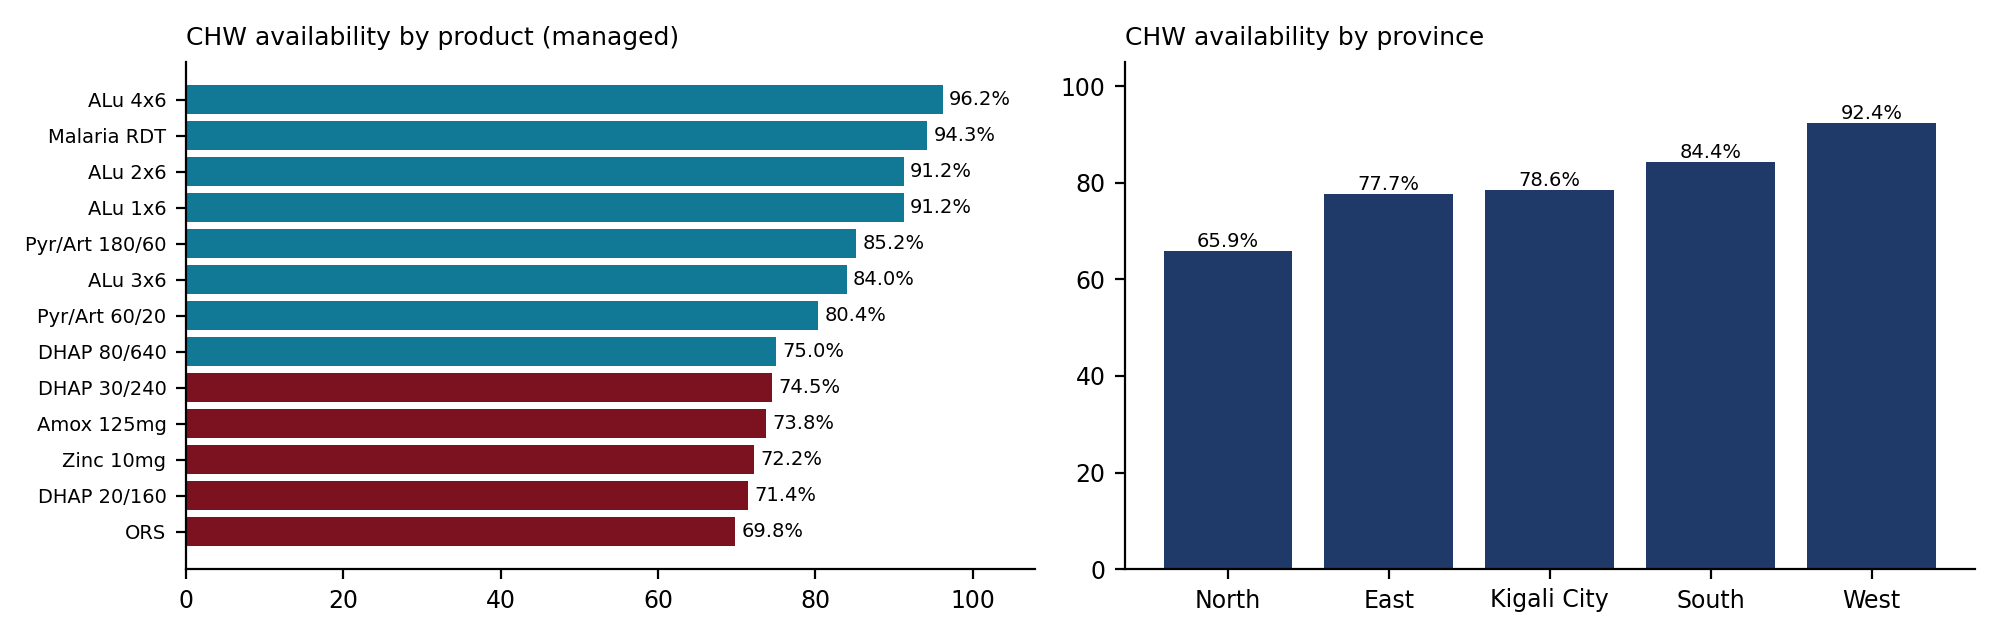
\includegraphics[width=0.96\linewidth]{d6_chw.png}\caption{CHW availability by product and by province.}\end{figure}
{\footnotesize\setlength{\tabcolsep}{3pt}\renewcommand{\arraystretch}{1.15}
\begin{longtable}{>{\raggedright\arraybackslash}p{0.338\linewidth}>{\raggedright\arraybackslash}p{0.162\linewidth}>{\raggedright\arraybackslash}p{0.162\linewidth}>{\raggedright\arraybackslash}p{0.162\linewidth}>{\raggedright\arraybackslash}p{0.135\linewidth}}
\caption{Availability by CHW product}\\
\rowcolor{navy}\textbf{\color{white}Medicine} & \textbf{\color{white}Managed} & \textbf{\color{white}Available} & \textbf{\color{white}AVAILABLE \%} & \textbf{\color{white}CHWs} \\
\endfirsthead
\rowcolor{navy}\textbf{\color{white}Medicine} & \textbf{\color{white}Managed} & \textbf{\color{white}Available} & \textbf{\color{white}AVAILABLE \%} & \textbf{\color{white}CHWs} \\
\endhead
ORS & 169 & 118 & 69.8\% & 169 \\
\rowcolor{band}DHAP 20/160 & 49 & 35 & 71.4\% & 49 \\
Zinc 10mg & 169 & 122 & 72.2\% & 169 \\
\rowcolor{band}Amox 125mg & 164 & 121 & 73.8\% & 164 \\
DHAP 30/240 & 51 & 38 & 74.5\% & 51 \\
\rowcolor{band}DHAP 80/640 & 48 & 36 & 75.0\% & 48 \\
Pyr/Art 60/20 & 51 & 41 & 80.4\% & 51 \\
\rowcolor{band}ALu 3x6 & 50 & 42 & 84.0\% & 50 \\
Pyr/Art 180/60 & 54 & 46 & 85.2\% & 54 \\
\rowcolor{band}ALu 1x6 & 57 & 52 & 91.2\% & 57 \\
ALu 2x6 & 57 & 52 & 91.2\% & 57 \\
\rowcolor{band}Malaria RDT & 174 & 164 & 94.3\% & 174 \\
ALu 4x6 & 53 & 51 & 96.2\% & 53 \\
\end{longtable}}
{\footnotesize\setlength{\tabcolsep}{3pt}\renewcommand{\arraystretch}{1.15}
\begin{longtable}{>{\raggedright\arraybackslash}p{0.686\linewidth}>{\raggedright\arraybackslash}p{0.274\linewidth}}
\caption{Complete CHW basket availability}\\
\rowcolor{navy}\textbf{\color{white}Measure} & \textbf{\color{white}Value} \\
\endfirsthead
\rowcolor{navy}\textbf{\color{white}Measure} & \textbf{\color{white}Value} \\
\endhead
CHWs with a complete assessment & 175 \\
\rowcolor{band}CHWs holding EVERY medicine they manage & 69 \\
COMPLETE BASKET AVAILABILITY & 39.4\% \\
\rowcolor{band}CHWs missing exactly one & 43 \\
CHWs missing three or more & 31 \\
\end{longtable}}
\begin{figure}[H]\centering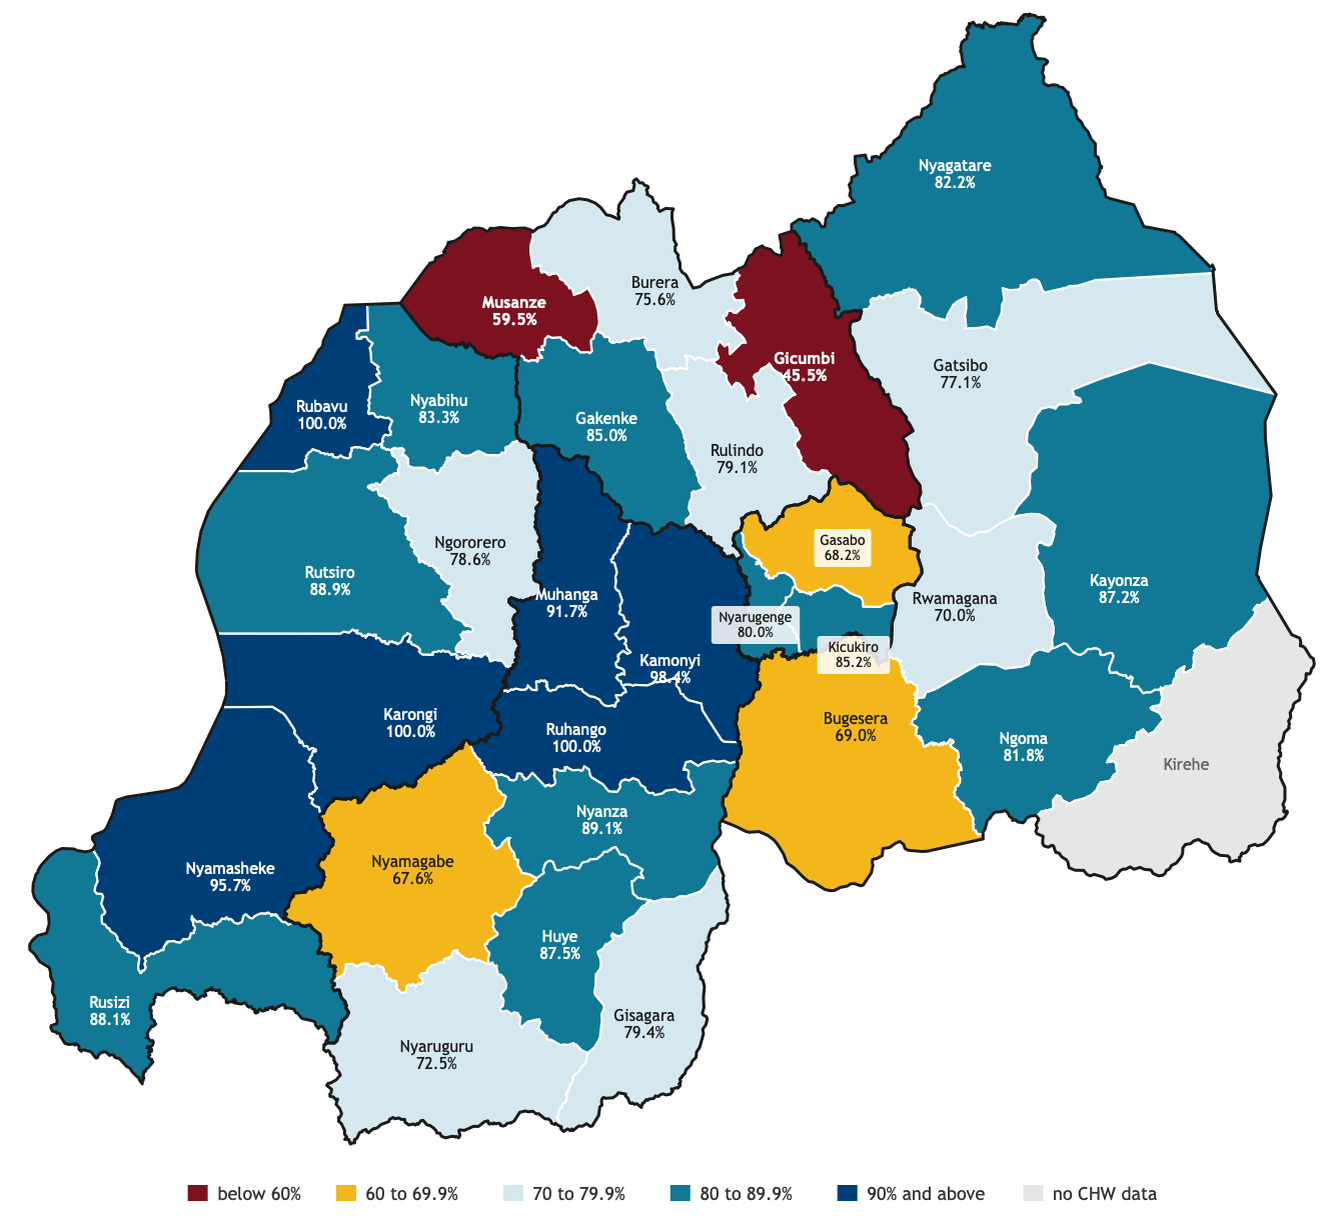
\includegraphics[width=0.66\linewidth]{map_chw.png}\caption{CHW availability by district.}\end{figure}
{\footnotesize\setlength{\tabcolsep}{3pt}\renewcommand{\arraystretch}{1.15}
\begin{longtable}{>{\raggedright\arraybackslash}p{0.204\linewidth}>{\raggedright\arraybackslash}p{0.144\linewidth}>{\raggedright\arraybackslash}p{0.144\linewidth}>{\raggedright\arraybackslash}p{0.156\linewidth}>{\raggedright\arraybackslash}p{0.156\linewidth}>{\raggedright\arraybackslash}p{0.156\linewidth}}
\caption{Community against facility on the products both carry}\\
\rowcolor{navy}\textbf{\color{white}Product} & \textbf{\color{white}CHW observations} & \textbf{\color{white}CHW available \%} & \textbf{\color{white}Facility observations} & \textbf{\color{white}Facility available \%} & \textbf{\color{white}Difference (percentage points)} \\
\endfirsthead
\rowcolor{navy}\textbf{\color{white}Product} & \textbf{\color{white}CHW observations} & \textbf{\color{white}CHW available \%} & \textbf{\color{white}Facility observations} & \textbf{\color{white}Facility available \%} & \textbf{\color{white}Difference (percentage points)} \\
\endhead
ALu 1x6 & 57 & 91.2\% & 92 & 100.0\% & -8.8 pts \\
\rowcolor{band}ALu 4x6 & 53 & 96.2\% & 114 & 100.0\% & -3.8 pts \\
Malaria RDT & 174 & 94.3\% & 253 & 99.2\% & -5.0 pts \\
\rowcolor{band}DHAP 20/160 & 49 & 71.4\% & 67 & 98.5\% & -27.1 pts \\
DHAP 30/240 & 51 & 74.5\% & 79 & 100.0\% & -25.5 pts \\
\rowcolor{band}DHAP 80/640 & 48 & 75.0\% & 67 & 100.0\% & -25.0 pts \\
Pyr/Art 180/60 & 54 & 85.2\% & 97 & 100.0\% & -14.8 pts \\
\rowcolor{band}Pyr/Art 60/20 & 51 & 80.4\% & 97 & 100.0\% & -19.6 pts \\
ALL EIGHT SHARED PRODUCTS & 537 & 86.2\% & 866 & 99.7\% & -13.4 pts \\
\end{longtable}}
The denominator excludes products the CHW does not manage (842 rows, about 42\%), mostly MFT zoning, which is policy rather than a stock-out. ORS, DHAP, zinc and amoxicillin are the least available products; North (65.9\%) lags while the West reaches 92.4\%.

\section{Inferential findings}
\subsection{Treatment readiness and the health centre-to-CHW link}
{\footnotesize\setlength{\tabcolsep}{3pt}\renewcommand{\arraystretch}{1.15}
\begin{longtable}{>{\raggedright\arraybackslash}p{0.508\linewidth}>{\raggedright\arraybackslash}p{0.452\linewidth}}
\caption{CHW treatment readiness by iCCM condition}\\
\rowcolor{navy}\textbf{\color{white}Condition} & \textbf{\color{white}CHWs ready (95\% CI)} \\
\endfirsthead
\rowcolor{navy}\textbf{\color{white}Condition} & \textbf{\color{white}CHWs ready (95\% CI)} \\
\endhead
Malaria (RDT + an ACT) & 84.6\% (79.3-89.9) \\
\rowcolor{band}Malaria (RDT + every managed ACT) & 68.0\% (61.0-75.0) \\
Diarrhoea (ORS + zinc) & 55.4\% (48.1-62.8) \\
\rowcolor{band}Pneumonia (amoxicillin) & 69.1\% (62.2-76.1) \\
All three conditions & 39.4\% (32.1-46.7) \\
\end{longtable}}
{\footnotesize\setlength{\tabcolsep}{3pt}\renewcommand{\arraystretch}{1.15}
\begin{longtable}{>{\raggedright\arraybackslash}p{0.237\linewidth}>{\raggedright\arraybackslash}p{0.181\linewidth}>{\raggedright\arraybackslash}p{0.181\linewidth}>{\raggedright\arraybackslash}p{0.181\linewidth}>{\raggedright\arraybackslash}p{0.181\linewidth}}
\caption{CHW readiness by province}\\
\rowcolor{navy}\textbf{\color{white}Province} & \textbf{\color{white}Malaria} & \textbf{\color{white}Diarrhoea} & \textbf{\color{white}Pneumonia} & \textbf{\color{white}All three} \\
\endfirsthead
\rowcolor{navy}\textbf{\color{white}Province} & \textbf{\color{white}Malaria} & \textbf{\color{white}Diarrhoea} & \textbf{\color{white}Pneumonia} & \textbf{\color{white}All three} \\
\endhead
East & 87.0 & 45.7 & 73.9 & 34.8 \\
\rowcolor{band}Kigali City & 86.7 & 40.0 & 33.3 & 13.3 \\
North & 67.6 & 50.0 & 64.7 & 26.5 \\
\rowcolor{band}South & 93.9 & 61.2 & 75.5 & 51.0 \\
West & 83.9 & 74.2 & 74.2 & 54.8 \\
\multicolumn{5}{p{0.96\linewidth}}{\scriptsize\itshape\color{gray} Percent of CHWs ready.}\\
\end{longtable}}
{\footnotesize\setlength{\tabcolsep}{3pt}\renewcommand{\arraystretch}{1.15}
\begin{longtable}{>{\raggedright\arraybackslash}p{0.282\linewidth}>{\raggedright\arraybackslash}p{0.102\linewidth}>{\raggedright\arraybackslash}p{0.147\linewidth}>{\raggedright\arraybackslash}p{0.169\linewidth}>{\raggedright\arraybackslash}p{0.158\linewidth}>{\raggedright\arraybackslash}p{0.102\linewidth}}
\caption{CHW against supervising health centre on the same product}\\
\rowcolor{navy}\textbf{\color{white}Product (molecule)} & \textbf{\color{white}Pairs} & \textbf{\color{white}CHW available} & \textbf{\color{white}Health centre available} & \textbf{\color{white}CHW out, HC has it} & \textbf{\color{white}McNemar p} \\
\endfirsthead
\rowcolor{navy}\textbf{\color{white}Product (molecule)} & \textbf{\color{white}Pairs} & \textbf{\color{white}CHW available} & \textbf{\color{white}Health centre available} & \textbf{\color{white}CHW out, HC has it} & \textbf{\color{white}McNemar p} \\
\endhead
arte & 52 & 98.1\% & 100.0\% & 1 & 1.000 \\
\rowcolor{band}dihydroartemisinin piperaquine & 57 & 87.7\% & 100.0\% & 7 & 0.016 \\
Malaria RDT & 170 & 94.1\% & 100.0\% & 10 & 0.002 \\
\rowcolor{band}pyronaridine artesunate & 56 & 89.3\% & 100.0\% & 6 & 0.031 \\
\multicolumn{6}{p{0.96\linewidth}}{\scriptsize\itshape\color{gray} CHW paired with the supervising health centre on the same molecule.}\\
\end{longtable}}
\textbf{Interpretation.} Treatment readiness is lower than product availability suggests: only 39.4\% of CHWs could treat malaria, diarrhoea and pneumonia on the visit day, below the 49\% SC4CCM baseline for Rwanda [Chandani 2014] although the product lists differ. Diarrhoea is the weakest condition because ORS and zinc must both be present. Kigali City has the lowest readiness, largely because of amoxicillin. In all 335 CHW-health centre pairs, the health centre had the product whenever the CHW did, and in every one of the 24 discordant pairs the CHW was out while the health centre had stock (exact p $<$0.001). The community gap is therefore one of resupply from the health centre to the CHW, which also matches the Bugesera finding that CHWs walk and pay to collect stock [Gakinahe 2024].

\chapter{Cross-cutting analyses}
\section{Precision and representativeness of the estimates}
{\footnotesize\setlength{\tabcolsep}{3pt}\renewcommand{\arraystretch}{1.15}
\begin{longtable}{>{\raggedright\arraybackslash}p{0.316\linewidth}>{\raggedright\arraybackslash}p{0.175\linewidth}>{\raggedright\arraybackslash}p{0.175\linewidth}>{\raggedright\arraybackslash}p{0.175\linewidth}>{\raggedright\arraybackslash}p{0.119\linewidth}}
\caption{Headline indicators: pooled and weighted estimates with 95\% confidence intervals}\\
\rowcolor{navy}\textbf{\color{white}Indicator} & \textbf{\color{white}Pooled (95\% CI)} & \textbf{\color{white}Weighted (95\% CI)} & \textbf{\color{white}Weighted, no HP} & \textbf{\color{white}Design effect} \\
\endfirsthead
\rowcolor{navy}\textbf{\color{white}Indicator} & \textbf{\color{white}Pooled (95\% CI)} & \textbf{\color{white}Weighted (95\% CI)} & \textbf{\color{white}Weighted, no HP} & \textbf{\color{white}Design effect} \\
\endhead
Availability, expected medicines (M1) & 87.8\% (87.0-88.6) & 77.7\% (75.8-79.6) & 88.7\% (87.8-89.5) & 1.5 \\
\rowcolor{band}Availability, managed products (M2) & 93.7\% (92.9-94.4) & 93.0\% (90.8-95.3) & 93.6\% (92.9-94.4) & 2.1 \\
Stock-out incidence, Jun-Aug & 9.7\% (8.6-10.8) & 8.9\% (6.4-11.4) & 10.0\% (8.8-11.1) & 3.5 \\
\rowcolor{band}Stocked out on the visit day & 7.0\% (6.1-7.8) & 8.0\% (5.1-10.9) & 7.0\% (6.1-7.9) & 2.5 \\
Understocked ($<$1 month) & 22.3\% (20.7-23.9) & 19.5\% (16.8-22.2) & 22.1\% (20.4-23.8) & 3.2 \\
\rowcolor{band}Adequately stocked (1-2 months) & 24.6\% (23.4-25.7) & 24.2\% (21.7-26.7) & 24.3\% (23.1-25.6) & 1.7 \\
Overstocked ($>$2 months) & 46.2\% (44.3-48.0) & 48.3\% (44.6-52.0) & 46.6\% (44.6-48.5) & 3.1 \\
\rowcolor{band}Inventory record accuracy (exact match) & 56.1\% (51.6-60.6) & 46.5\% (36.8-56.2) & 55.1\% (50.3-59.9) & 19.1 \\
Order fill rate (quantity) & 93.1\% (91.0-95.2) & 93.0\% (91.1-94.9) & 93.0\% (90.9-95.0) & - \\
\rowcolor{band}CHW product availability (managed) & 80.1\% (76.8-83.4) & - & - & 2.1 \\
Prescriptions fully served & 98.8\% (98.0-99.6) & 99.6\% (99.2-99.9) & - & 9.2 \\
\rowcolor{band}Prescribed items unserved & 0.8\% (0.1-1.4) & 0.3\% (0.0-0.5) & - & 18.1 \\
\multicolumn{5}{p{0.96\linewidth}}{\scriptsize\itshape\color{gray} Pooled = as on the dashboard. Weighted = weighted by level to the national facility register. Design effect = variance relative to simple random sampling.}\\
\end{longtable}}
\begin{figure}[H]\centering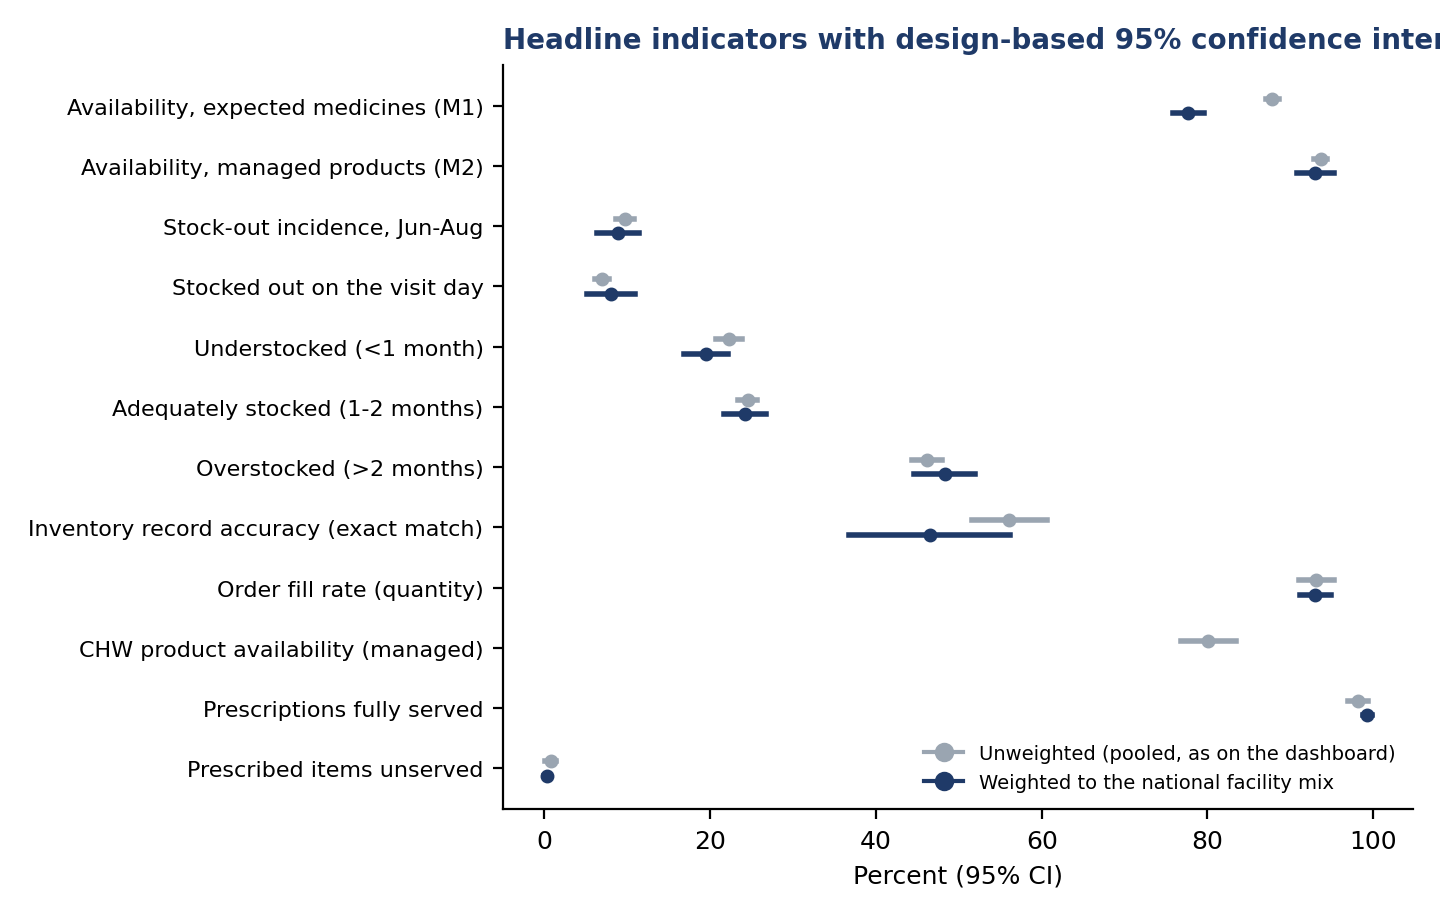
\includegraphics[width=0.96\linewidth]{fig_estimates.png}\caption{Headline indicators with 95\% confidence intervals.}\end{figure}
\textbf{Interpretation.} The pooled figures on the dashboard are precise: the 95\% intervals for availability are about $\pm$1 point. Weighting changes the picture for expected-medicine availability (87.8\% pooled, 77.7\% weighted), because health posts make up most of Rwanda's facilities and stock fewer of the medicines the EML authorises for them; without health posts the weighted value (88.7\%) is close to the pooled one. Managed-product availability is robust to weighting. Record accuracy has a design effect of 19.1: accuracy is mostly a property of the facility, so its interval (51.6-60.6\%) is much wider than the 8,856 records would suggest, and its weighted value (46.5\%) is lower because health posts keep the least accurate records. The prescription indicators are very precise but, as noted on the dashboard, understate unmet need by design.

\section{Which group differences are statistically robust}
{\footnotesize\setlength{\tabcolsep}{3pt}\renewcommand{\arraystretch}{1.15}
\begin{longtable}{>{\raggedright\arraybackslash}p{0.276\linewidth}>{\raggedright\arraybackslash}p{0.276\linewidth}>{\raggedright\arraybackslash}p{0.276\linewidth}>{\raggedright\arraybackslash}p{0.132\linewidth}}
\caption{Managed availability and stock-out incidence by level of care (95\% CI)}\\
\rowcolor{navy}\textbf{\color{white}Level of care} & \textbf{\color{white}Managed availability \% (95\% CI)} & \textbf{\color{white}Stock-out incidence \% (95\% CI)} & \textbf{\color{white}Facilities} \\
\endfirsthead
\rowcolor{navy}\textbf{\color{white}Level of care} & \textbf{\color{white}Managed availability \% (95\% CI)} & \textbf{\color{white}Stock-out incidence \% (95\% CI)} & \textbf{\color{white}Facilities} \\
\endhead
District hospital & 96.7 (95.1-98.4) & 5.6 (3.2-8.0) & 24 \\
\rowcolor{band}Health centre & 93.4 (92.6-94.3) & 10.3 (9.0-11.6) & 205 \\
Health post & 92.6 (88.6-96.5) & 8.1 (3.8-12.4) & 25 \\
\rowcolor{band}Level 2 teaching hospital & 91.9 (88.7-95.1) & 10.6 (5.6-15.5) & 10 \\
National referral hospital & 93.0 (92.4-93.7) & 14.0 (-1.0-28.9) & 2 \\
\end{longtable}}
{\footnotesize\setlength{\tabcolsep}{3pt}\renewcommand{\arraystretch}{1.15}
\begin{longtable}{>{\raggedright\arraybackslash}p{0.276\linewidth}>{\raggedright\arraybackslash}p{0.276\linewidth}>{\raggedright\arraybackslash}p{0.276\linewidth}>{\raggedright\arraybackslash}p{0.132\linewidth}}
\caption{Managed availability and stock-out incidence by management type (95\% CI)}\\
\rowcolor{navy}\textbf{\color{white}Management type} & \textbf{\color{white}Managed availability \% (95\% CI)} & \textbf{\color{white}Stock-out incidence \% (95\% CI)} & \textbf{\color{white}Facilities} \\
\endfirsthead
\rowcolor{navy}\textbf{\color{white}Management type} & \textbf{\color{white}Managed availability \% (95\% CI)} & \textbf{\color{white}Stock-out incidence \% (95\% CI)} & \textbf{\color{white}Facilities} \\
\endhead
Faith based facility based & 95.0 (93.8-96.3) & 7.9 (5.8-9.9) & 72 \\
\rowcolor{band}Government & 93.3 (92.4-94.2) & 10.4 (9.0-11.8) & 167 \\
PPP & 92.1 (88.4-95.8) & 8.7 (4.6-12.7) & 26 \\
\end{longtable}}
{\footnotesize\setlength{\tabcolsep}{3pt}\renewcommand{\arraystretch}{1.15}
\begin{longtable}{>{\raggedright\arraybackslash}p{0.276\linewidth}>{\raggedright\arraybackslash}p{0.276\linewidth}>{\raggedright\arraybackslash}p{0.276\linewidth}>{\raggedright\arraybackslash}p{0.132\linewidth}}
\caption{Managed availability and stock-out incidence by province (95\% CI)}\\
\rowcolor{navy}\textbf{\color{white}Province} & \textbf{\color{white}Managed availability \% (95\% CI)} & \textbf{\color{white}Stock-out incidence \% (95\% CI)} & \textbf{\color{white}Facilities} \\
\endfirsthead
\rowcolor{navy}\textbf{\color{white}Province} & \textbf{\color{white}Managed availability \% (95\% CI)} & \textbf{\color{white}Stock-out incidence \% (95\% CI)} & \textbf{\color{white}Facilities} \\
\endhead
East & 93.2 (91.8-94.6) & 11.2 (8.7-13.7) & 65 \\
\rowcolor{band}Kigali City & 94.8 (93.5-96.0) & 7.3 (5.3-9.3) & 26 \\
North & 93.1 (91.1-95.0) & 10.7 (8.4-13.1) & 50 \\
\rowcolor{band}South & 94.9 (93.6-96.2) & 8.1 (5.8-10.4) & 71 \\
West & 92.7 (90.8-94.6) & 9.9 (7.7-12.2) & 54 \\
\end{longtable}}
{\footnotesize\setlength{\tabcolsep}{3pt}\renewcommand{\arraystretch}{1.15}
\begin{longtable}{>{\raggedright\arraybackslash}p{0.276\linewidth}>{\raggedright\arraybackslash}p{0.276\linewidth}>{\raggedright\arraybackslash}p{0.276\linewidth}>{\raggedright\arraybackslash}p{0.132\linewidth}}
\caption{Managed availability and stock-out incidence by RMS hub (95\% CI)}\\
\rowcolor{navy}\textbf{\color{white}Rms hub} & \textbf{\color{white}Managed availability \% (95\% CI)} & \textbf{\color{white}Stock-out incidence \% (95\% CI)} & \textbf{\color{white}Facilities} \\
\endfirsthead
\rowcolor{navy}\textbf{\color{white}Rms hub} & \textbf{\color{white}Managed availability \% (95\% CI)} & \textbf{\color{white}Stock-out incidence \% (95\% CI)} & \textbf{\color{white}Facilities} \\
\endhead
Huye HUB & 95.3 (93.9-96.7) & 8.6 (5.9-11.2) & 61 \\
\rowcolor{band}Karongi HUB & 92.8 (90.4-95.2) & 9.7 (6.7-12.8) & 35 \\
Kayonza HUB & 93.8 (92.3-95.4) & 10.2 (7.4-12.9) & 55 \\
\rowcolor{band}Kigali HUB & 92.4 (91.0-93.7) & 9.3 (7.5-11.2) & 66 \\
Musanze HUB & 93.8 (92.0-95.6) & 10.9 (8.6-13.2) & 49 \\
\end{longtable}}
\textbf{Interpretation.} Overlapping intervals mean many apparent differences on the dashboard are within sampling error. Of the 30 districts, 5 have managed availability significantly below the national value (Gicumbi, Ngoma, Gakenke, Bugesera, Rubavu) and 9 significantly above (Kicukiro, Gisagara, Nyanza, Huye, Muhanga, Nyamasheke, Musanze, Rwamagana, Burera); the remaining 16 cannot be distinguished from the national figure with 5-11 facilities each. District maps should be read with this in mind.

\section{Where the variation lies}
{\footnotesize\setlength{\tabcolsep}{3pt}\renewcommand{\arraystretch}{1.15}
\begin{longtable}{>{\raggedright\arraybackslash}p{0.305\linewidth}>{\raggedright\arraybackslash}p{0.215\linewidth}>{\raggedright\arraybackslash}p{0.215\linewidth}>{\raggedright\arraybackslash}p{0.226\linewidth}}
\caption{Variance partition: share of variation between facilities and districts}\\
\rowcolor{navy}\textbf{\color{white}Outcome} & \textbf{\color{white}Between facilities} & \textbf{\color{white}Between districts} & \textbf{\color{white}Within facility (residual)} \\
\endfirsthead
\rowcolor{navy}\textbf{\color{white}Outcome} & \textbf{\color{white}Between facilities} & \textbf{\color{white}Between districts} & \textbf{\color{white}Within facility (residual)} \\
\endhead
Available on the visit day & 9.8\% & 3.3\% & 86.9\% \\
\rowcolor{band}Any stock-out day, Jun-Aug & 10.4\% & 6.5\% & 83.0\% \\
Exact record match & 50.0\% & 23.3\% & 26.7\% \\
\multicolumn{4}{p{0.96\linewidth}}{\scriptsize\itshape\color{gray} Variance partition from random-intercept logistic models (latent scale).}\\
\end{longtable}}
\textbf{Interpretation.} For availability and stock-outs, most variation is between medicines within the same facility; facilities and districts explain only 13.1\% and 16.9\%. Stock problems are therefore mostly medicine-specific, and national or programme-level supply actions matter as much as facility mentorship. Record accuracy is the opposite: 50.0\% of its variation is between facilities and 23.3\% between districts. A facility either keeps its records reconciled or it does not, which makes accuracy a natural target for facility-level QMIA mentorship.

\section{Geographic clustering}
{\footnotesize\setlength{\tabcolsep}{3pt}\renewcommand{\arraystretch}{1.15}
\begin{longtable}{>{\raggedright\arraybackslash}p{0.339\linewidth}>{\raggedright\arraybackslash}p{0.169\linewidth}>{\raggedright\arraybackslash}p{0.254\linewidth}>{\raggedright\arraybackslash}p{0.198\linewidth}}
\caption{Spatial autocorrelation of district indicators (Moran's I)}\\
\rowcolor{navy}\textbf{\color{white}District indicator} & \textbf{\color{white}Moran's I} & \textbf{\color{white}Expected under no clustering} & \textbf{\color{white}Permutation p} \\
\endfirsthead
\rowcolor{navy}\textbf{\color{white}District indicator} & \textbf{\color{white}Moran's I} & \textbf{\color{white}Expected under no clustering} & \textbf{\color{white}Permutation p} \\
\endhead
M2 availability & -0.092 & -0.034 & 0.668 \\
\rowcolor{band}M1 availability & -0.078 & -0.034 & 0.633 \\
Stock-out incidence & -0.179 & -0.034 & 0.924 \\
\rowcolor{band}Record accuracy & -0.072 & -0.034 & 0.596 \\
CHW availability & 0.152 & -0.036 & 0.050 \\
\end{longtable}}
\textbf{Interpretation.} Neighbouring districts are no more alike than distant ones for availability, stock-outs or record accuracy; weak districts are scattered rather than forming a region. CHW availability shows weak positive clustering (p about 0.05), consistent with zone-wide antimalarial allocation. In practice this means support should be allocated facility by facility rather than to a whole region.

\section{Facility profiles for targeting}
{\footnotesize\setlength{\tabcolsep}{3pt}\renewcommand{\arraystretch}{1.15}
\begin{longtable}{>{\raggedright\arraybackslash}p{0.260\linewidth}>{\raggedright\arraybackslash}p{0.102\linewidth}>{\raggedright\arraybackslash}p{0.102\linewidth}>{\raggedright\arraybackslash}p{0.096\linewidth}>{\raggedright\arraybackslash}p{0.096\linewidth}>{\raggedright\arraybackslash}p{0.096\linewidth}>{\raggedright\arraybackslash}p{0.102\linewidth}>{\raggedright\arraybackslash}p{0.107\linewidth}}
\caption{Facility profiles from k-means clustering}\\
\rowcolor{navy}\textbf{\color{white}Profile} & \textbf{\color{white}Facilities} & \textbf{\color{white}Availability} & \textbf{\color{white}Stock-out} & \textbf{\color{white}Accuracy} & \textbf{\color{white}Fill rate} & \textbf{\color{white}Overstock} & \textbf{\color{white}Understock} \\
\endfirsthead
\rowcolor{navy}\textbf{\color{white}Profile} & \textbf{\color{white}Facilities} & \textbf{\color{white}Availability} & \textbf{\color{white}Stock-out} & \textbf{\color{white}Accuracy} & \textbf{\color{white}Fill rate} & \textbf{\color{white}Overstock} & \textbf{\color{white}Understock} \\
\endhead
1. Well supplied but overstocked & 92 & 96.8 & 5.7 & 55.6 & 96.1 & 62.4 & 10.1 \\
\rowcolor{band}2. Weak resupply and weak records & 35 & 93.0 & 10.3 & 40.4 & 77.1 & 46.8 & 22.8 \\
3. Frequent stock-outs & 54 & 85.6 & 21.9 & 59.9 & 96.5 & 34.8 & 25.7 \\
\rowcolor{band}4. Lean stock, often understocked & 85 & 95.9 & 5.5 & 55.2 & 97.1 & 37.0 & 31.8 \\
\multicolumn{8}{p{0.96\linewidth}}{\scriptsize\itshape\color{gray} Cluster means, percent. The facility list is in results/facility\_typology.csv.}\\
\end{longtable}}
\begin{figure}[H]\centering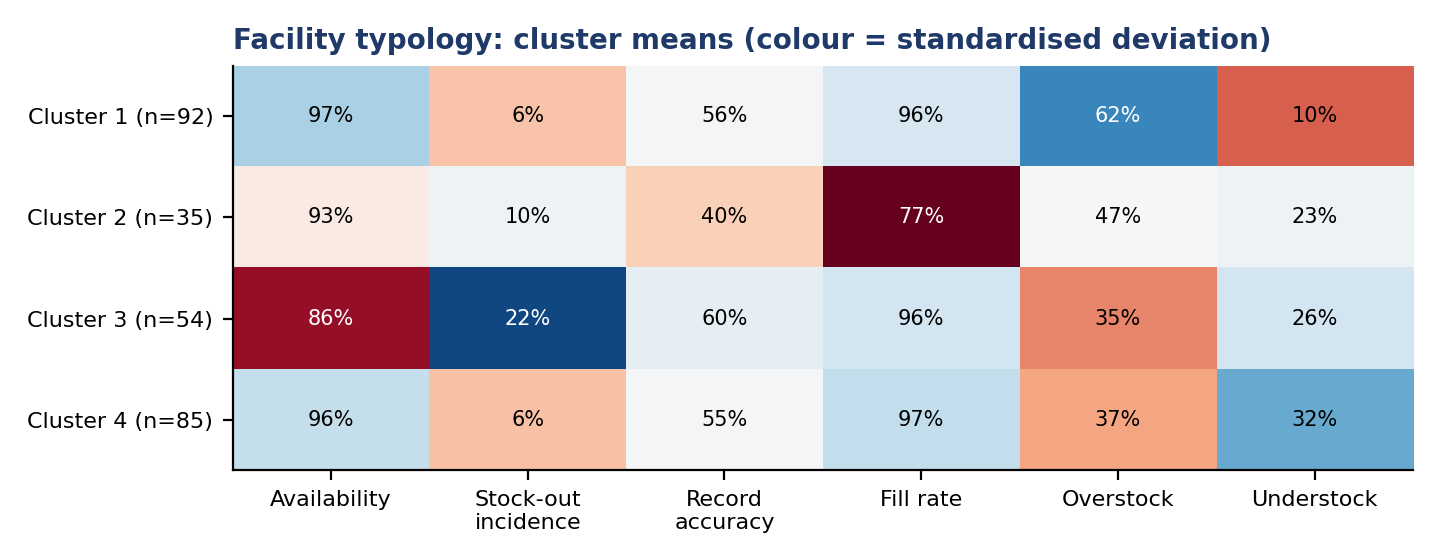
\includegraphics[width=0.90\linewidth]{fig_typology.png}\caption{Facility profiles from k-means clustering.}\end{figure}
\textbf{Interpretation.} The profiles separate problems that need different responses. \textbf{Frequent stock-outs} facilities have the lowest availability despite normal fill rates, pointing to under-ordering and quantification. \textbf{Weak resupply and weak records} facilities receive markedly less of what they order and keep the least accurate records; they need RMS follow-up and record reconciliation together. \textbf{Well supplied but overstocked} facilities are candidates for redistribution of excess stock. \textbf{Lean stock, often understocked} facilities run close to the emergency order point and need more frequent resupply. The silhouette values are modest, so the profiles are a practical grouping for planning rather than sharply distinct types.

\section{Predicting stock-outs}
{\footnotesize\setlength{\tabcolsep}{3pt}\renewcommand{\arraystretch}{1.15}
\begin{longtable}{>{\raggedright\arraybackslash}p{0.339\linewidth}>{\raggedright\arraybackslash}p{0.248\linewidth}>{\raggedright\arraybackslash}p{0.186\linewidth}>{\raggedright\arraybackslash}p{0.186\linewidth}}
\caption{Predictive model performance (facility-grouped cross-validation)}\\
\rowcolor{navy}\textbf{\color{white}Model} & \textbf{\color{white}AUC (95\% CI)} & \textbf{\color{white}Average precision} & \textbf{\color{white}Brier score} \\
\endfirsthead
\rowcolor{navy}\textbf{\color{white}Model} & \textbf{\color{white}AUC (95\% CI)} & \textbf{\color{white}Average precision} & \textbf{\color{white}Brier score} \\
\endhead
A: Logistic regression & 0.901 (0.884-0.917) & 0.670 & 0.0324 \\
\rowcolor{band}A: Random forest & 0.904 (0.888-0.920) & 0.724 & 0.0311 \\
A: Gradient boosting & 0.905 (0.887-0.920) & 0.702 & 0.0323 \\
\rowcolor{band}B: Logistic regression & 0.878 (0.848-0.904) & 0.622 & 0.0318 \\
B: Random forest & 0.896 (0.875-0.921) & 0.674 & 0.0307 \\
\rowcolor{band}B: Gradient boosting & 0.887 (0.869-0.905) & 0.650 & 0.0313 \\
\multicolumn{4}{p{0.96\linewidth}}{\scriptsize\itshape\color{gray} A: stock-out in August (prevalence 6.9\%). B: unavailable on the visit day (prevalence 6.1\%). Facility-grouped five-fold cross-validation.}\\
\end{longtable}}
\begin{figure}[H]\centering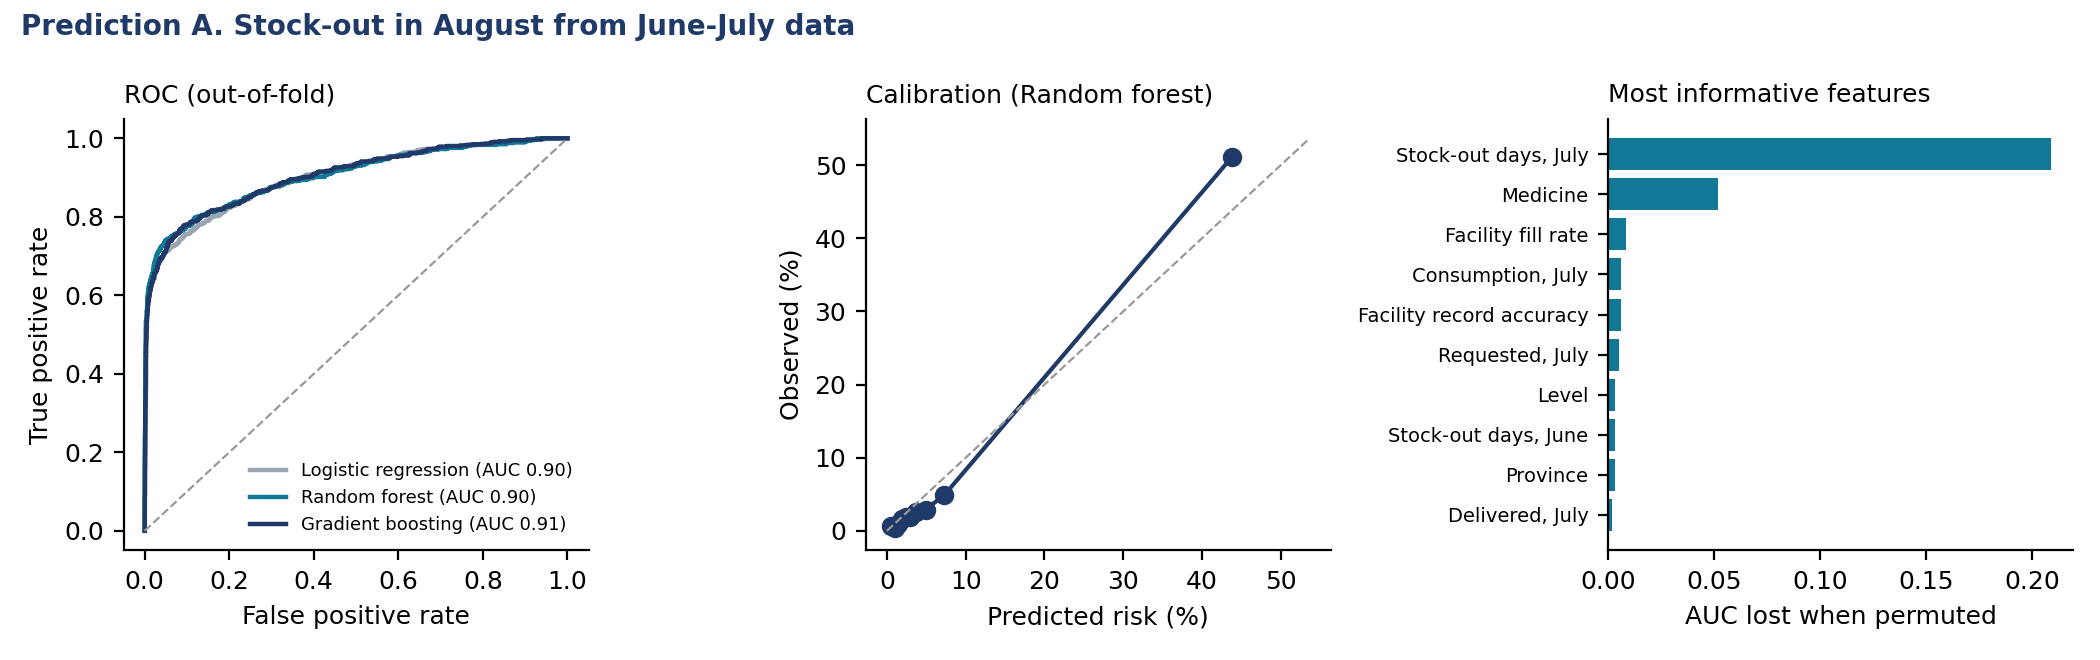
\includegraphics[width=0.96\linewidth]{fig_pred_august.png}\caption{Prediction A: ROC, calibration and feature importance.}\end{figure}
\begin{figure}[H]\centering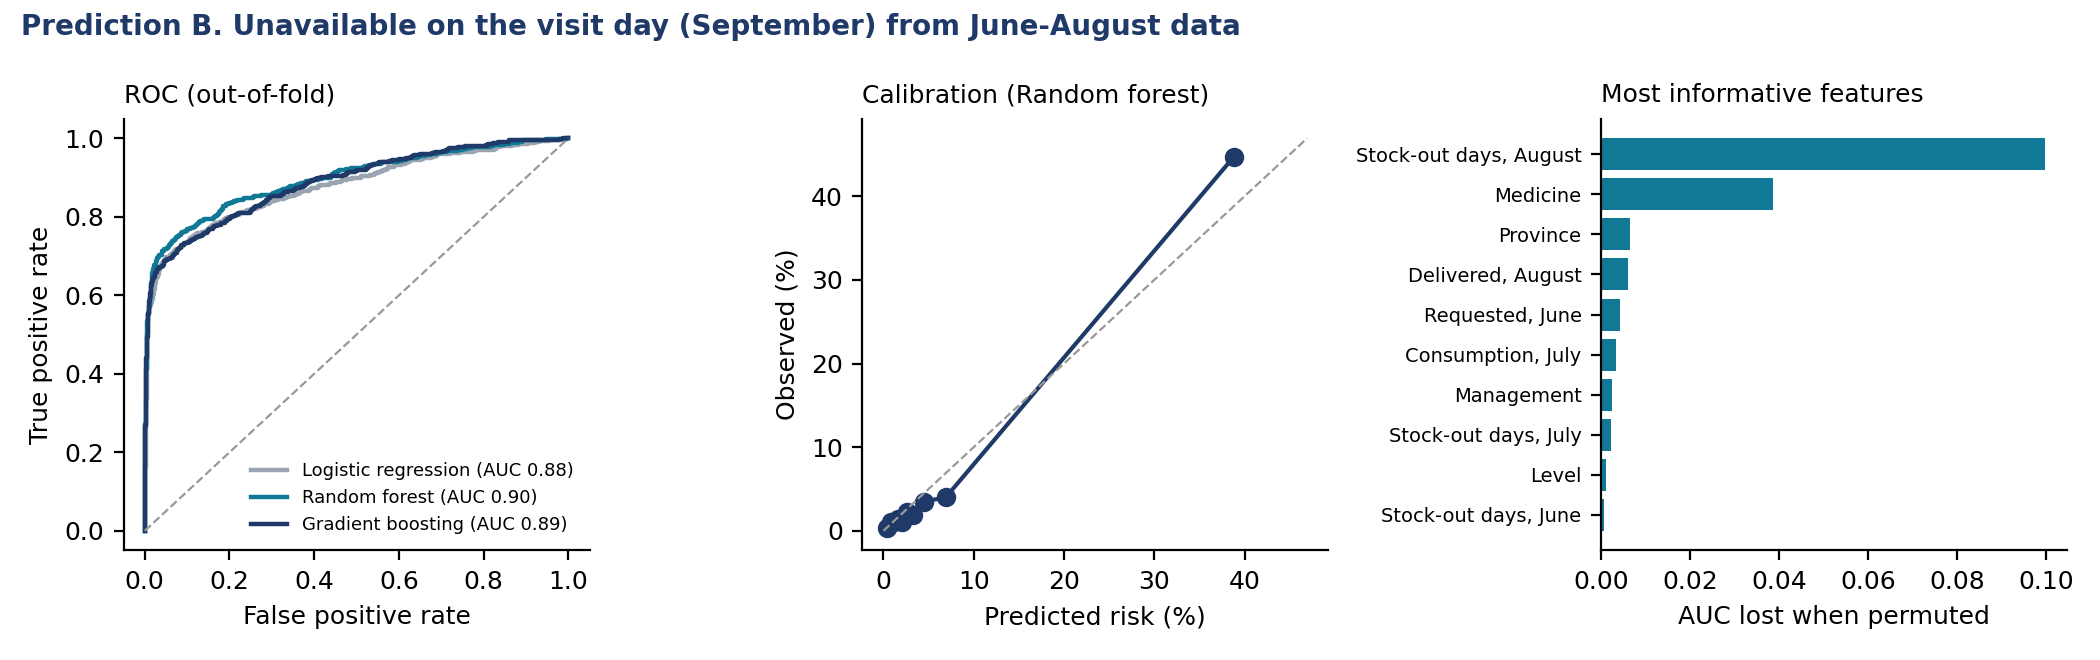
\includegraphics[width=0.96\linewidth]{fig_pred_visit.png}\caption{Prediction B: ROC, calibration and feature importance.}\end{figure}
{\footnotesize\setlength{\tabcolsep}{3pt}\renewcommand{\arraystretch}{1.15}
\begin{longtable}{>{\raggedright\arraybackslash}p{0.395\linewidth}>{\raggedright\arraybackslash}p{0.181\linewidth}>{\raggedright\arraybackslash}p{0.181\linewidth}>{\raggedright\arraybackslash}p{0.203\linewidth}}
\caption{Early-warning operating points: model against a simple rule}\\
\rowcolor{navy}\textbf{\color{white}Approach} & \textbf{\color{white}Pairs flagged} & \textbf{\color{white}Precision} & \textbf{\color{white}Recall} \\
\endfirsthead
\rowcolor{navy}\textbf{\color{white}Approach} & \textbf{\color{white}Pairs flagged} & \textbf{\color{white}Precision} & \textbf{\color{white}Recall} \\
\endhead
A: rule ''out in July'' & 6.3\% & 72.8\% & 66.7\% \\
\rowcolor{band}A: Random forest, same flag rate & 6.3\% & 71.6\% & 65.7\% \\
A: Random forest, top 10\% risk & 10.0\% & 51.1\% & 74.1\% \\
\rowcolor{band}B: rule ''out in July'' & 6.3\% & 49.2\% & 50.8\% \\
B: Random forest, same flag rate & 6.3\% & 65.5\% & 67.6\% \\
\rowcolor{band}B: Random forest, top 10\% risk & 10.0\% & 44.7\% & 73.1\% \\
\multicolumn{4}{p{0.96\linewidth}}{\scriptsize\itshape\color{gray} Precision: share of flagged pairs that stocked out. Recall: share of stock-outs flagged.}\\
\end{longtable}}
\textbf{Interpretation.} All three models discriminate well (AUC about 0.90 for August stock-outs and 0.90 for the visit day), and the random forest is well calibrated. Most of this comes from persistence: July stock-out days are by far the most informative feature, and for August the simple rule ''flag what was out in July'' performs as well as the model at the same flag rate. The models add value in two ways. First, they rank risk among pairs that were not out in July (AUC 0.73 for new August stock-outs; 0.81 for the visit day), using the medicine, consumption, requests and the facility's fill rate and record accuracy. Second, for the visit-day outcome the model beats the rule clearly at the same flag rate (precision 65.5\% against 49.2\%). Flagging the top 10\% of pairs by predicted risk captures about 74.1\% of next-month stock-outs with a 7.4-fold lift over random selection. A monthly early-warning list built from eLMIS data in this way is feasible; it should be validated on a later period before use, because three months is a short history.

\chapter{Discussion}
\section{Main messages}
\begin{itemize}\item \textbf{Availability is high by regional standards but uneven.} The managed-product figure (93.7\%) and the expected-medicine figure (87.8\%) are well above typical African public-sector values. The national weighted figure for expected medicines (77.7\%) is lower because health posts, which are most of Rwanda's facilities, do not stock many of the medicines the EML authorises for them.
\item \textbf{Order fulfilment is a lever with a measurable effect.} Nil-filled requisitions multiply the odds of next-month stock-out about 7.6-fold. This is the most actionable result for RMS, and it echoes evidence that order fulfilment and inventory policy, more than facility traits, drive stock-outs [Leung 2016; Mohan 2024].
\item \textbf{Stock problems are medicine- and pipeline-specific.} Facilities and districts explain little of the variation in availability and stock-outs, and there is no regional clustering. National quantification for the essential-medicines pipeline (insulin, thiamine, HIV test kits, paediatric RHZ) matters as much as facility mentorship.
\item \textbf{Record accuracy is the facility-level weakness, and it has slipped.} 56.1\% exact match is well below the 85\% QMIA reported for 2019 [Kigenza 2023], and eBuzima sites are markedly worse. This is where facility mentorship pays off.
\item \textbf{Antibiotic use is the main prescribing concern}, while generic and EML prescribing are excellent.
\item \textbf{The last mile to CHWs is the weak link in community supply.} Health centres hold stock their CHWs lack.
\end{itemize}
\section{Comparison with other studies}
\subsection{Availability of medicines}
Public-sector availability of essential medicines in sub-Saharan Africa has typically been 30-60\% in WHO/HAI surveys [Cameron 2009]. Rwanda has sat at the upper end: 44.2\% mean availability of 32 medicines in the 2007 SPA [Choi and Ametepi 2013], 59.6\% in the public sector and 62.8\% in faith-based facilities in a 2020 WHO/HAI survey of 18 medicines [Bizimana 2020], and 71-78\% for NCD medicines in three rural districts [Mukundiyukuri 2020]. The WHO target is 80\% availability of essential NCD medicines. The QMIA basket and definitions differ (tracer medicines, managed and EML-expected denominators), so our 87.8-93.7\% is not directly comparable, but it is consistent with the improvement reported by QMIA itself [Kigenza 2023].

\subsection{Stock-outs and their determinants}
Day-of-visit stock-out of essential medicines was 18-39\% across levels in Ghana, Kenya and Uganda, worst at the lowest level [Masters 2014]. Recurrent determinants are distance and rurality, facility level, transport, order fulfilment and inventory policy. In Zambia, up to 30\% of clinics stocked out of an artemether-lumefantrine product while the central warehouse had ample stock, which the authors traced to the max-min rule under seasonal demand [Leung 2016]. In Tanzania, facilities with no stock-outs had higher household use of care [Kuwawenaruwa 2020]. A census of 940 Malawian facilities found faith-based ownership (OR 1.63), computerisation (OR 1.46) and more order fulfilments (OR 1.14) associated with availability, and distance over 75 km with lower availability (OR 0.79) [Mohan 2024].

\subsection{Inventory records and eLMIS}
The published evaluation of QMIA in Rwanda reported eLMIS use rising from 55\% to 96\%, inventory accuracy from 25\% to 85\% and the stock-out rate falling from 10\% to 1\% between 2017 and 2019 [Kigenza 2023]. Inventory accuracy of 70-85\% is typical in Ethiopian LIAT-style surveys [Mekonen 2025], and up-to-date bin cards and eLMIS were associated with far fewer stock-outs of emergency obstetric drugs in Rwandan district hospitals [Kabera and Mukanyangezi 2024]. Our exact-match accuracy of 56.1\% is therefore below both the Rwandan 2019 figure and regional benchmarks, although the definitions differ (exact equality here, tolerance bands in some studies).

\subsection{Prescribing}
A review of 43 studies in the WHO African region found median values of 3.1 medicines per encounter, 68\% generic prescribing, 46.8\% of encounters with an antibiotic, 25\% with an injection and 88\% from the EML [Ofori-Asenso 2016], against WHO reference values of under 2 medicines, 100\% generic, under 30\% antibiotic, under 20\% injection and 100\% EML [WHO 1993]. A paediatric study in Burundi reported 2.4 medicines, 78.8\% generic and 9.9\% injection [Manirakiza 2024].

\subsection{Unserved prescriptions}
Direct measurement of unserved prescriptions is rare. In Eswatini, 71\% of chronic-disease patients did not always receive all prescribed medicines and 94\% of them were referred to private pharmacies [Shabangu and Suleman 2015]. No Rwandan study of unserved prescriptions was found; QMIA 2026 appears to be the first national estimate.

\subsection{Community level}
SC4CCM found 49\% of Rwandan CHWs holding all five iCCM products at baseline, rising to 63\% in quality-collaborative districts against 38\% in comparison districts [Chandani 2014], with gains not fully sustained [Chandani 2017]. In Bugesera, self-reported antimalarial stock-out among 295 CHWs was 3.2\%, but most walked to resupply and over half spent their own money doing so [Gakinahe 2024].

\subsection{Prediction}
African work has focused on demand forecasting rather than stock-out classification. A random forest on Rwandan eLMIS data forecast essential-medicine demand with 76\% test accuracy [Mbonyinshuti 2022]. No peer-reviewed African study reporting the discrimination (AUC) of a facility stock-out classifier was found, so the models in Section 4.12 have few direct comparators.

\subsection{Antimalarial zoning}
Rwanda introduced multiple first-line therapies in response to artemisinin partial resistance (kelch13 R561H) [Uwimana 2020; Zupko 2023]. A 2025 description of the deployment plan allocates artesunate-pyronaridine to western districts, dihydroartemisinin-piperaquine to the East and Kigali, and artemether-lumefantrine to the South [Muvunyi 2025]. This differs from the zoning used in cleaning rule S10 for several districts, which reinforces the need to obtain the official district list.

\section{Strengths and limitations}
\begin{itemize}\item \textbf{Strengths:} national coverage of all levels; linked stock, prescription and CHW data; confidence intervals and design effects that account for clustering; a temporally ordered test of order fulfilment; predictive models validated by facility-grouped cross-validation.
\item \textbf{Cross-sectional design.} Except for the lagged panel, associations are not causal.
\item \textbf{Short history.} Three months (June-August) limit trend and prediction; the models should be revalidated on later months.
\item \textbf{Weights.} Health posts were sampled purposively; weighted national figures that include them should be read as indicative.
\item \textbf{Self-report.} RMS availability and some quantities are facility-reported; consumption may be under-recorded where dispensing is not captured.
\item \textbf{Prescription design.} Prescribers write what the pharmacy holds, so unserved rates understate unmet need; there is no outpatient/inpatient flag.
\item \textbf{Zoning.} Cleaning rule S10 uses a partly inferred zoning list that differs from the published deployment plan for some districts [Muvunyi 2025].
\end{itemize}
\begin{itemize}\item \textbf{Visit-day measurement.} Availability is a single-day snapshot; stock-out history relies on stock cards and records for June-August only (March-May fields were empty).
\item \textbf{Partial RSSB data.} RSSB billing fields cover 215 facilities, mostly health centres.
\item \textbf{CHW sample.} 175 CHWs against 237 planned; Kirehe has no CHW data and no cadre was recorded.
\end{itemize}
\chapter{Recommendations}
\begin{itemize}\item \textbf{RMS: treat a nil-filled order as an alert.} Track requisitions delivered at 0\% and expedite or substitute within the month; report the share monthly by hub.
\item \textbf{Facilities: never skip a requisition cycle} for a managed medicine, even when stock looks sufficient; a missed order raises the odds of a stock-out next month about 2.6-fold.
\item \textbf{Build a monthly stock-out early-warning list} from eLMIS: pairs out last month plus the model's top-risk pairs, sent to RMS branches and district pharmacists.
\item \textbf{Focus QMIA mentorship on record reconciliation} at health centres using eBuzima, and at PPP facilities; aim to restore the 85\% accuracy of 2019.
\item \textbf{Use the facility profiles to tailor support:} redistribution for overstocked sites, RMS follow-up for weak-resupply sites, quantification support for frequent-stock-out sites.
\item \textbf{Strengthen health centre-to-CHW resupply}, especially ORS and zinc as a pair and amoxicillin in Kigali City; consider resupply at the monthly CHW meeting.
\item \textbf{Antimicrobial stewardship in primary care:} feed back antibiotic prescribing rates by facility and prescriber, starting with health centres and general practitioners.
\item \textbf{Report weighted estimates with confidence intervals} in the national report, and flag district values whose intervals include the national figure.
\item \textbf{Confirm the official MFT zoning list} and rerun the zoning rule and these analyses.
\end{itemize}
\begin{itemize}\item \textbf{RSSB and MoH: align the reimbursement list with the EML} (beclomethasone, diclofenac suppository and gliclazide are the medicines most often not stocked because they are not reimbursed or cost too much).
\item \textbf{MoH: complete eBuzima} with an offline module and a link to RSSB billing, and end parallel paper and system recording at health posts.
\item \textbf{RMS and programmes: redistribute excess programme stock} (79\% of malaria items overstocked) and review push quantities.
\item \textbf{Districts: follow up the 928 items at or below the emergency order point} and the twenty weakest facilities in this report.
\end{itemize}
\chapter*{References}\addcontentsline{toc}{chapter}{References}\markboth{References}{}
\begin{enumerate}[leftmargin=1.6em,itemsep=2pt]\small\item Bizimana T, Kayumba PC, Heide L. Prices, availability and affordability of medicines in Rwanda. PLoS One. 2020;15(8):e0236411.
\item Cameron A, Ewen M, Ross-Degnan D, Ball D, Laing R. Medicine prices, availability, and affordability in 36 developing and middle-income countries: a secondary analysis. Lancet. 2009;373:240-249.
\item Chandani Y, Andersson S, Heaton A, et al. Making products available among community health workers: evidence for improving community health supply chains from Ethiopia, Malawi, and Rwanda. J Glob Health. 2014;4(2):020405.
\item Chandani Y, Duffy M, Lamphere B, et al. Quality improvement practices to institutionalize supply chain best practices for iCCM: evidence from Rwanda and Malawi. Res Social Adm Pharm. 2017;13(6):1095-1109.
\item Choi Y, Ametepi P. Comparison of medicine availability measurements at health facilities: evidence from Service Provision Assessment surveys in five sub-Saharan African countries. BMC Health Serv Res. 2013;13:266.
\item Gakinahe GU, Rutungwa E, Mbonyinshuti F, Kayitare E. Availability of antimalarial medicines and inventory management at the community level: a case study of Bugesera district in Rwanda. BMC Health Serv Res. 2024;24:136.
\item Kabera JC, Mukanyangezi MF. Influence of inventory management practices on the availability of emergency obstetric drugs in Rwandan public hospitals. BMC Health Serv Res. 2024;24.
\item Kigenza R, Nsengiyumva E, Sabagirirwa V. The Quality Management Improvement Approach: successes and lessons learned from a workforce development intervention in Rwanda's health supply chain. Glob Health Sci Pract. 2023;11(1):e2200295.
\item Kuwawenaruwa A, Wyss K, Wiedenmayer K, Metta E, Tediosi F. The effects of medicines availability and stock-outs on household's utilization of healthcare services in Dodoma region, Tanzania. Health Policy Plan. 2020;35(3):323-333.
\item Leung NHZ, Chen A, Yadav P, Gallien J. The impact of inventory management on stock-outs of essential drugs in sub-Saharan Africa: secondary analysis of a field experiment in Zambia. PLoS One. 2016;11(5):e0156026.
\item Manirakiza A, et al. Evaluating drug use patterns among paediatric outpatients in Burundi. J Pharm Policy Pract. 2024;17(1):2312369.
\item Masters SH, Burstein R, DeCenso B, et al. Pharmaceutical availability across levels of care: evidence from facility surveys in Ghana, Kenya, and Uganda. PLoS One. 2014;9(12):e114762.
\item Mbonyinshuti F, Nkurunziza J, Niyobuhungiro J, Kayitare E. The prediction of essential medicines demand: a machine learning approach using consumption data in Rwanda. Processes. 2022;10(1):26.
\item Mekonen ZT, Cho DJ, Fenta TG. Logistics Management Information System (LMIS) for health commodities at public health facilities in Amhara National Regional State of Ethiopia: a data quality evaluation survey. J Multidiscip Healthc. 2025;18:255-266.
\item Mohan S, Mangal TD, Colbourn T, et al. Factors associated with medical consumable availability in level 1 facilities in Malawi: a secondary analysis of a facility census. Lancet Glob Health. 2024;12(6):e1027-e1037.
\item Mukundiyukuri JP, Irakiza JJ, Nyirahabimana N, et al. Availability, costs and stock-outs of essential NCD drugs in three rural Rwandan districts. Ann Glob Health. 2020;86(1):123.
\item Muvunyi CM, Gashema P, Mbituyumuremyi A, et al. Strategies for mitigating emerging artemisinin-based antimalarial drug resistance in Rwanda. BMJ Glob Health. 2025;10(10):e020884.
\item Ofori-Asenso R, Brhlikova P, Pollock AM. Prescribing indicators at primary health care centers within the WHO African region: a systematic analysis (1995-2015). BMC Public Health. 2016;16:724.
\item Shabangu K, Suleman F. Medicines availability at a Swaziland hospital and impact on patients. Afr J Prim Health Care Fam Med. 2015;7(1):829.
\item Uwimana A, Legrand E, Stokes BH, et al. Emergence and clonal expansion of in vitro artemisinin-resistant Plasmodium falciparum kelch13 R561H mutant parasites in Rwanda. Nat Med. 2020;26(10):1602-1608.
\item World Health Organization. How to investigate drug use in health facilities: selected drug use indicators. WHO/DAP/93.1. Geneva: WHO; 1993.
\item Zupko RJ, Nguyen TD, Ngabonziza JCS, et al. Modeling policy interventions for slowing the spread of artemisinin-resistant pfkelch R561H mutations in Rwanda. Nat Med. 2023;29(11):2775-2784.
\end{enumerate}
\end{document}